\documentclass[twoside]{book}

% Packages required by doxygen
\usepackage{fixltx2e}
\usepackage{calc}
\usepackage{doxygen}
\usepackage[export]{adjustbox} % also loads graphicx
\usepackage{graphicx}
\usepackage[utf8]{inputenc}
\usepackage{makeidx}
\usepackage{multicol}
\usepackage{multirow}
\PassOptionsToPackage{warn}{textcomp}
\usepackage{textcomp}
\usepackage[nointegrals]{wasysym}
\usepackage[table]{xcolor}

% Font selection
\usepackage[T1]{fontenc}
\usepackage[scaled=.90]{helvet}
\usepackage{courier}
\usepackage{amssymb}
\usepackage{sectsty}
\renewcommand{\familydefault}{\sfdefault}
\allsectionsfont{%
  \fontseries{bc}\selectfont%
  \color{darkgray}%
}
\renewcommand{\DoxyLabelFont}{%
  \fontseries{bc}\selectfont%
  \color{darkgray}%
}
\newcommand{\+}{\discretionary{\mbox{\scriptsize$\hookleftarrow$}}{}{}}

% Page & text layout
\usepackage{geometry}
\geometry{%
  a4paper,%
  top=2.5cm,%
  bottom=2.5cm,%
  left=2.5cm,%
  right=2.5cm%
}
\tolerance=750
\hfuzz=15pt
\hbadness=750
\setlength{\emergencystretch}{15pt}
\setlength{\parindent}{0cm}
\setlength{\parskip}{0.2cm}
\makeatletter
\renewcommand{\paragraph}{%
  \@startsection{paragraph}{4}{0ex}{-1.0ex}{1.0ex}{%
    \normalfont\normalsize\bfseries\SS@parafont%
  }%
}
\renewcommand{\subparagraph}{%
  \@startsection{subparagraph}{5}{0ex}{-1.0ex}{1.0ex}{%
    \normalfont\normalsize\bfseries\SS@subparafont%
  }%
}
\makeatother

% Headers & footers
\usepackage{fancyhdr}
\pagestyle{fancyplain}
\fancyhead[LE]{\fancyplain{}{\bfseries\thepage}}
\fancyhead[CE]{\fancyplain{}{}}
\fancyhead[RE]{\fancyplain{}{\bfseries\leftmark}}
\fancyhead[LO]{\fancyplain{}{\bfseries\rightmark}}
\fancyhead[CO]{\fancyplain{}{}}
\fancyhead[RO]{\fancyplain{}{\bfseries\thepage}}
\fancyfoot[LE]{\fancyplain{}{}}
\fancyfoot[CE]{\fancyplain{}{}}
\fancyfoot[RE]{\fancyplain{}{\bfseries\scriptsize Generated on Wed May 13 2015 15\+:40\+:02 for Pedestrain\+Counting by Doxygen }}
\fancyfoot[LO]{\fancyplain{}{\bfseries\scriptsize Generated on Wed May 13 2015 15\+:40\+:02 for Pedestrain\+Counting by Doxygen }}
\fancyfoot[CO]{\fancyplain{}{}}
\fancyfoot[RO]{\fancyplain{}{}}
\renewcommand{\footrulewidth}{0.4pt}
\renewcommand{\chaptermark}[1]{%
  \markboth{#1}{}%
}
\renewcommand{\sectionmark}[1]{%
  \markright{\thesection\ #1}%
}

% Indices & bibliography
\usepackage{natbib}
\usepackage[titles]{tocloft}
\setcounter{tocdepth}{3}
\setcounter{secnumdepth}{5}
\makeindex

% Hyperlinks (required, but should be loaded last)
\usepackage{ifpdf}
\ifpdf
  \usepackage[pdftex,pagebackref=true]{hyperref}
\else
  \usepackage[ps2pdf,pagebackref=true]{hyperref}
\fi
\hypersetup{%
  colorlinks=true,%
  linkcolor=blue,%
  citecolor=blue,%
  unicode%
}

% Custom commands
\newcommand{\clearemptydoublepage}{%
  \newpage{\pagestyle{empty}\cleardoublepage}%
}


%===== C O N T E N T S =====

\begin{document}

% Titlepage & ToC
\hypersetup{pageanchor=false,
             bookmarks=true,
             bookmarksnumbered=true,
             pdfencoding=unicode
            }
\pagenumbering{roman}
\begin{titlepage}
\vspace*{7cm}
\begin{center}%
{\Large Pedestrain\+Counting }\\
\vspace*{1cm}
{\large Generated by Doxygen 1.8.9.1}\\
\vspace*{0.5cm}
{\small Wed May 13 2015 15:40:02}\\
\end{center}
\end{titlepage}
\clearemptydoublepage
\tableofcontents
\clearemptydoublepage
\pagenumbering{arabic}
\hypersetup{pageanchor=true}

%--- Begin generated contents ---
\chapter{Hierarchical Index}
\section{Class Hierarchy}
This inheritance list is sorted roughly, but not completely, alphabetically\+:\begin{DoxyCompactList}
\item \contentsline{section}{Classifier}{\pageref{classClassifier}}{}
\begin{DoxyCompactList}
\item \contentsline{section}{Ada\+Boost\+Classifier}{\pageref{classAdaBoostClassifier}}{}
\item \contentsline{section}{Weak\+Classifier}{\pageref{classWeakClassifier}}{}
\begin{DoxyCompactList}
\item \contentsline{section}{Weak\+Classifier\+Haar}{\pageref{classWeakClassifierHaar}}{}
\item \contentsline{section}{Weak\+Classifier\+Ho\+G}{\pageref{classWeakClassifierHoG}}{}
\item \contentsline{section}{Weak\+Classifier\+R\+G\+I}{\pageref{classWeakClassifierRGI}}{}
\end{DoxyCompactList}
\end{DoxyCompactList}
\item \contentsline{section}{Classifier\+Selector}{\pageref{classClassifierSelector}}{}
\item \contentsline{section}{Classifier\+Threshold$<$ N $>$}{\pageref{classClassifierThreshold}}{}
\item \contentsline{section}{Classifier\+Threshold$<$ 1 $>$}{\pageref{classClassifierThreshold}}{}
\item \contentsline{section}{Classifier\+Threshold$<$ N\+U\+M\+\_\+\+R\+G\+I\+\_\+\+B\+I\+N\+S $>$}{\pageref{classClassifierThreshold}}{}
\item \contentsline{section}{Connected\+Components}{\pageref{classConnectedComponents}}{}
\item \contentsline{section}{Estimated\+Gaussian\+Distribution$<$ N $>$}{\pageref{classEstimatedGaussianDistribution}}{}
\item \contentsline{section}{Feature}{\pageref{classFeature}}{}
\item \contentsline{section}{Feature\+Extractor}{\pageref{classFeatureExtractor}}{}
\begin{DoxyCompactList}
\item \contentsline{section}{Ho\+G\+Extractor}{\pageref{classHoGExtractor}}{}
\end{DoxyCompactList}
\item \contentsline{section}{Haar\+Feature}{\pageref{classHaarFeature}}{}
\item \contentsline{section}{Ho\+G\+Feature}{\pageref{classHoGFeature}}{}
\item \contentsline{section}{Image\+Detector}{\pageref{classImageDetector}}{}
\begin{DoxyCompactList}
\item \contentsline{section}{B\+K\+G\+Cut\+Detector}{\pageref{classBKGCutDetector}}{}
\end{DoxyCompactList}
\item \contentsline{section}{Integral\+Image}{\pageref{classIntegralImage}}{}
\begin{DoxyCompactList}
\item \contentsline{section}{Gray\+Scale\+Integral\+Image}{\pageref{classGrayScaleIntegralImage}}{}
\item \contentsline{section}{Ho\+G\+Integral\+Image}{\pageref{classHoGIntegralImage}}{}
\item \contentsline{section}{R\+G\+I\+Integral\+Image}{\pageref{classRGIIntegralImage}}{}
\end{DoxyCompactList}
\item \contentsline{section}{Match\+Matrix}{\pageref{classMatchMatrix}}{}
\item \contentsline{section}{Options}{\pageref{structOptions}}{}
\item \contentsline{section}{Particle\+Filter}{\pageref{classParticleFilter}}{}
\begin{DoxyCompactList}
\item \contentsline{section}{Particle\+Filter\+Const\+Velocity}{\pageref{classParticleFilterConstVelocity}}{}
\end{DoxyCompactList}
\item \contentsline{section}{Point2\+D}{\pageref{classPoint2D}}{}
\item \contentsline{section}{Pool$<$ T $>$}{\pageref{classPool}}{}
\item \contentsline{section}{Pool$<$ int $>$}{\pageref{classPool}}{}
\item \contentsline{section}{Pool$<$ Pool$<$ float $>$ $>$}{\pageref{classPool}}{}
\item \contentsline{section}{Pool$<$ rect $>$}{\pageref{classPool}}{}
\item \contentsline{section}{Pool$<$ Rect $>$}{\pageref{classPool}}{}
\item \contentsline{section}{rect}{\pageref{structrect}}{}
\item \contentsline{section}{Rect}{\pageref{classRect}}{}
\item \contentsline{section}{R\+G\+I\+Feature}{\pageref{classRGIFeature}}{}
\item \contentsline{section}{row\+\_\+data}{\pageref{structrow__data}}{}
\item \contentsline{section}{Single\+Sampler}{\pageref{classSingleSampler}}{}
\item \contentsline{section}{Single\+Target}{\pageref{classSingleTarget}}{}
\item \contentsline{section}{Size}{\pageref{classSize}}{}
\item \contentsline{section}{Strong\+Classifier}{\pageref{classStrongClassifier}}{}
\begin{DoxyCompactList}
\item \contentsline{section}{Strong\+Classifier\+Direct\+Select}{\pageref{classStrongClassifierDirectSelect}}{}
\end{DoxyCompactList}
\item \contentsline{section}{Targets\+Free\+List}{\pageref{classTargetsFreeList}}{}
\item \contentsline{section}{Targets\+Free\+List\+Node}{\pageref{structTargetsFreeListNode}}{}
\item \contentsline{section}{Tracker}{\pageref{classTracker}}{}
\begin{DoxyCompactList}
\item \contentsline{section}{Multi\+Tracker}{\pageref{classMultiTracker}}{}
\item \contentsline{section}{Particle\+Filter\+Tracker}{\pageref{classParticleFilterTracker}}{}
\end{DoxyCompactList}
\item \contentsline{section}{Tuple}{\pageref{structTuple}}{}
\item \contentsline{section}{Union\+Find}{\pageref{classUnionFind}}{}
\item \contentsline{section}{Video\+Detector}{\pageref{classVideoDetector}}{}
\end{DoxyCompactList}

\chapter{Class Index}
\section{Class List}
Here are the classes, structs, unions and interfaces with brief descriptions\+:\begin{DoxyCompactList}
\item\contentsline{section}{\hyperlink{classAdaBoostClassifier}{Ada\+Boost\+Classifier} }{\pageref{classAdaBoostClassifier}}{}
\item\contentsline{section}{\hyperlink{classBKGCutDetector}{B\+K\+G\+Cut\+Detector} }{\pageref{classBKGCutDetector}}{}
\item\contentsline{section}{\hyperlink{classClassifier}{Classifier} }{\pageref{classClassifier}}{}
\item\contentsline{section}{\hyperlink{classClassifierSelector}{Classifier\+Selector} }{\pageref{classClassifierSelector}}{}
\item\contentsline{section}{\hyperlink{classClassifierThreshold}{Classifier\+Threshold$<$ N $>$} }{\pageref{classClassifierThreshold}}{}
\item\contentsline{section}{\hyperlink{classConnectedComponents}{Connected\+Components} }{\pageref{classConnectedComponents}}{}
\item\contentsline{section}{\hyperlink{classEstimatedGaussianDistribution}{Estimated\+Gaussian\+Distribution$<$ N $>$} }{\pageref{classEstimatedGaussianDistribution}}{}
\item\contentsline{section}{\hyperlink{classFeature}{Feature} }{\pageref{classFeature}}{}
\item\contentsline{section}{\hyperlink{classFeatureExtractor}{Feature\+Extractor} }{\pageref{classFeatureExtractor}}{}
\item\contentsline{section}{\hyperlink{classGrayScaleIntegralImage}{Gray\+Scale\+Integral\+Image} }{\pageref{classGrayScaleIntegralImage}}{}
\item\contentsline{section}{\hyperlink{classHaarFeature}{Haar\+Feature} }{\pageref{classHaarFeature}}{}
\item\contentsline{section}{\hyperlink{classHoGExtractor}{Ho\+G\+Extractor} }{\pageref{classHoGExtractor}}{}
\item\contentsline{section}{\hyperlink{classHoGFeature}{Ho\+G\+Feature} }{\pageref{classHoGFeature}}{}
\item\contentsline{section}{\hyperlink{classHoGIntegralImage}{Ho\+G\+Integral\+Image} }{\pageref{classHoGIntegralImage}}{}
\item\contentsline{section}{\hyperlink{classImageDetector}{Image\+Detector} }{\pageref{classImageDetector}}{}
\item\contentsline{section}{\hyperlink{classIntegralImage}{Integral\+Image} }{\pageref{classIntegralImage}}{}
\item\contentsline{section}{\hyperlink{structOptions}{Options} }{\pageref{structOptions}}{}
\item\contentsline{section}{\hyperlink{classParticleFilter}{Particle\+Filter} }{\pageref{classParticleFilter}}{}
\item\contentsline{section}{\hyperlink{classParticleFilterTracker}{Particle\+Filter\+Tracker} }{\pageref{classParticleFilterTracker}}{}
\item\contentsline{section}{\hyperlink{classPoint2D}{Point2\+D} }{\pageref{classPoint2D}}{}
\item\contentsline{section}{\hyperlink{classPool}{Pool$<$ T $>$} }{\pageref{classPool}}{}
\item\contentsline{section}{\hyperlink{classRect}{Rect} }{\pageref{classRect}}{}
\item\contentsline{section}{\hyperlink{structrect}{rect} }{\pageref{structrect}}{}
\item\contentsline{section}{\hyperlink{structrow__data}{row\+\_\+data} }{\pageref{structrow__data}}{}
\item\contentsline{section}{\hyperlink{classSampler}{Sampler} }{\pageref{classSampler}}{}
\item\contentsline{section}{\hyperlink{classSize}{Size} }{\pageref{classSize}}{}
\item\contentsline{section}{\hyperlink{classStrongClassifier}{Strong\+Classifier} }{\pageref{classStrongClassifier}}{}
\item\contentsline{section}{\hyperlink{classStrongClassifierDirectSelect}{Strong\+Classifier\+Direct\+Select} }{\pageref{classStrongClassifierDirectSelect}}{}
\item\contentsline{section}{\hyperlink{classTracker}{Tracker} }{\pageref{classTracker}}{}
\item\contentsline{section}{\hyperlink{structTuple}{Tuple} }{\pageref{structTuple}}{}
\item\contentsline{section}{\hyperlink{classVideoDetector}{Video\+Detector} }{\pageref{classVideoDetector}}{}
\item\contentsline{section}{\hyperlink{classWeakClassifier}{Weak\+Classifier} }{\pageref{classWeakClassifier}}{}
\item\contentsline{section}{\hyperlink{classWeakClassifierHaar}{Weak\+Classifier\+Haar} }{\pageref{classWeakClassifierHaar}}{}
\item\contentsline{section}{\hyperlink{classWeakClassifierHoG}{Weak\+Classifier\+Ho\+G} }{\pageref{classWeakClassifierHoG}}{}
\end{DoxyCompactList}

\chapter{Class Documentation}
\hypertarget{classAdaBoostClassifier}{}\section{Ada\+Boost\+Classifier Class Reference}
\label{classAdaBoostClassifier}\index{Ada\+Boost\+Classifier@{Ada\+Boost\+Classifier}}


{\ttfamily \#include $<$Ada\+Boost\+Classifier.\+h$>$}

Inheritance diagram for Ada\+Boost\+Classifier\+:\begin{figure}[H]
\begin{center}
\leavevmode
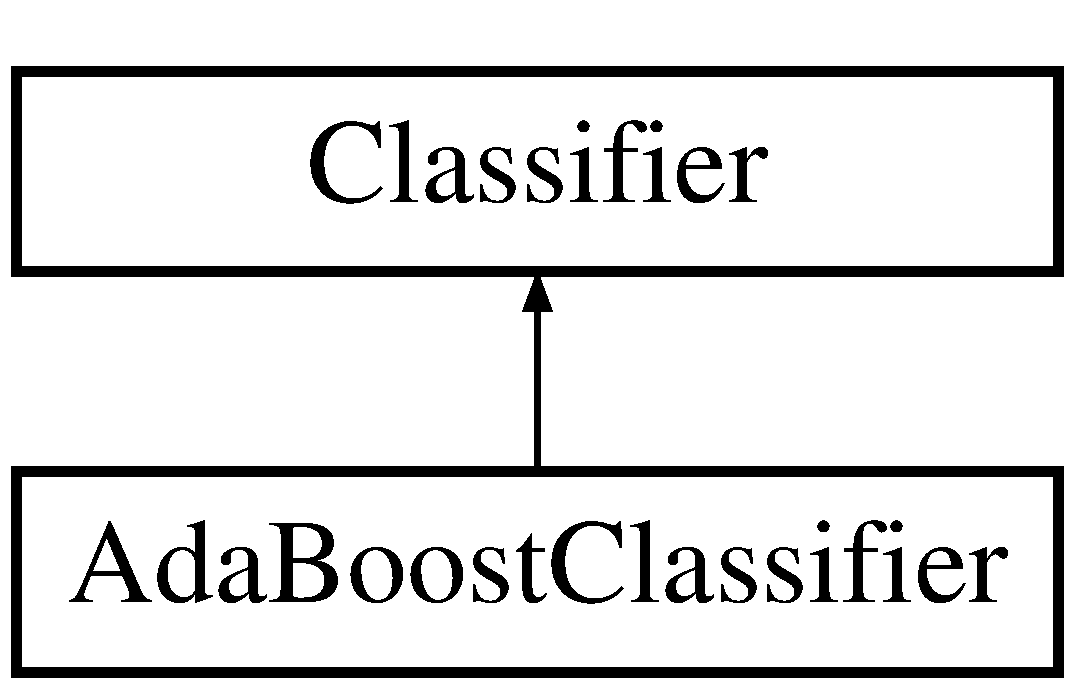
\includegraphics[height=2.000000cm]{classAdaBoostClassifier}
\end{center}
\end{figure}
\subsection*{Public Member Functions}
\begin{DoxyCompactItemize}
\item 
\hypertarget{classAdaBoostClassifier_ab2182542e51a02064f8f5638c5447d07}{}{\bfseries Ada\+Boost\+Classifier} (const char $\ast$filepath)\label{classAdaBoostClassifier_ab2182542e51a02064f8f5638c5447d07}

\item 
\hypertarget{classAdaBoostClassifier_a39f399decacc9920b01b4012b26bdd6c}{}int {\bfseries Classify} (const \hyperlink{classIntegralImage}{Integral\+Image} $\ast$int\+Image, const \hyperlink{classRect}{Rect} \&roi, float scale)\label{classAdaBoostClassifier_a39f399decacc9920b01b4012b26bdd6c}

\end{DoxyCompactItemize}


\subsection{Detailed Description}
\hyperlink{classAdaBoostClassifier}{Ada\+Boost\+Classifier} class. Use many weak classifier to build a strong classifier. \begin{DoxyAuthor}{Author}
Zhengrong Wang. 
\end{DoxyAuthor}


The documentation for this class was generated from the following files\+:\begin{DoxyCompactItemize}
\item 
include/Ada\+Boost\+Classifier.\+h\item 
src/Ada\+Boost\+Classifier.\+cpp\end{DoxyCompactItemize}

\hypertarget{classBKGCutDetector}{}\section{B\+K\+G\+Cut\+Detector Class Reference}
\label{classBKGCutDetector}\index{B\+K\+G\+Cut\+Detector@{B\+K\+G\+Cut\+Detector}}
Inheritance diagram for B\+K\+G\+Cut\+Detector\+:\begin{figure}[H]
\begin{center}
\leavevmode
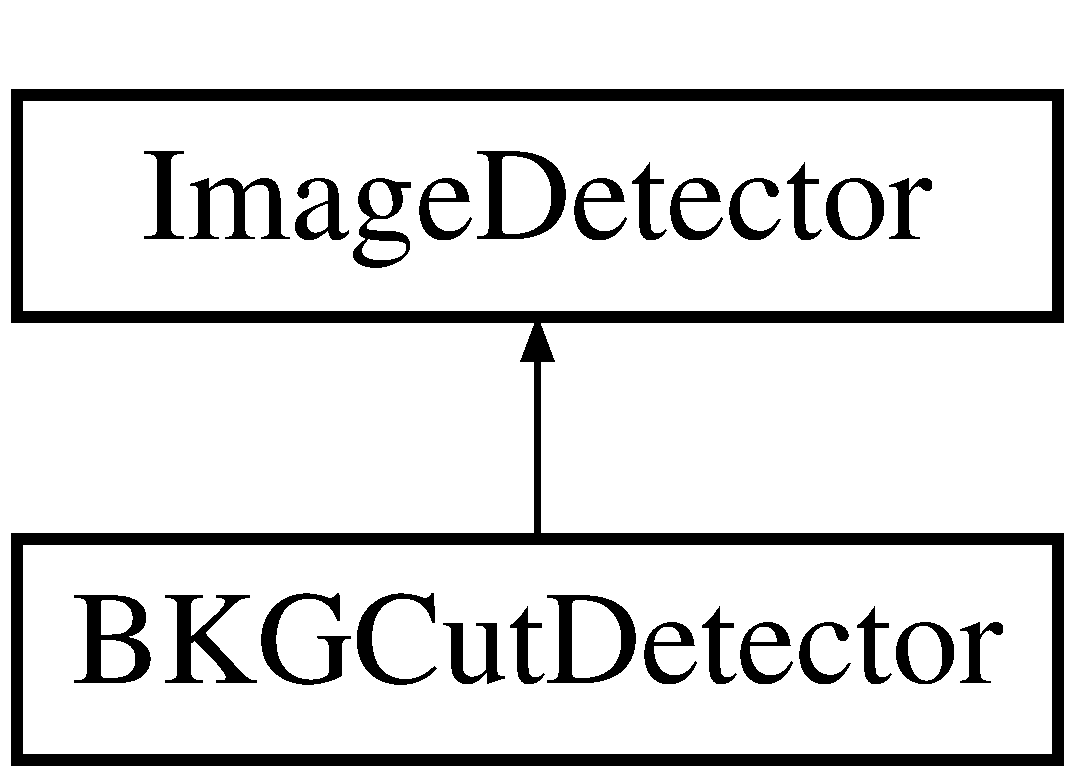
\includegraphics[height=2.000000cm]{classBKGCutDetector}
\end{center}
\end{figure}
\subsection*{Public Member Functions}
\begin{DoxyCompactItemize}
\item 
\hypertarget{classBKGCutDetector_ae2e7fe9cbafab49107aa9e28f05f4822}{}{\bfseries B\+K\+G\+Cut\+Detector} (\hyperlink{classIntegralImage}{Integral\+Image} $\ast$i, \hyperlink{classClassifier}{Classifier} $\ast$c, \hyperlink{structOptions}{Options} \&op)\label{classBKGCutDetector_ae2e7fe9cbafab49107aa9e28f05f4822}

\item 
bool \hyperlink{classBKGCutDetector_ab1e2f37a3436e58197f1429085677b8f}{Detect} (const cv\+::\+Mat \&img, const cv\+::\+Point \&origin, bool is\+Merge=true, const cv\+::\+Mat \&bkg=default\+Background)
\end{DoxyCompactItemize}
\subsection*{Protected Member Functions}
\begin{DoxyCompactItemize}
\item 
\hyperlink{structrect}{rect} \hyperlink{classBKGCutDetector_a2d0179ff253ad09c1549c8437e07736f}{Create\+R\+O\+I} (int x, int y, int roi\+\_\+h, int roi\+\_\+w, int edge\+\_\+width, int height, int width)
\end{DoxyCompactItemize}
\subsection*{Protected Attributes}
\begin{DoxyCompactItemize}
\item 
\hypertarget{classBKGCutDetector_ad1f1988badcfe3f8b6341e0ad7d40e9c}{}feat {\bfseries binary\+Thre}\label{classBKGCutDetector_ad1f1988badcfe3f8b6341e0ad7d40e9c}

\item 
\hypertarget{classBKGCutDetector_a51de970ae40887927077e27092b3d2f4}{}double {\bfseries inv\+Perimeter\+Thre}\label{classBKGCutDetector_a51de970ae40887927077e27092b3d2f4}

\item 
\hypertarget{classBKGCutDetector_a2184787ed50fbe8f30d1a8ef88cb3cc3}{}float {\bfseries min\+Area\+Ratio}\label{classBKGCutDetector_a2184787ed50fbe8f30d1a8ef88cb3cc3}

\item 
\hypertarget{classBKGCutDetector_aea66427f38ba877edf1cac44a242c797}{}float {\bfseries max\+Area\+Ratio}\label{classBKGCutDetector_aea66427f38ba877edf1cac44a242c797}

\end{DoxyCompactItemize}
\subsection*{Additional Inherited Members}


\subsection{Member Function Documentation}
\hypertarget{classBKGCutDetector_a2d0179ff253ad09c1549c8437e07736f}{}\index{B\+K\+G\+Cut\+Detector@{B\+K\+G\+Cut\+Detector}!Create\+R\+O\+I@{Create\+R\+O\+I}}
\index{Create\+R\+O\+I@{Create\+R\+O\+I}!B\+K\+G\+Cut\+Detector@{B\+K\+G\+Cut\+Detector}}
\subsubsection[{Create\+R\+O\+I(int x, int y, int roi\+\_\+h, int roi\+\_\+w, int edge\+\_\+width, int height, int width)}]{\setlength{\rightskip}{0pt plus 5cm}{\bf rect} B\+K\+G\+Cut\+Detector\+::\+Create\+R\+O\+I (
\begin{DoxyParamCaption}
\item[{int}]{x, }
\item[{int}]{y, }
\item[{int}]{roi\+\_\+h, }
\item[{int}]{roi\+\_\+w, }
\item[{int}]{edge\+\_\+width, }
\item[{int}]{height, }
\item[{int}]{width}
\end{DoxyParamCaption}
)\hspace{0.3cm}{\ttfamily [protected]}}\label{classBKGCutDetector_a2d0179ff253ad09c1549c8437e07736f}
Given a rectangle and the size of the original image, expand the rectangle by edge\+\_\+width. 
\begin{DoxyParams}{Parameters}
{\em x} & the x coordinates of the upper-\/left corner. \\
\hline
{\em y} & the y coordinates of the upper-\/left corner. \\
\hline
{\em roi\+\_\+h} & the height of the rectangle. \\
\hline
{\em roi\+\_\+w} & the width of the rectangle. \\
\hline
{\em edge\+\_\+width} & how many pixels you want to expand? \\
\hline
{\em height,width} & the size of the original image. \\
\hline
\end{DoxyParams}
\begin{DoxyReturn}{Returns}
a structure rect. 
\end{DoxyReturn}
\hypertarget{classBKGCutDetector_ab1e2f37a3436e58197f1429085677b8f}{}\index{B\+K\+G\+Cut\+Detector@{B\+K\+G\+Cut\+Detector}!Detect@{Detect}}
\index{Detect@{Detect}!B\+K\+G\+Cut\+Detector@{B\+K\+G\+Cut\+Detector}}
\subsubsection[{Detect(const cv\+::\+Mat \&img, const cv\+::\+Point \&origin, bool is\+Merge=true, const cv\+::\+Mat \&bkg=default\+Background)}]{\setlength{\rightskip}{0pt plus 5cm}bool B\+K\+G\+Cut\+Detector\+::\+Detect (
\begin{DoxyParamCaption}
\item[{const cv\+::\+Mat \&}]{img, }
\item[{const cv\+::\+Point \&}]{origin, }
\item[{bool}]{is\+Merge = {\ttfamily true}, }
\item[{const cv\+::\+Mat \&}]{bkg = {\ttfamily defaultBackground}}
\end{DoxyParamCaption}
)\hspace{0.3cm}{\ttfamily [virtual]}}\label{classBKGCutDetector_ab1e2f37a3436e58197f1429085677b8f}
Detect, return the resutl in a vector. Notice that sometimes we only want to detect in a subregion of the original image, in such case we have to give the origin parameter, which is the coordinates of the upper-\/left corner in the original image. 
\begin{DoxyParams}{Parameters}
{\em img} & the image we need to detect. \\
\hline
{\em origin} & the coordinates of the img\textquotesingle{}s upper-\/left corner in its parents (if any) \\
\hline
{\em bkg} & unused here, for \hyperlink{classBKGCutDetector}{B\+K\+G\+Cut\+Detector}. \\
\hline
{\em is\+Merge} & merge the detection with accumulated evidence. \\
\hline
\end{DoxyParams}
\begin{DoxyReturn}{Returns}
true if everything is fine. 
\end{DoxyReturn}


Reimplemented from \hyperlink{classImageDetector_aca346dbe30c325653c6c9ef1a0ffd0b2}{Image\+Detector}.



The documentation for this class was generated from the following files\+:\begin{DoxyCompactItemize}
\item 
include/B\+K\+G\+Cut\+Detector.\+h\item 
src/B\+K\+G\+Cut\+Detector.\+cpp\end{DoxyCompactItemize}

\hypertarget{classClassifier}{}\section{Classifier Class Reference}
\label{classClassifier}\index{Classifier@{Classifier}}


{\ttfamily \#include $<$Classifier.\+h$>$}

Inheritance diagram for Classifier\+:\begin{figure}[H]
\begin{center}
\leavevmode
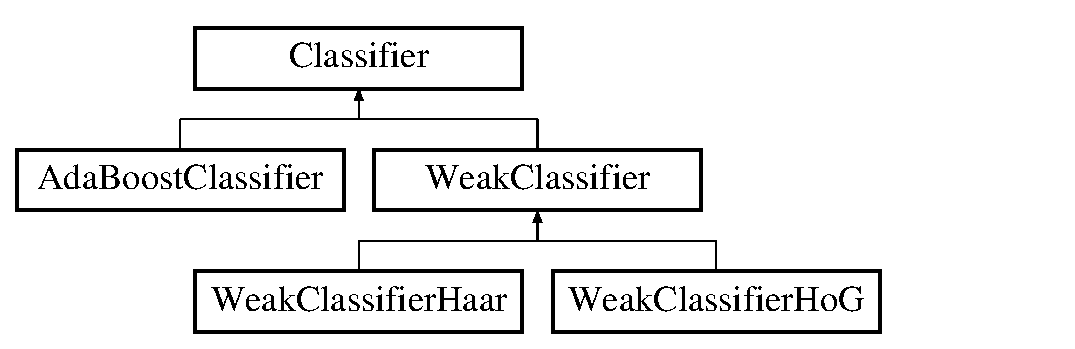
\includegraphics[height=3.000000cm]{classClassifier}
\end{center}
\end{figure}
\subsection*{Public Member Functions}
\begin{DoxyCompactItemize}
\item 
\hypertarget{classClassifier_a126cdbb3bc72d17a6d1184126a7545a0}{}virtual int {\bfseries Classify} (const \hyperlink{classIntegralImage}{Integral\+Image} $\ast$int\+Image, const \hyperlink{classRect}{Rect} \&roi, float scale=1.\+0f)\label{classClassifier_a126cdbb3bc72d17a6d1184126a7545a0}

\item 
\hypertarget{classClassifier_a4e0671ac06531f98373feb917a076c46}{}virtual float {\bfseries Evaluate} (const \hyperlink{classIntegralImage}{Integral\+Image} $\ast$int\+Image, const \hyperlink{classRect}{Rect} \&roi, float scale=1.\+0f)\label{classClassifier_a4e0671ac06531f98373feb917a076c46}

\end{DoxyCompactItemize}


\subsection{Detailed Description}
This is a binary classifier. \begin{DoxyAuthor}{Author}
Zhengrong Wang. 
\end{DoxyAuthor}


The documentation for this class was generated from the following files\+:\begin{DoxyCompactItemize}
\item 
include/Classifier.\+h\item 
src/Classifier.\+cpp\end{DoxyCompactItemize}

\hypertarget{classClassifierSelector}{}\section{Classifier\+Selector Class Reference}
\label{classClassifierSelector}\index{Classifier\+Selector@{Classifier\+Selector}}


{\ttfamily \#include $<$Classifier\+Selector.\+h$>$}

\subsection*{Public Member Functions}
\begin{DoxyCompactItemize}
\item 
\hyperlink{classClassifierSelector_a21eb14f2ad33c62dd94fdfced0d8d9e6}{Classifier\+Selector} (int num\+W, const \hyperlink{classSize}{Size} \&patch\+Size, int num\+B=2)
\item 
\hyperlink{classClassifierSelector_a6bf8094c2c8afde715ab75e729efa4af}{Classifier\+Selector} (int num\+W, \hyperlink{classWeakClassifier}{Weak\+Classifier} $\ast$$\ast$weaks, int num\+B=2)
\item 
void \hyperlink{classClassifierSelector_afd948f69609ddac9d1effb6b899c4d08}{Train} (const \hyperlink{classIntegralImage}{Integral\+Image} $\ast$int\+Image, const \hyperlink{classRect}{Rect} \&roi, int target, float importance, bool $\ast$err\+Mask)
\item 
float \hyperlink{classClassifierSelector_ac7f854deb91854b56f24660b77e702ed}{Get\+Error} (int index=-\/1) const 
\item 
virtual int \hyperlink{classClassifierSelector_aa146f727c4d0d212935885bec3c63ed8}{Select\+Best\+Classifer} (float importance, const bool $\ast$error\+Mask, float $\ast$errors)
\item 
virtual int \hyperlink{classClassifierSelector_ac01dd0dfee31bfbfbbc6b5c28f36a021}{Replace\+Weakest\+Classifier} (float $\ast$errors, const \hyperlink{classSize}{Size} \&patch\+Size)
\item 
virtual void \hyperlink{classClassifierSelector_a07a0717148abf071a4bc3785b72bb3d3}{Replace\+Weakest\+Classifier\+Statistic} (int src, int dst)
\item 
int \hyperlink{classClassifierSelector_acaca168ce5bb47624157c7559cc56108}{Classify} (const \hyperlink{classIntegralImage}{Integral\+Image} $\ast$int\+Image, const \hyperlink{classRect}{Rect} \&roi)
\item 
\hypertarget{classClassifierSelector_a580884e2c9069f9377c1ff49373c22ff}{}float {\bfseries Evaluate} (const \hyperlink{classIntegralImage}{Integral\+Image} $\ast$int\+Image, const \hyperlink{classRect}{Rect} \&roi, int index\+Weak=-\/1)\label{classClassifierSelector_a580884e2c9069f9377c1ff49373c22ff}

\item 
\hypertarget{classClassifierSelector_afd9973943d762de87c049c34bfb8a7fc}{}\hyperlink{classWeakClassifier}{Weak\+Classifier} $\ast$$\ast$ {\bfseries Get\+Classifier\+Pool} () const \label{classClassifierSelector_afd9973943d762de87c049c34bfb8a7fc}

\item 
\hypertarget{classClassifierSelector_a942422f09080814f8e9b914f06a2a403}{}void {\bfseries Set\+Classifier\+Pool} (\hyperlink{classWeakClassifier}{Weak\+Classifier} $\ast$$\ast$weaks)\label{classClassifierSelector_a942422f09080814f8e9b914f06a2a403}

\item 
\hypertarget{classClassifierSelector_a81b945b9d43952b71c5de2c026083f9c}{}int {\bfseries Get\+New\+Backup} ()\label{classClassifierSelector_a81b945b9d43952b71c5de2c026083f9c}

\end{DoxyCompactItemize}


\subsection{Detailed Description}
Select the best classifier from some weak classifiers. Here we only use \hyperlink{classWeakClassifierHaar}{Weak\+Classifier\+Haar}. Used in online boosting classifier. \begin{DoxyAuthor}{Author}
Zhengrong Wang. 
\end{DoxyAuthor}


\subsection{Constructor \& Destructor Documentation}
\hypertarget{classClassifierSelector_a21eb14f2ad33c62dd94fdfced0d8d9e6}{}\index{Classifier\+Selector@{Classifier\+Selector}!Classifier\+Selector@{Classifier\+Selector}}
\index{Classifier\+Selector@{Classifier\+Selector}!Classifier\+Selector@{Classifier\+Selector}}
\subsubsection[{Classifier\+Selector(int num\+W, const Size \&patch\+Size, int num\+B=2)}]{\setlength{\rightskip}{0pt plus 5cm}Classifier\+Selector\+::\+Classifier\+Selector (
\begin{DoxyParamCaption}
\item[{int}]{num\+W, }
\item[{const {\bf Size} \&}]{patch\+Size, }
\item[{int}]{num\+B = {\ttfamily 2}}
\end{DoxyParamCaption}
)}\label{classClassifierSelector_a21eb14f2ad33c62dd94fdfced0d8d9e6}
Build a classifier selector with some Weak\+Classifier\+Haars. 
\begin{DoxyParams}{Parameters}
{\em num\+W} & \# weak classifiers. \\
\hline
{\em patch\+Size} & the patch size used in weak classifiers. \\
\hline
{\em num\+B} & \# weak classifiers for subsititution. \\
\hline
\end{DoxyParams}
\hypertarget{classClassifierSelector_a6bf8094c2c8afde715ab75e729efa4af}{}\index{Classifier\+Selector@{Classifier\+Selector}!Classifier\+Selector@{Classifier\+Selector}}
\index{Classifier\+Selector@{Classifier\+Selector}!Classifier\+Selector@{Classifier\+Selector}}
\subsubsection[{Classifier\+Selector(int num\+W, Weak\+Classifier $\ast$$\ast$weaks, int num\+B=2)}]{\setlength{\rightskip}{0pt plus 5cm}Classifier\+Selector\+::\+Classifier\+Selector (
\begin{DoxyParamCaption}
\item[{int}]{num\+W, }
\item[{{\bf Weak\+Classifier} $\ast$$\ast$}]{weaks, }
\item[{int}]{num\+B = {\ttfamily 2}}
\end{DoxyParamCaption}
)}\label{classClassifierSelector_a6bf8094c2c8afde715ab75e729efa4af}
Build a classifier selector from some outside weakclassifier array. 
\begin{DoxyParams}{Parameters}
{\em weaks} & the array of weak classifiers. \\
\hline
\end{DoxyParams}


\subsection{Member Function Documentation}
\hypertarget{classClassifierSelector_acaca168ce5bb47624157c7559cc56108}{}\index{Classifier\+Selector@{Classifier\+Selector}!Classify@{Classify}}
\index{Classify@{Classify}!Classifier\+Selector@{Classifier\+Selector}}
\subsubsection[{Classify(const Integral\+Image $\ast$int\+Image, const Rect \&roi)}]{\setlength{\rightskip}{0pt plus 5cm}int Classifier\+Selector\+::\+Classify (
\begin{DoxyParamCaption}
\item[{const {\bf Integral\+Image} $\ast$}]{int\+Image, }
\item[{const {\bf Rect} \&}]{roi}
\end{DoxyParamCaption}
)}\label{classClassifierSelector_acaca168ce5bb47624157c7559cc56108}
Evaluate a feature. \begin{DoxyReturn}{Returns}
1 for pos, -\/1 for neg. 
\end{DoxyReturn}
\hypertarget{classClassifierSelector_ac7f854deb91854b56f24660b77e702ed}{}\index{Classifier\+Selector@{Classifier\+Selector}!Get\+Error@{Get\+Error}}
\index{Get\+Error@{Get\+Error}!Classifier\+Selector@{Classifier\+Selector}}
\subsubsection[{Get\+Error(int index=-\/1) const }]{\setlength{\rightskip}{0pt plus 5cm}float Classifier\+Selector\+::\+Get\+Error (
\begin{DoxyParamCaption}
\item[{int}]{index = {\ttfamily -\/1}}
\end{DoxyParamCaption}
) const}\label{classClassifierSelector_ac7f854deb91854b56f24660b77e702ed}
\begin{DoxyReturn}{Returns}
the error rate of this seletor, or any specific classifier. 
\end{DoxyReturn}
\hypertarget{classClassifierSelector_ac01dd0dfee31bfbfbbc6b5c28f36a021}{}\index{Classifier\+Selector@{Classifier\+Selector}!Replace\+Weakest\+Classifier@{Replace\+Weakest\+Classifier}}
\index{Replace\+Weakest\+Classifier@{Replace\+Weakest\+Classifier}!Classifier\+Selector@{Classifier\+Selector}}
\subsubsection[{Replace\+Weakest\+Classifier(float $\ast$errors, const Size \&patch\+Size)}]{\setlength{\rightskip}{0pt plus 5cm}int Classifier\+Selector\+::\+Replace\+Weakest\+Classifier (
\begin{DoxyParamCaption}
\item[{float $\ast$}]{errors, }
\item[{const {\bf Size} \&}]{patch\+Size}
\end{DoxyParamCaption}
)\hspace{0.3cm}{\ttfamily [virtual]}}\label{classClassifierSelector_ac01dd0dfee31bfbfbbc6b5c28f36a021}
Replace the weakest classifier. 
\begin{DoxyParams}{Parameters}
{\em errors} & a buffer contains the error rate. \\
\hline
\end{DoxyParams}
\begin{DoxyReturn}{Returns}
\+: the index of the replaced classifier. 
\end{DoxyReturn}
\hypertarget{classClassifierSelector_a07a0717148abf071a4bc3785b72bb3d3}{}\index{Classifier\+Selector@{Classifier\+Selector}!Replace\+Weakest\+Classifier\+Statistic@{Replace\+Weakest\+Classifier\+Statistic}}
\index{Replace\+Weakest\+Classifier\+Statistic@{Replace\+Weakest\+Classifier\+Statistic}!Classifier\+Selector@{Classifier\+Selector}}
\subsubsection[{Replace\+Weakest\+Classifier\+Statistic(int src, int dst)}]{\setlength{\rightskip}{0pt plus 5cm}void Classifier\+Selector\+::\+Replace\+Weakest\+Classifier\+Statistic (
\begin{DoxyParamCaption}
\item[{int}]{src, }
\item[{int}]{dst}
\end{DoxyParamCaption}
)\hspace{0.3cm}{\ttfamily [virtual]}}\label{classClassifierSelector_a07a0717148abf071a4bc3785b72bb3d3}
Only replace the weight. Used when the weak classifier is from outside. \hypertarget{classClassifierSelector_aa146f727c4d0d212935885bec3c63ed8}{}\index{Classifier\+Selector@{Classifier\+Selector}!Select\+Best\+Classifer@{Select\+Best\+Classifer}}
\index{Select\+Best\+Classifer@{Select\+Best\+Classifer}!Classifier\+Selector@{Classifier\+Selector}}
\subsubsection[{Select\+Best\+Classifer(float importance, const bool $\ast$error\+Mask, float $\ast$errors)}]{\setlength{\rightskip}{0pt plus 5cm}int Classifier\+Selector\+::\+Select\+Best\+Classifer (
\begin{DoxyParamCaption}
\item[{float}]{importance, }
\item[{const bool $\ast$}]{error\+Mask, }
\item[{float $\ast$}]{errors}
\end{DoxyParamCaption}
)\hspace{0.3cm}{\ttfamily [virtual]}}\label{classClassifierSelector_aa146f727c4d0d212935885bec3c63ed8}
Select the best classifier. 
\begin{DoxyParams}{Parameters}
{\em in} & importance\+: the weight of this sample. \\
\hline
{\em in} & error\+Mask\+: true if the classifer makes mistake on this sample. \\
\hline
{\em out} & errors\+: a buffer contains the error rates of each classifier. \\
\hline
\end{DoxyParams}
\begin{DoxyReturn}{Returns}
index of new selected classifier. 
\end{DoxyReturn}
\hypertarget{classClassifierSelector_afd948f69609ddac9d1effb6b899c4d08}{}\index{Classifier\+Selector@{Classifier\+Selector}!Train@{Train}}
\index{Train@{Train}!Classifier\+Selector@{Classifier\+Selector}}
\subsubsection[{Train(const Integral\+Image $\ast$int\+Image, const Rect \&roi, int target, float importance, bool $\ast$err\+Mask)}]{\setlength{\rightskip}{0pt plus 5cm}void Classifier\+Selector\+::\+Train (
\begin{DoxyParamCaption}
\item[{const {\bf Integral\+Image} $\ast$}]{int\+Image, }
\item[{const {\bf Rect} \&}]{roi, }
\item[{int}]{target, }
\item[{float}]{importance, }
\item[{bool $\ast$}]{err\+Mask}
\end{DoxyParamCaption}
)}\label{classClassifierSelector_afd948f69609ddac9d1effb6b899c4d08}
Train the weak classifiers. 
\begin{DoxyParams}{Parameters}
{\em int\+Image} & the integral image. \\
\hline
{\em roi} & the region of the target. \\
\hline
{\em target} & 1 for pos, -\/1 for neg. \\
\hline
{\em importance} & the weight of this sample. \\
\hline
{\em out} & err\+Mask\+: update the error mask array. \\
\hline
\end{DoxyParams}


The documentation for this class was generated from the following files\+:\begin{DoxyCompactItemize}
\item 
include/Classifier\+Selector.\+h\item 
src/Classifier\+Selector.\+cpp\end{DoxyCompactItemize}

\hypertarget{classClassifierThreshold}{}\section{Classifier\+Threshold$<$ N $>$ Class Template Reference}
\label{classClassifierThreshold}\index{Classifier\+Threshold$<$ N $>$@{Classifier\+Threshold$<$ N $>$}}


{\ttfamily \#include $<$Classifier\+Threshold.\+h$>$}

\subsection*{Public Member Functions}
\begin{DoxyCompactItemize}
\item 
void \hyperlink{classClassifierThreshold_ae9bae753884c08a274b2204af8e97340}{Update} (const \hyperlink{classFeature}{Feature} \&feature, int target)
\item 
int \hyperlink{classClassifierThreshold_a74dff1a82e6d201d6bceedd198e1f105}{Classify} (const \hyperlink{classFeature}{Feature} \&feature)
\item 
\hypertarget{classClassifierThreshold_a1f566cc491d863b15828561cbdfcd7a0}{}void {\bfseries Reset} ()\label{classClassifierThreshold_a1f566cc491d863b15828561cbdfcd7a0}

\item 
\hypertarget{classClassifierThreshold_ac5ea1576c2b8f51dc2643c7f6dbe7724}{}void $\ast$ {\bfseries Get\+Distribution} (int target) const \label{classClassifierThreshold_ac5ea1576c2b8f51dc2643c7f6dbe7724}

\end{DoxyCompactItemize}


\subsection{Detailed Description}
\subsubsection*{template$<$int N$>$class Classifier\+Threshold$<$ N $>$}

This class use N-\/\+D Gaussian distribution for pos and neg data set. Given a feature, it returns whether it\textquotesingle{}s positive or negative. \begin{DoxyAuthor}{Author}
Zhengrong Wang. 
\end{DoxyAuthor}


\subsection{Member Function Documentation}
\hypertarget{classClassifierThreshold_a74dff1a82e6d201d6bceedd198e1f105}{}\index{Classifier\+Threshold@{Classifier\+Threshold}!Classify@{Classify}}
\index{Classify@{Classify}!Classifier\+Threshold@{Classifier\+Threshold}}
\subsubsection[{Classify(const Feature \&feature)}]{\setlength{\rightskip}{0pt plus 5cm}template$<$int N$>$ int {\bf Classifier\+Threshold}$<$ N $>$\+::Classify (
\begin{DoxyParamCaption}
\item[{const {\bf Feature} \&}]{feature}
\end{DoxyParamCaption}
)}\label{classClassifierThreshold_a74dff1a82e6d201d6bceedd198e1f105}
Evaluate the feature. Use the simple Euclidean distance to pos and neg cluster. 
\begin{DoxyParams}{Parameters}
{\em feature} & the feature extracted, should be N dimension. \\
\hline
\end{DoxyParams}
\begin{DoxyReturn}{Returns}
int\+: 1 for positive, -\/1 for negative. 
\end{DoxyReturn}
\hypertarget{classClassifierThreshold_ae9bae753884c08a274b2204af8e97340}{}\index{Classifier\+Threshold@{Classifier\+Threshold}!Update@{Update}}
\index{Update@{Update}!Classifier\+Threshold@{Classifier\+Threshold}}
\subsubsection[{Update(const Feature \&feature, int target)}]{\setlength{\rightskip}{0pt plus 5cm}template$<$int N$>$ void {\bf Classifier\+Threshold}$<$ N $>$\+::Update (
\begin{DoxyParamCaption}
\item[{const {\bf Feature} \&}]{feature, }
\item[{int}]{target}
\end{DoxyParamCaption}
)}\label{classClassifierThreshold_ae9bae753884c08a274b2204af8e97340}
Use Kalman filter to update the pos and neg cluster. 
\begin{DoxyParams}{Parameters}
{\em feature} & the feature extracted, should be N dimension. \\
\hline
{\em target} & positive $>$ 0, negative $<$= 0. \\
\hline
\end{DoxyParams}


The documentation for this class was generated from the following file\+:\begin{DoxyCompactItemize}
\item 
include/Classifier\+Threshold.\+h\end{DoxyCompactItemize}

\hypertarget{classConnectedComponents}{}\section{Connected\+Components Class Reference}
\label{classConnectedComponents}\index{Connected\+Components@{Connected\+Components}}
\subsection*{Static Public Member Functions}
\begin{DoxyCompactItemize}
\item 
\hypertarget{classConnectedComponents_ad59d9b6bc16ad0b2c37552c5b236aade}{}static void {\bfseries Find} (cv\+::\+Mat \&binary, bool poly\+Approx, float inv\+Perim\+Scale)\label{classConnectedComponents_ad59d9b6bc16ad0b2c37552c5b236aade}

\end{DoxyCompactItemize}
\subsection*{Static Public Attributes}
\begin{DoxyCompactItemize}
\item 
\hypertarget{classConnectedComponents_ae8f2cf051af196924705311ab181d661}{}static std\+::vector$<$ std\+::vector$<$ cv\+::\+Point $>$ $>$ {\bfseries contours}\label{classConnectedComponents_ae8f2cf051af196924705311ab181d661}

\item 
static const cv\+::\+Mat {\bfseries element}
\end{DoxyCompactItemize}


\subsection{Member Data Documentation}
\hypertarget{classConnectedComponents_a7620c576b46a91864d30a6b2ab56eedb}{}\index{Connected\+Components@{Connected\+Components}!element@{element}}
\index{element@{element}!Connected\+Components@{Connected\+Components}}
\subsubsection[{element}]{\setlength{\rightskip}{0pt plus 5cm}const cv\+::\+Mat Connected\+Components\+::element\hspace{0.3cm}{\ttfamily [static]}}\label{classConnectedComponents_a7620c576b46a91864d30a6b2ab56eedb}
{\bfseries Initial value\+:}
\begin{DoxyCode}
= cv::getStructuringElement(
    MPRPH\_ELEM, 
    cv::Size(2 * MORPH\_SIZE + 1, 2 * MORPH\_SIZE + 1), 
    cv::Point(MORPH\_SIZE, MORPH\_SIZE))
\end{DoxyCode}


The documentation for this class was generated from the following files\+:\begin{DoxyCompactItemize}
\item 
include/Connected\+Components.\+h\item 
src/Connected\+Components.\+cpp\end{DoxyCompactItemize}

\hypertarget{classEstimatedGaussianDistribution}{}\section{Estimated\+Gaussian\+Distribution$<$ N $>$ Class Template Reference}
\label{classEstimatedGaussianDistribution}\index{Estimated\+Gaussian\+Distribution$<$ N $>$@{Estimated\+Gaussian\+Distribution$<$ N $>$}}


{\ttfamily \#include $<$Estimated\+Gaussian\+Distribution.\+h$>$}

\subsection*{Public Member Functions}
\begin{DoxyCompactItemize}
\item 
\hypertarget{classEstimatedGaussianDistribution_afe5b507d908e2669fe8ea708a87e7c3b}{}{\bfseries Estimated\+Gaussian\+Distribution} (float pm=1000.\+0f, float ps=1000.\+0f, float rm=0.\+01f, float rs=0.\+01f)\label{classEstimatedGaussianDistribution_afe5b507d908e2669fe8ea708a87e7c3b}

\item 
void \hyperlink{classEstimatedGaussianDistribution_a2be4f792f6916c45825801980f648e9a}{Reset} (float pm=1000.\+0f, float ps=1000.\+0f, float rm=0.\+01f, float rs=0.\+01f)
\item 
void \hyperlink{classEstimatedGaussianDistribution_a340e3a01f89d62ddab06a0dbc8e9fe3c}{Update} (const float $\ast$value)
\item 
\hypertarget{classEstimatedGaussianDistribution_a7d2ccd30d2252f59c37a810a986e78a0}{}void {\bfseries Set\+Values} (const float $\ast$m, const float $\ast$s)\label{classEstimatedGaussianDistribution_a7d2ccd30d2252f59c37a810a986e78a0}

\end{DoxyCompactItemize}
\subsection*{Public Attributes}
\begin{DoxyCompactItemize}
\item 
\hypertarget{classEstimatedGaussianDistribution_a0ce3513e3ecbe1882a3a1d6aa4aeb10f}{}float {\bfseries mean} \mbox{[}N\mbox{]}\label{classEstimatedGaussianDistribution_a0ce3513e3ecbe1882a3a1d6aa4aeb10f}

\item 
\hypertarget{classEstimatedGaussianDistribution_af8e85818690b3d1dc18ef467cb5fcc01}{}float {\bfseries sigma} \mbox{[}N\mbox{]}\label{classEstimatedGaussianDistribution_af8e85818690b3d1dc18ef467cb5fcc01}

\item 
\hypertarget{classEstimatedGaussianDistribution_a5240d7947f5f386125209bf9b4a04712}{}float {\bfseries p\+Mean}\label{classEstimatedGaussianDistribution_a5240d7947f5f386125209bf9b4a04712}

\item 
\hypertarget{classEstimatedGaussianDistribution_a5f59468f2b623f2072977cdfc91c86a5}{}float {\bfseries p\+Sigma}\label{classEstimatedGaussianDistribution_a5f59468f2b623f2072977cdfc91c86a5}

\item 
\hypertarget{classEstimatedGaussianDistribution_ae2cdb30a07eced903acd22fd8cf93ca5}{}float {\bfseries r\+Mean}\label{classEstimatedGaussianDistribution_ae2cdb30a07eced903acd22fd8cf93ca5}

\item 
\hypertarget{classEstimatedGaussianDistribution_af8400eefcec90df5ce67f95c9c3f25fd}{}float {\bfseries r\+Sigma}\label{classEstimatedGaussianDistribution_af8400eefcec90df5ce67f95c9c3f25fd}

\end{DoxyCompactItemize}


\subsection{Detailed Description}
\subsubsection*{template$<$int N$>$class Estimated\+Gaussian\+Distribution$<$ N $>$}

Estimate a N dimension Gaussian distribution with Kalman filter. 

\subsection{Member Function Documentation}
\hypertarget{classEstimatedGaussianDistribution_a2be4f792f6916c45825801980f648e9a}{}\index{Estimated\+Gaussian\+Distribution@{Estimated\+Gaussian\+Distribution}!Reset@{Reset}}
\index{Reset@{Reset}!Estimated\+Gaussian\+Distribution@{Estimated\+Gaussian\+Distribution}}
\subsubsection[{Reset(float pm=1000.\+0f, float ps=1000.\+0f, float rm=0.\+01f, float rs=0.\+01f)}]{\setlength{\rightskip}{0pt plus 5cm}template$<$int N$>$ void {\bf Estimated\+Gaussian\+Distribution}$<$ N $>$\+::Reset (
\begin{DoxyParamCaption}
\item[{float}]{pm = {\ttfamily 1000.0f}, }
\item[{float}]{ps = {\ttfamily 1000.0f}, }
\item[{float}]{rm = {\ttfamily 0.01f}, }
\item[{float}]{rs = {\ttfamily 0.01f}}
\end{DoxyParamCaption}
)\hspace{0.3cm}{\ttfamily [inline]}}\label{classEstimatedGaussianDistribution_a2be4f792f6916c45825801980f648e9a}
Reset everything to the start state. \hypertarget{classEstimatedGaussianDistribution_a340e3a01f89d62ddab06a0dbc8e9fe3c}{}\index{Estimated\+Gaussian\+Distribution@{Estimated\+Gaussian\+Distribution}!Update@{Update}}
\index{Update@{Update}!Estimated\+Gaussian\+Distribution@{Estimated\+Gaussian\+Distribution}}
\subsubsection[{Update(const float $\ast$value)}]{\setlength{\rightskip}{0pt plus 5cm}template$<$int N$>$ void {\bf Estimated\+Gaussian\+Distribution}$<$ N $>$\+::Update (
\begin{DoxyParamCaption}
\item[{const float $\ast$}]{value}
\end{DoxyParamCaption}
)}\label{classEstimatedGaussianDistribution_a340e3a01f89d62ddab06a0dbc8e9fe3c}
Use Kalman filter to update the Gaussian distribution. 

The documentation for this class was generated from the following file\+:\begin{DoxyCompactItemize}
\item 
include/Estimated\+Gaussian\+Distribution.\+h\end{DoxyCompactItemize}

\hypertarget{classFeature}{}\section{Feature Class Reference}
\label{classFeature}\index{Feature@{Feature}}


{\ttfamily \#include $<$Feature.\+h$>$}

\subsection*{Public Member Functions}
\begin{DoxyCompactItemize}
\item 
\hypertarget{classFeature_a2b74be536afddf041660d4e7cf380a79}{}{\bfseries Feature} (int size=0)\label{classFeature_a2b74be536afddf041660d4e7cf380a79}

\item 
\hypertarget{classFeature_a91798da6497d0b3a2837d78daf246476}{}void {\bfseries Resize} (int new\+Size)\label{classFeature_a91798da6497d0b3a2837d78daf246476}

\end{DoxyCompactItemize}
\subsection*{Public Attributes}
\begin{DoxyCompactItemize}
\item 
\hypertarget{classFeature_ae90dde1871e9e81ce6b7b5f99080e4f3}{}feat $\ast$ {\bfseries data}\label{classFeature_ae90dde1871e9e81ce6b7b5f99080e4f3}

\item 
\hypertarget{classFeature_af4d2343cf558bf32746a777a2c272fac}{}int {\bfseries capacity}\label{classFeature_af4d2343cf558bf32746a777a2c272fac}

\end{DoxyCompactItemize}


\subsection{Detailed Description}
Basically it\textquotesingle{}s just a vector. \begin{DoxyAuthor}{Author}
Zhengrong Wang 
\end{DoxyAuthor}


The documentation for this class was generated from the following files\+:\begin{DoxyCompactItemize}
\item 
include/Feature.\+h\item 
src/Feature.\+cpp\end{DoxyCompactItemize}

\hypertarget{classFeatureExtractor}{}\section{Feature\+Extractor Class Reference}
\label{classFeatureExtractor}\index{Feature\+Extractor@{Feature\+Extractor}}
Inheritance diagram for Feature\+Extractor\+:\begin{figure}[H]
\begin{center}
\leavevmode
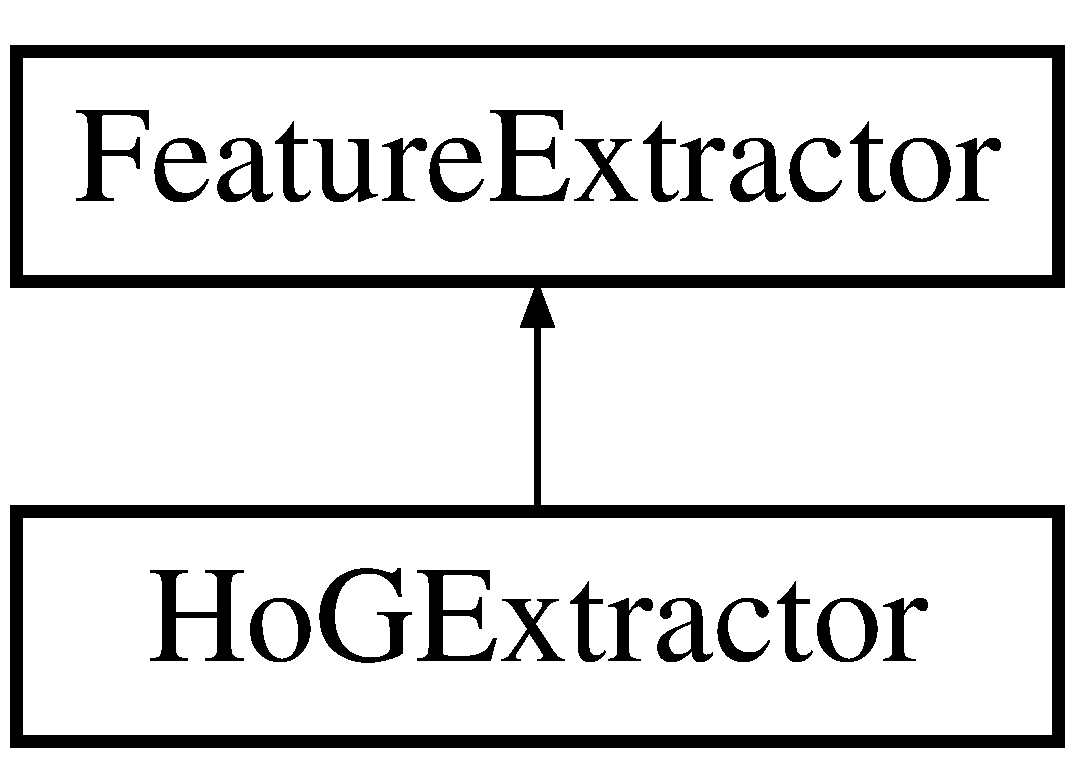
\includegraphics[height=2.000000cm]{classFeatureExtractor}
\end{center}
\end{figure}
\subsection*{Public Member Functions}
\begin{DoxyCompactItemize}
\item 
\hypertarget{classFeatureExtractor_a2dd7d3294e8c93f8e0faa68c2233adcc}{}virtual void {\bfseries Extract} (int width, int height, int i, int j, \hyperlink{classFeature}{Feature} $\ast$feature)=0\label{classFeatureExtractor_a2dd7d3294e8c93f8e0faa68c2233adcc}

\item 
\hypertarget{classFeatureExtractor_aabb0751deb4be6180130e7c0d8d644fd}{}virtual void {\bfseries Preprocess} (const cv\+::\+Mat \&img)\label{classFeatureExtractor_aabb0751deb4be6180130e7c0d8d644fd}

\end{DoxyCompactItemize}


The documentation for this class was generated from the following file\+:\begin{DoxyCompactItemize}
\item 
include/Feature\+Extractor.\+h\end{DoxyCompactItemize}

\hypertarget{classGrayScaleIntegralImage}{}\section{Gray\+Scale\+Integral\+Image Class Reference}
\label{classGrayScaleIntegralImage}\index{Gray\+Scale\+Integral\+Image@{Gray\+Scale\+Integral\+Image}}


{\ttfamily \#include $<$Gray\+Scale\+Integral\+Image.\+h$>$}

Inheritance diagram for Gray\+Scale\+Integral\+Image\+:\begin{figure}[H]
\begin{center}
\leavevmode
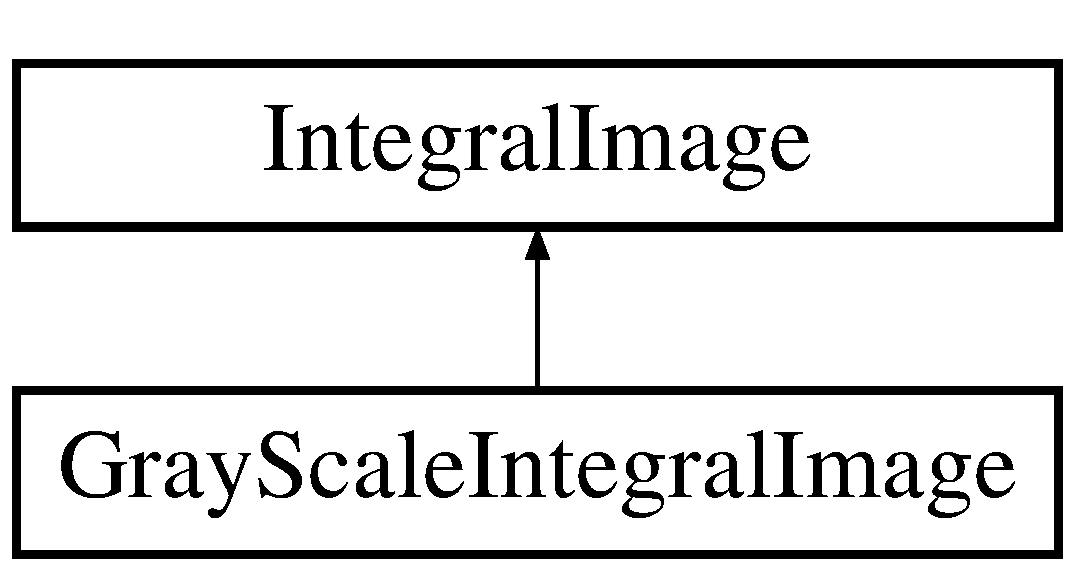
\includegraphics[height=2.000000cm]{classGrayScaleIntegralImage}
\end{center}
\end{figure}
\subsection*{Public Member Functions}
\begin{DoxyCompactItemize}
\item 
\hypertarget{classGrayScaleIntegralImage_a1b15921690e2b519fe0bc0310d303a9b}{}{\bfseries Gray\+Scale\+Integral\+Image} (const cv\+::\+Mat \&img)\label{classGrayScaleIntegralImage_a1b15921690e2b519fe0bc0310d303a9b}

\item 
\hypertarget{classGrayScaleIntegralImage_a8ca08cb9b71f23f2ca331db8ab35f144}{}{\bfseries Gray\+Scale\+Integral\+Image} (int w, int h)\label{classGrayScaleIntegralImage_a8ca08cb9b71f23f2ca331db8ab35f144}

\item 
\hypertarget{classGrayScaleIntegralImage_a234716e692aad7557fc4debc94a9780f}{}void {\bfseries Calculate\+Int} (const cv\+::\+Mat \&img)\label{classGrayScaleIntegralImage_a234716e692aad7557fc4debc94a9780f}

\item 
\hypertarget{classGrayScaleIntegralImage_aecfdc4fa33aa5a15e340eef5b5456681}{}unsigned int {\bfseries Get\+Sum} (const \hyperlink{classRect}{Rect} \&roi) const \label{classGrayScaleIntegralImage_aecfdc4fa33aa5a15e340eef5b5456681}

\end{DoxyCompactItemize}
\subsection*{Additional Inherited Members}


\subsection{Detailed Description}
The basic integral image. Integral the grayscale intensity. This can be used in Haar like feature. \begin{DoxyAuthor}{Author}
Zhengrong Wang. 
\end{DoxyAuthor}


The documentation for this class was generated from the following files\+:\begin{DoxyCompactItemize}
\item 
include/Gray\+Scale\+Integral\+Image.\+h\item 
src/Gray\+Scale\+Integral\+Image.\+cpp\end{DoxyCompactItemize}

\hypertarget{classHaarFeature}{}\section{Haar\+Feature Class Reference}
\label{classHaarFeature}\index{Haar\+Feature@{Haar\+Feature}}


{\ttfamily \#include $<$Haar\+Feature.\+h$>$}

\subsection*{Public Member Functions}
\begin{DoxyCompactItemize}
\item 
\hypertarget{classHaarFeature_a54b1a86c01341793d393cce0e8ff7d72}{}{\bfseries Haar\+Feature} (const \hyperlink{classSize}{Size} \&patch\+Size)\label{classHaarFeature_a54b1a86c01341793d393cce0e8ff7d72}

\item 
\hypertarget{classHaarFeature_a293df81066b1cba52baac9904e155b20}{}void {\bfseries Get\+Initial\+Distribution} (\hyperlink{classEstimatedGaussianDistribution}{Estimated\+Gaussian\+Distribution}$<$ 1 $>$ $\ast$distribution) const \label{classHaarFeature_a293df81066b1cba52baac9904e155b20}

\item 
\hypertarget{classHaarFeature_a9b74485ba82429c7311a0aa490a2f1b6}{}bool {\bfseries Extract} (const \hyperlink{classIntegralImage}{Integral\+Image} $\ast$int\+Image, const \hyperlink{classRect}{Rect} \&roi, \hyperlink{classFeature}{Feature} $\ast$feature)\label{classHaarFeature_a9b74485ba82429c7311a0aa490a2f1b6}

\item 
\hypertarget{classHaarFeature_a40d755bcccf0ea1e5ebb154eea7d26ac}{}float {\bfseries Get\+Response} ()\label{classHaarFeature_a40d755bcccf0ea1e5ebb154eea7d26ac}

\item 
\hypertarget{classHaarFeature_aa2abfada29f6848fef8d45c4c85479c1}{}int {\bfseries Get\+Num\+Areas} ()\label{classHaarFeature_aa2abfada29f6848fef8d45c4c85479c1}

\item 
\hypertarget{classHaarFeature_a25936c7b13e76190a58ae737de1de360}{}int $\ast$ {\bfseries Get\+Weights} ()\label{classHaarFeature_a25936c7b13e76190a58ae737de1de360}

\end{DoxyCompactItemize}


\subsection{Detailed Description}
Haar \hyperlink{classFeature}{Feature} class. Extract a Haar like feature from the image. \begin{DoxyAuthor}{Author}
Zhengrong Wang 
\end{DoxyAuthor}


The documentation for this class was generated from the following files\+:\begin{DoxyCompactItemize}
\item 
include/Haar\+Feature.\+h\item 
src/Haar\+Feature.\+cpp\end{DoxyCompactItemize}

\hypertarget{classHoGExtractor}{}\section{Ho\+G\+Extractor Class Reference}
\label{classHoGExtractor}\index{Ho\+G\+Extractor@{Ho\+G\+Extractor}}
Inheritance diagram for Ho\+G\+Extractor\+:\begin{figure}[H]
\begin{center}
\leavevmode
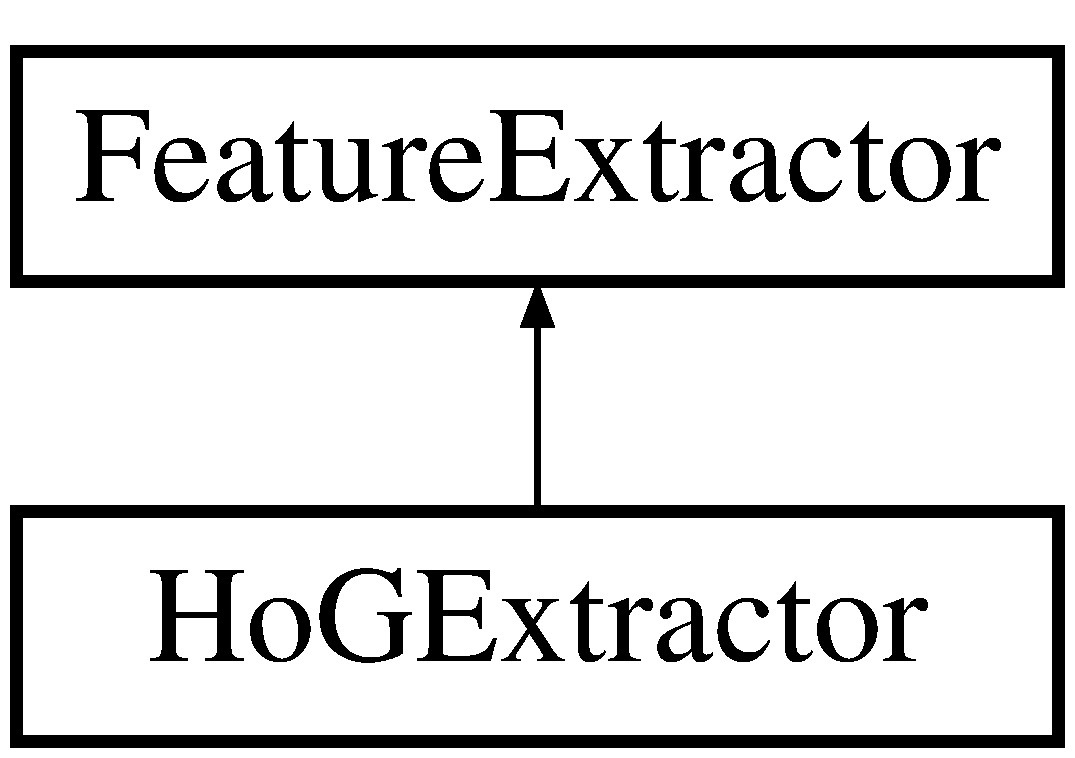
\includegraphics[height=2.000000cm]{classHoGExtractor}
\end{center}
\end{figure}
\subsection*{Public Member Functions}
\begin{DoxyCompactItemize}
\item 
\hypertarget{classHoGExtractor_acc0ace70caba09e835940c3abdb4965f}{}{\bfseries Ho\+G\+Extractor} (int width, int height)\label{classHoGExtractor_acc0ace70caba09e835940c3abdb4965f}

\item 
\hypertarget{classHoGExtractor_acad10e438c39ed5d9f8e812d3f6f3c80}{}void {\bfseries Preprocess} (const cv\+::\+Mat \&img)\label{classHoGExtractor_acad10e438c39ed5d9f8e812d3f6f3c80}

\item 
\hypertarget{classHoGExtractor_a0fe8f6fe37ff5e18cf27cee49a67dbc4}{}void {\bfseries Extract} (int width, int height, int i, int j, \hyperlink{classFeature}{Feature} $\ast$feature)\label{classHoGExtractor_a0fe8f6fe37ff5e18cf27cee49a67dbc4}

\end{DoxyCompactItemize}


The documentation for this class was generated from the following files\+:\begin{DoxyCompactItemize}
\item 
include/Feature\+Extractor.\+h\item 
src/Feature\+Extractor.\+cpp\end{DoxyCompactItemize}

\hypertarget{classHoGFeature}{}\section{Ho\+G\+Feature Class Reference}
\label{classHoGFeature}\index{Ho\+G\+Feature@{Ho\+G\+Feature}}


{\ttfamily \#include $<$Ho\+G\+Feature.\+h$>$}

\subsection*{Public Member Functions}
\begin{DoxyCompactItemize}
\item 
\hypertarget{classHoGFeature_a1e8f745b4991e6f97c1ce16ba981baa1}{}{\bfseries Ho\+G\+Feature} (int offset\+W, int offset\+H, int w, int h)\label{classHoGFeature_a1e8f745b4991e6f97c1ce16ba981baa1}

\item 
bool \hyperlink{classHoGFeature_aae463c642f7ff64980eebe9f0519eae0}{Extract} (const \hyperlink{classIntegralImage}{Integral\+Image} $\ast$int\+Image, const \hyperlink{classRect}{Rect} \&roi, \hyperlink{classFeature}{Feature} $\ast$feature, float scale=1.\+0f) const 
\end{DoxyCompactItemize}


\subsection{Detailed Description}
Extract the Ho\+G of subregion in the roi. \begin{DoxyAuthor}{Author}
Zhengrong Wang. 
\end{DoxyAuthor}


\subsection{Member Function Documentation}
\hypertarget{classHoGFeature_aae463c642f7ff64980eebe9f0519eae0}{}\index{Ho\+G\+Feature@{Ho\+G\+Feature}!Extract@{Extract}}
\index{Extract@{Extract}!Ho\+G\+Feature@{Ho\+G\+Feature}}
\subsubsection[{Extract(const Integral\+Image $\ast$int\+Image, const Rect \&roi, Feature $\ast$feature, float scale=1.\+0f) const }]{\setlength{\rightskip}{0pt plus 5cm}bool Ho\+G\+Feature\+::\+Extract (
\begin{DoxyParamCaption}
\item[{const {\bf Integral\+Image} $\ast$}]{int\+Image, }
\item[{const {\bf Rect} \&}]{roi, }
\item[{{\bf Feature} $\ast$}]{feature, }
\item[{float}]{scale = {\ttfamily 1.0f}}
\end{DoxyParamCaption}
) const}\label{classHoGFeature_aae463c642f7ff64980eebe9f0519eae0}
The patch is like this\+:

$<$-\/-\/-\/---\mbox{[}scaled\+With / 2\mbox{]}-\/-\/-\/---$^\wedge$-\/-\/-\/-\/---\mbox{[}scaled\+Width -\/ scaled\+Width / 2\mbox{]}-\/-\/-\/---$>$ $\vert$ $\vert$ $\vert$ \mbox{[}scaled\+Height / 2\mbox{]} $\vert$ $\vert$ $\vert$ $\vert$ $\vert$ $^\wedge$-\/-\/-\/-\/-\/-\/-\/-\/-\/-\/-\/-\/-\/-\/-\/-\/-\/-\/-\/-\/-\/-\/-\/-\/-\/---$^\wedge$-\/-\/-\/-\/-\/-\/-\/-\/-\/-\/-\/-\/-\/-\/-\/-\/-\/-\/-\/-\/-\/-\/-\/-\/-\/-\/-\/-\/-\/-\/-\/-\/-\/-\/-\/-\/-\/-\/-\/-\/-\/---$^\wedge$ $\vert$ $\vert$ $\vert$ \mbox{[}scaled\+Height -\/ $\vert$ $\vert$ scaled\+Height / 2\mbox{]} $\vert$ $\vert$ $\vert$ $\vert$ $\vert$ $^\wedge$-\/-\/-\/-\/-\/-\/-\/-\/-\/-\/-\/-\/-\/-\/-\/-\/-\/-\/-\/-\/-\/-\/-\/-\/-\/---$^\wedge$-\/-\/-\/-\/-\/-\/-\/-\/-\/-\/-\/-\/-\/-\/-\/-\/-\/-\/-\/-\/-\/-\/-\/-\/-\/-\/-\/-\/-\/-\/-\/-\/-\/-\/-\/-\/-\/-\/-\/-\/-\/---$^\wedge$

The documentation for this class was generated from the following files\+:\begin{DoxyCompactItemize}
\item 
include/Ho\+G\+Feature.\+h\item 
src/Ho\+G\+Feature.\+cpp\end{DoxyCompactItemize}

\hypertarget{classHoGIntegralImage}{}\section{Ho\+G\+Integral\+Image Class Reference}
\label{classHoGIntegralImage}\index{Ho\+G\+Integral\+Image@{Ho\+G\+Integral\+Image}}
Inheritance diagram for Ho\+G\+Integral\+Image\+:\begin{figure}[H]
\begin{center}
\leavevmode
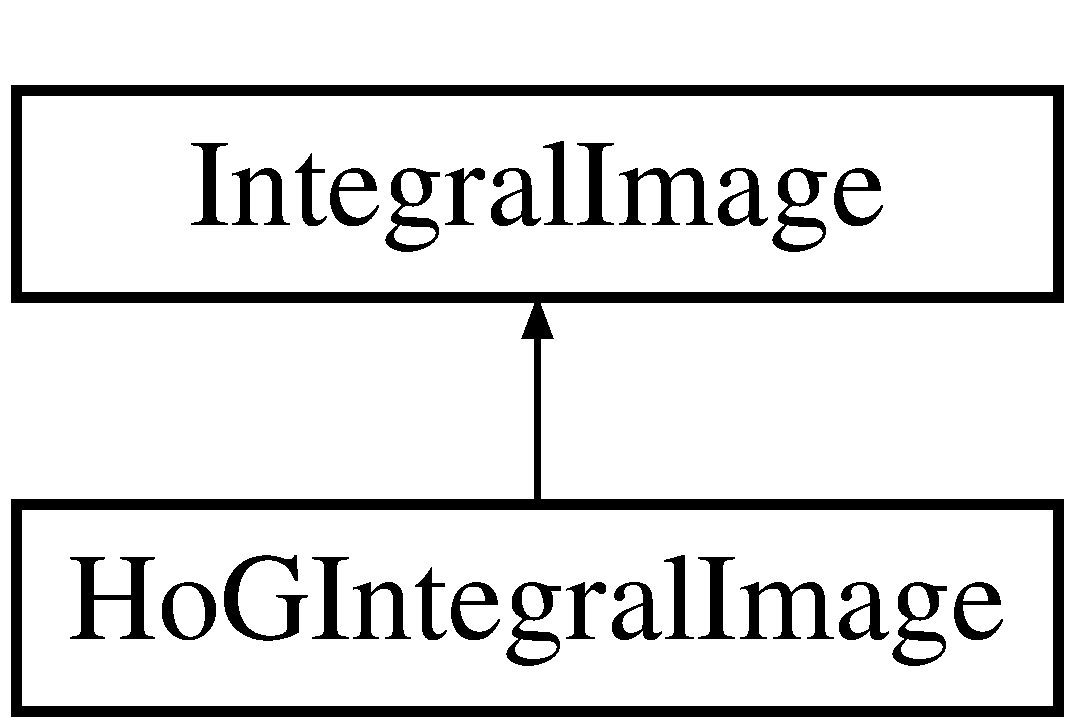
\includegraphics[height=2.000000cm]{classHoGIntegralImage}
\end{center}
\end{figure}
\subsection*{Public Member Functions}
\begin{DoxyCompactItemize}
\item 
\hypertarget{classHoGIntegralImage_a3005a86adb82824baa52194dc7263e04}{}{\bfseries Ho\+G\+Integral\+Image} (const cv\+::\+Mat \&img)\label{classHoGIntegralImage_a3005a86adb82824baa52194dc7263e04}

\item 
\hypertarget{classHoGIntegralImage_a8f177c758e21a588d4f872f7f7ebcb44}{}{\bfseries Ho\+G\+Integral\+Image} (int w, int h)\label{classHoGIntegralImage_a8f177c758e21a588d4f872f7f7ebcb44}

\item 
\hypertarget{classHoGIntegralImage_aede37af7488a0b63b9516dab670fdee5}{}void {\bfseries Calculate\+Int} (const cv\+::\+Mat \&img)\label{classHoGIntegralImage_aede37af7488a0b63b9516dab670fdee5}

\item 
\hypertarget{classHoGIntegralImage_a57eef64a949491e3cb9a3e37d4710e11}{}void {\bfseries Get\+Sum} (const \hyperlink{classRect}{Rect} \&roi, float $\ast$result) const \label{classHoGIntegralImage_a57eef64a949491e3cb9a3e37d4710e11}

\end{DoxyCompactItemize}
\subsection*{Additional Inherited Members}


The documentation for this class was generated from the following files\+:\begin{DoxyCompactItemize}
\item 
include/Ho\+G\+Integral\+Image.\+h\item 
src/Ho\+G\+Integral\+Image.\+cpp\end{DoxyCompactItemize}

\hypertarget{classImageDetector}{}\section{Image\+Detector Class Reference}
\label{classImageDetector}\index{Image\+Detector@{Image\+Detector}}
Inheritance diagram for Image\+Detector\+:\begin{figure}[H]
\begin{center}
\leavevmode
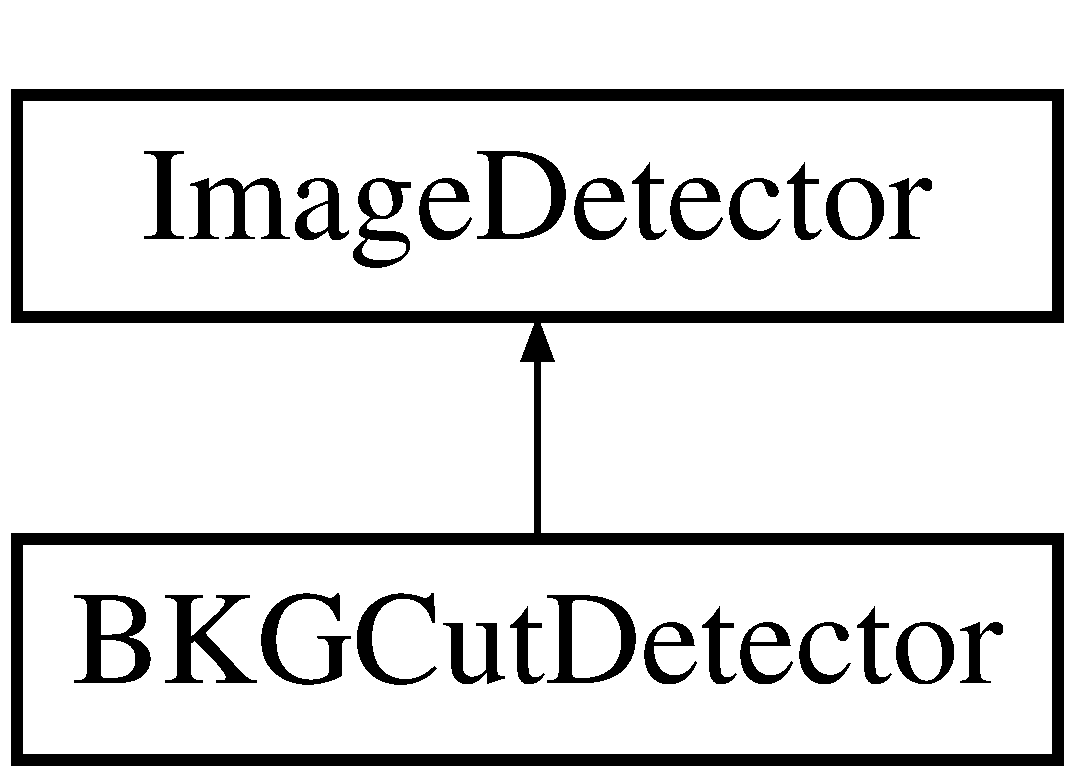
\includegraphics[height=2.000000cm]{classImageDetector}
\end{center}
\end{figure}
\subsection*{Public Member Functions}
\begin{DoxyCompactItemize}
\item 
\hypertarget{classImageDetector_ae661e19aa8fce824ff3e159efae1dd71}{}{\bfseries Image\+Detector} (\hyperlink{classIntegralImage}{Integral\+Image} $\ast$i, \hyperlink{classClassifier}{Classifier} $\ast$c, \hyperlink{structOptions}{Options} \&op)\label{classImageDetector_ae661e19aa8fce824ff3e159efae1dd71}

\item 
virtual bool \hyperlink{classImageDetector_aca346dbe30c325653c6c9ef1a0ffd0b2}{Detect} (const cv\+::\+Mat \&img, const cv\+::\+Point \&origin=cv\+::\+Point(0, 0), bool is\+Merge=true, const cv\+::\+Mat \&bkg=default\+Background)
\item 
\hypertarget{classImageDetector_a866cc9f2e6b109ea8a897e96c4b106a1}{}void {\bfseries Draw\+Detection} (cv\+::\+Mat \&img)\label{classImageDetector_a866cc9f2e6b109ea8a897e96c4b106a1}

\item 
\hypertarget{classImageDetector_a2293f8558975b3404dae1ed077d47580}{}void {\bfseries Clear} ()\label{classImageDetector_a2293f8558975b3404dae1ed077d47580}

\end{DoxyCompactItemize}
\subsection*{Public Attributes}
\begin{DoxyCompactItemize}
\item 
\hypertarget{classImageDetector_a38b4eb45a8506399546219cc17886f7c}{}\hyperlink{classPool}{Pool}$<$ \hyperlink{structrect}{rect} $>$ {\bfseries dets}\label{classImageDetector_a38b4eb45a8506399546219cc17886f7c}

\end{DoxyCompactItemize}
\subsection*{Protected Member Functions}
\begin{DoxyCompactItemize}
\item 
\hypertarget{classImageDetector_ab8ae540f23e94c8acdb0cc0893bffe6d}{}bool {\bfseries Is\+Equal} (const \hyperlink{structrect}{rect} \&r1, const \hyperlink{structrect}{rect} \&r2) const \label{classImageDetector_ab8ae540f23e94c8acdb0cc0893bffe6d}

\item 
\hypertarget{classImageDetector_a52d903953d90efcde6e727910254f77d}{}bool {\bfseries Is\+Overlap} (const \hyperlink{structrect}{rect} \&r, const \hyperlink{structrect}{rect} \&t) const \label{classImageDetector_a52d903953d90efcde6e727910254f77d}

\end{DoxyCompactItemize}
\subsection*{Protected Attributes}
\begin{DoxyCompactItemize}
\item 
\hypertarget{classImageDetector_a604ac20e008c67fe067fc01bfcf16c2b}{}\hyperlink{classIntegralImage}{Integral\+Image} $\ast$ {\bfseries int\+Image}\label{classImageDetector_a604ac20e008c67fe067fc01bfcf16c2b}

\item 
\hypertarget{classImageDetector_a85a290b68f969c9fab97926b38e256a1}{}\hyperlink{classClassifier}{Classifier} $\ast$ {\bfseries classifier}\label{classImageDetector_a85a290b68f969c9fab97926b38e256a1}

\item 
\hypertarget{classImageDetector_a34ef14c4268fdd84bff58c8484a489e3}{}feat {\bfseries scale\+Min}\label{classImageDetector_a34ef14c4268fdd84bff58c8484a489e3}

\item 
\hypertarget{classImageDetector_ad5a391221072002a5700e37114acf430}{}feat {\bfseries scale\+Max}\label{classImageDetector_ad5a391221072002a5700e37114acf430}

\item 
\hypertarget{classImageDetector_a865fd99867e339649be938525d09a30b}{}feat {\bfseries scale\+Step}\label{classImageDetector_a865fd99867e339649be938525d09a30b}

\item 
\hypertarget{classImageDetector_a0e67a6d3973d15482ce58f10550c2645}{}int {\bfseries slide\+Step}\label{classImageDetector_a0e67a6d3973d15482ce58f10550c2645}

\item 
\hypertarget{classImageDetector_a5b18257894ec3cc6ff90488a15db70cd}{}int {\bfseries evidence}\label{classImageDetector_a5b18257894ec3cc6ff90488a15db70cd}

\item 
\hypertarget{classImageDetector_a912db87e0677e3315e433b6603abaeab}{}int {\bfseries model\+Height}\label{classImageDetector_a912db87e0677e3315e433b6603abaeab}

\item 
\hypertarget{classImageDetector_ac20bd858ca20dbfec53c7c2d66bdbf39}{}int {\bfseries model\+Width}\label{classImageDetector_ac20bd858ca20dbfec53c7c2d66bdbf39}

\item 
\hypertarget{classImageDetector_a75b3168312f048818022f8c4973dfcdb}{}\hyperlink{classPool}{Pool}$<$ \hyperlink{structrect}{rect} $>$ {\bfseries temp}\label{classImageDetector_a75b3168312f048818022f8c4973dfcdb}

\end{DoxyCompactItemize}


\subsection{Member Function Documentation}
\hypertarget{classImageDetector_aca346dbe30c325653c6c9ef1a0ffd0b2}{}\index{Image\+Detector@{Image\+Detector}!Detect@{Detect}}
\index{Detect@{Detect}!Image\+Detector@{Image\+Detector}}
\subsubsection[{Detect(const cv\+::\+Mat \&img, const cv\+::\+Point \&origin=cv\+::\+Point(0, 0), bool is\+Merge=true, const cv\+::\+Mat \&bkg=default\+Background)}]{\setlength{\rightskip}{0pt plus 5cm}bool Image\+Detector\+::\+Detect (
\begin{DoxyParamCaption}
\item[{const cv\+::\+Mat \&}]{img, }
\item[{const cv\+::\+Point \&}]{origin = {\ttfamily cv\+:\+:Point(0,~0)}, }
\item[{bool}]{is\+Merge = {\ttfamily true}, }
\item[{const cv\+::\+Mat \&}]{bkg = {\ttfamily defaultBackground}}
\end{DoxyParamCaption}
)\hspace{0.3cm}{\ttfamily [virtual]}}\label{classImageDetector_aca346dbe30c325653c6c9ef1a0ffd0b2}
Detect, return the resutl in a vector. Notice that sometimes we only want to detect in a subregion of the original image, in such case we have to give the origin parameter, which is the coordinates of the upper-\/left corner in the original image. 
\begin{DoxyParams}{Parameters}
{\em img} & the image we need to detect. \\
\hline
{\em origin} & the coordinates of the img\textquotesingle{}s upper-\/left corner in its parents (if any) \\
\hline
{\em bkg} & unused here, for \hyperlink{classBKGCutDetector}{B\+K\+G\+Cut\+Detector}. \\
\hline
{\em is\+Merge} & merge the detection with accumulated evidence. \\
\hline
\end{DoxyParams}
\begin{DoxyReturn}{Returns}
true if everything is fine. 
\end{DoxyReturn}


Reimplemented in \hyperlink{classBKGCutDetector_ab1e2f37a3436e58197f1429085677b8f}{B\+K\+G\+Cut\+Detector}.



The documentation for this class was generated from the following files\+:\begin{DoxyCompactItemize}
\item 
include/Image\+Detector.\+h\item 
src/Image\+Detector.\+cpp\end{DoxyCompactItemize}

\hypertarget{classIntegralImage}{}\section{Integral\+Image Class Reference}
\label{classIntegralImage}\index{Integral\+Image@{Integral\+Image}}


{\ttfamily \#include $<$Integral\+Image.\+h$>$}

Inheritance diagram for Integral\+Image\+:\begin{figure}[H]
\begin{center}
\leavevmode
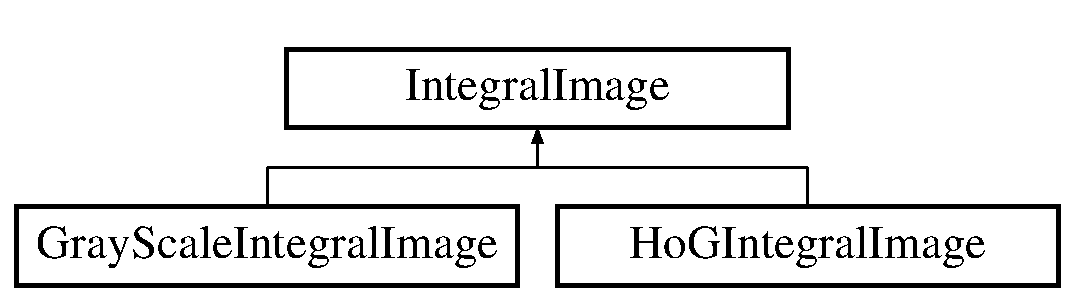
\includegraphics[height=2.000000cm]{classIntegralImage}
\end{center}
\end{figure}
\subsection*{Public Member Functions}
\begin{DoxyCompactItemize}
\item 
\hypertarget{classIntegralImage_a3cfe7e68c1e757de16b10c6a8d04bb0d}{}{\bfseries Integral\+Image} (const cv\+::\+Mat \&img)\label{classIntegralImage_a3cfe7e68c1e757de16b10c6a8d04bb0d}

\item 
\hypertarget{classIntegralImage_aee12d9b9aefddb1ea18c4bd0fa6dcbcc}{}{\bfseries Integral\+Image} (int w, int h)\label{classIntegralImage_aee12d9b9aefddb1ea18c4bd0fa6dcbcc}

\item 
\hypertarget{classIntegralImage_ae578410b9fca079c2274cfe1b0e45a12}{}virtual void {\bfseries Calculate\+Int} (const cv\+::\+Mat \&img)=0\label{classIntegralImage_ae578410b9fca079c2274cfe1b0e45a12}

\item 
\hypertarget{classIntegralImage_a8e9c76dadb4a74863991f3ca32c4e33d}{}virtual unsigned int {\bfseries Get\+Sum} (const \hyperlink{classRect}{Rect} \&roi) const \label{classIntegralImage_a8e9c76dadb4a74863991f3ca32c4e33d}

\item 
\hypertarget{classIntegralImage_a339adc6f566e0c66dd2e0fca979e5308}{}virtual void {\bfseries Get\+Sum} (const \hyperlink{classRect}{Rect} \&roi, float $\ast$result) const \label{classIntegralImage_a339adc6f566e0c66dd2e0fca979e5308}

\end{DoxyCompactItemize}
\subsection*{Public Attributes}
\begin{DoxyCompactItemize}
\item 
\hypertarget{classIntegralImage_a0e48dfba6ab1a43b7df5944272fa125a}{}int {\bfseries width}\label{classIntegralImage_a0e48dfba6ab1a43b7df5944272fa125a}

\item 
\hypertarget{classIntegralImage_aa3a261ce530a860004fb057881f83782}{}int {\bfseries height}\label{classIntegralImage_aa3a261ce530a860004fb057881f83782}

\end{DoxyCompactItemize}


\subsection{Detailed Description}
\begin{DoxyAuthor}{Author}
Zhengrong Wang 
\end{DoxyAuthor}


The documentation for this class was generated from the following files\+:\begin{DoxyCompactItemize}
\item 
include/Integral\+Image.\+h\item 
src/Integral\+Image.\+cpp\end{DoxyCompactItemize}

\hypertarget{classMultiTracker}{}\section{Multi\+Tracker Class Reference}
\label{classMultiTracker}\index{Multi\+Tracker@{Multi\+Tracker}}
Inheritance diagram for Multi\+Tracker\+:\begin{figure}[H]
\begin{center}
\leavevmode
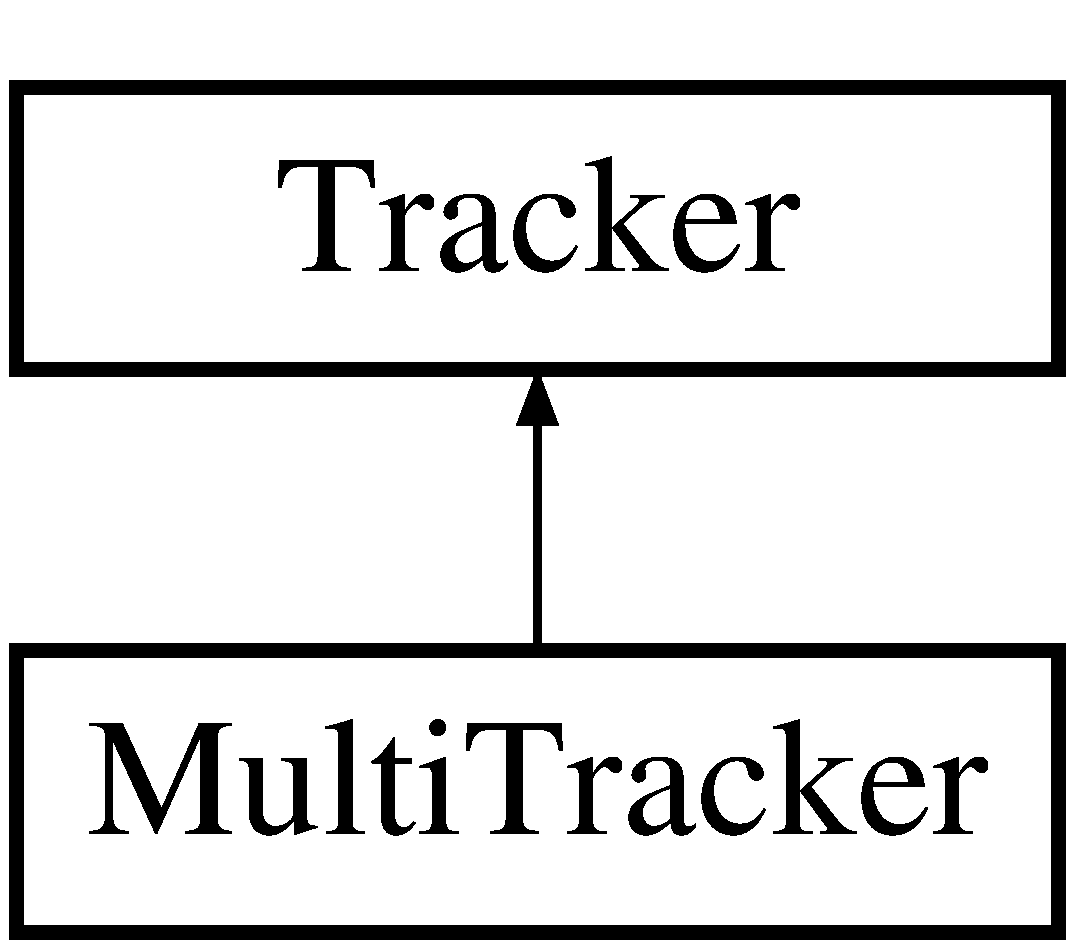
\includegraphics[height=2.000000cm]{classMultiTracker}
\end{center}
\end{figure}
\subsection*{Public Member Functions}
\begin{DoxyCompactItemize}
\item 
\hyperlink{classMultiTracker_a313f4618102c4d62b0e67244cef65e93}{Multi\+Tracker} (\hyperlink{classImageDetector}{Image\+Detector} $\ast$detector, const \hyperlink{classSize}{Size} \&img\+Size, const \hyperlink{structOptions}{Options} \&opts)
\item 
\hypertarget{classMultiTracker_a20c07da355cd6c7deded2303960aef56}{}void {\bfseries Track} (cv\+::\+Video\+Capture \&in, cv\+::\+Video\+Writer \&out, const cv\+::\+Mat \&bkg=default\+Background)\label{classMultiTracker_a20c07da355cd6c7deded2303960aef56}

\end{DoxyCompactItemize}


\subsection{Constructor \& Destructor Documentation}
\hypertarget{classMultiTracker_a313f4618102c4d62b0e67244cef65e93}{}\index{Multi\+Tracker@{Multi\+Tracker}!Multi\+Tracker@{Multi\+Tracker}}
\index{Multi\+Tracker@{Multi\+Tracker}!Multi\+Tracker@{Multi\+Tracker}}
\subsubsection[{Multi\+Tracker(\+Image\+Detector $\ast$detector, const Size \&img\+Size, const Options \&opts)}]{\setlength{\rightskip}{0pt plus 5cm}Multi\+Tracker\+::\+Multi\+Tracker (
\begin{DoxyParamCaption}
\item[{{\bf Image\+Detector} $\ast$}]{detector, }
\item[{const {\bf Size} \&}]{img\+Size, }
\item[{const {\bf Options} \&}]{opts}
\end{DoxyParamCaption}
)}\label{classMultiTracker_a313f4618102c4d62b0e67244cef65e93}

\begin{DoxyParams}{Parameters}
{\em detector} & image detector \\
\hline
{\em size} & size of a frame  opts all the options \\
\hline
\end{DoxyParams}


The documentation for this class was generated from the following files\+:\begin{DoxyCompactItemize}
\item 
include/Multi\+Tracker.\+h\item 
src/Multi\+Tracker.\+cpp\end{DoxyCompactItemize}

\hypertarget{structOptions}{}\section{Options Struct Reference}
\label{structOptions}\index{Options@{Options}}


{\ttfamily \#include $<$Options.\+h$>$}

\subsection*{Public Attributes}
\begin{DoxyCompactItemize}
\item 
\hypertarget{structOptions_affdfe3fdb610773968554bc1a80176dd}{}feat {\bfseries scale\+Min}\label{structOptions_affdfe3fdb610773968554bc1a80176dd}

\item 
\hypertarget{structOptions_a0652a70e49763e95db9f61f2f70f7bf7}{}feat {\bfseries scale\+Max}\label{structOptions_a0652a70e49763e95db9f61f2f70f7bf7}

\item 
\hypertarget{structOptions_adb2992a2cc6928303de986d7a1052a00}{}feat {\bfseries scale\+Step}\label{structOptions_adb2992a2cc6928303de986d7a1052a00}

\item 
\hypertarget{structOptions_aa7e47c7146ac77408d3ab3a8028185fd}{}feat {\bfseries binary\+Thre}\label{structOptions_aa7e47c7146ac77408d3ab3a8028185fd}

\item 
\hypertarget{structOptions_a802f1830b28814d67ba43b69e2549910}{}int {\bfseries slide\+Step}\label{structOptions_a802f1830b28814d67ba43b69e2549910}

\item 
\hypertarget{structOptions_a96a28ee7a8e6655bce8cdf47f0d3f64a}{}int {\bfseries evidence}\label{structOptions_a96a28ee7a8e6655bce8cdf47f0d3f64a}

\item 
\hypertarget{structOptions_a28c5d1648f5bf5c9e9461a59262a6e13}{}int {\bfseries model\+Height}\label{structOptions_a28c5d1648f5bf5c9e9461a59262a6e13}

\item 
\hypertarget{structOptions_a06b085d0c70d1e423b85b7e9db5fd9fc}{}int {\bfseries model\+Width}\label{structOptions_a06b085d0c70d1e423b85b7e9db5fd9fc}

\item 
\hypertarget{structOptions_ae412ce0aa974ad8ce47b65d1ec581317}{}float {\bfseries inv\+Perimeter\+Ratio}\label{structOptions_ae412ce0aa974ad8ce47b65d1ec581317}

\item 
\hypertarget{structOptions_a93bd7acdd3ffe585fe0cd7d8db629bb0}{}float {\bfseries min\+Area\+Ratio}\label{structOptions_a93bd7acdd3ffe585fe0cd7d8db629bb0}

\item 
\hypertarget{structOptions_ac0f2ee6436490e03ea9ddd105b4329a3}{}float {\bfseries max\+Area\+Ratio}\label{structOptions_ac0f2ee6436490e03ea9ddd105b4329a3}

\item 
\hypertarget{structOptions_adbea7c640a0dde1cf38a3471d287c881}{}int {\bfseries n\+Particles}\label{structOptions_adbea7c640a0dde1cf38a3471d287c881}

\item 
\hypertarget{structOptions_a18576350a93e3981b992338c1d93be12}{}\hyperlink{classRect}{Rect} {\bfseries target}\label{structOptions_a18576350a93e3981b992338c1d93be12}

\item 
\hypertarget{structOptions_a53812ab25a97fb1ec3680287ec52c86a}{}\hyperlink{classPoint2D}{Point2\+D} {\bfseries init\+Velocity}\label{structOptions_a53812ab25a97fb1ec3680287ec52c86a}

\item 
\hypertarget{structOptions_a23805896bf1b571da4cdbd14839e085e}{}int {\bfseries num\+Selectors}\label{structOptions_a23805896bf1b571da4cdbd14839e085e}

\item 
\hypertarget{structOptions_a12b717b1c67077ac9253ec39c5ff5b90}{}int {\bfseries num\+Weak\+Classifiers}\label{structOptions_a12b717b1c67077ac9253ec39c5ff5b90}

\item 
\hypertarget{structOptions_ac07db4461bb07073094cacc1ded099bb}{}int {\bfseries num\+Backups}\label{structOptions_ac07db4461bb07073094cacc1ded099bb}

\item 
\hypertarget{structOptions_abc31130c59c69ce3391ef2fcfade8dda}{}float {\bfseries dist\+Weight}\label{structOptions_abc31130c59c69ce3391ef2fcfade8dda}

\item 
\hypertarget{structOptions_a14ed11d9f166d5a51686b3d7a374d321}{}float {\bfseries velocity\+Thre}\label{structOptions_a14ed11d9f166d5a51686b3d7a374d321}

\item 
\hypertarget{structOptions_a992480e3ae3d5d552a6db7468176ad29}{}float {\bfseries velocity\+Sigma\+Const}\label{structOptions_a992480e3ae3d5d552a6db7468176ad29}

\item 
\hypertarget{structOptions_abf189d7ae3c26b01ee4cd45c8ff725fa}{}float {\bfseries match\+Thre}\label{structOptions_abf189d7ae3c26b01ee4cd45c8ff725fa}

\item 
\hypertarget{structOptions_a289959230f28e7dd539dabd153c140c2}{}int {\bfseries targets\+Free\+List\+Capacity}\label{structOptions_a289959230f28e7dd539dabd153c140c2}

\item 
\hypertarget{structOptions_a87453b1a266c31e2ab74a4e25b8cf7cc}{}float {\bfseries detection\+Weight}\label{structOptions_a87453b1a266c31e2ab74a4e25b8cf7cc}

\end{DoxyCompactItemize}


\subsection{Detailed Description}
All the options here.

\begin{DoxyAuthor}{Author}
Zhengrong Wang 
\end{DoxyAuthor}


The documentation for this struct was generated from the following file\+:\begin{DoxyCompactItemize}
\item 
include/Options.\+h\end{DoxyCompactItemize}

\hypertarget{classParticleFilter}{}\section{Particle\+Filter Class Reference}
\label{classParticleFilter}\index{Particle\+Filter@{Particle\+Filter}}


{\ttfamily \#include $<$Particle\+Filter.\+h$>$}

Inheritance diagram for Particle\+Filter\+:\begin{figure}[H]
\begin{center}
\leavevmode
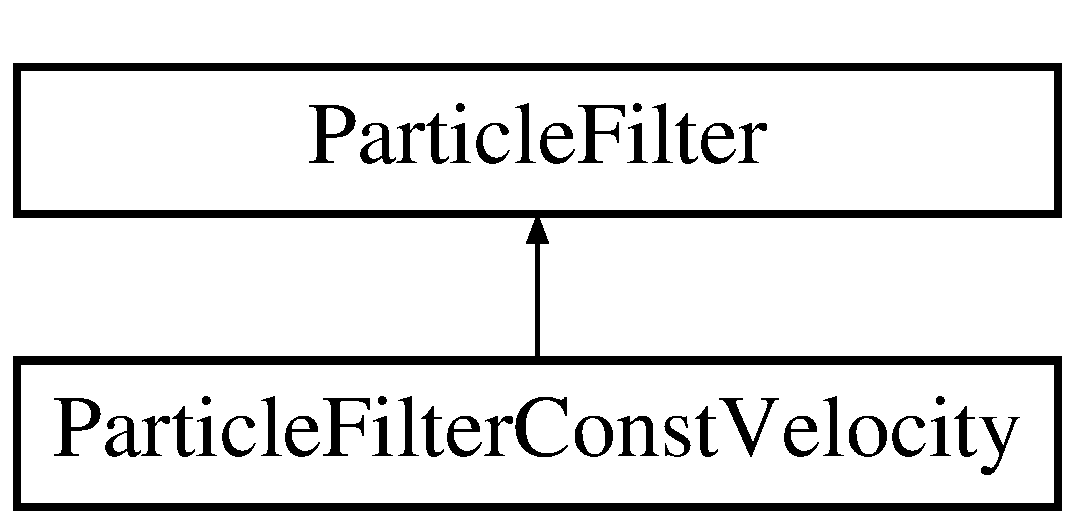
\includegraphics[height=2.000000cm]{classParticleFilter}
\end{center}
\end{figure}
\subsection*{Public Member Functions}
\begin{DoxyCompactItemize}
\item 
\hyperlink{classParticleFilter_ad05d7aeddc103fc32b6de3a751c37471}{Particle\+Filter} (int n=100, int sz\+Particle=2)
\item 
\hypertarget{classParticleFilter_a8f8647624fb770f966eeacb5e2b94310}{}{\bfseries Particle\+Filter} (const \hyperlink{classRect}{Rect} \&target, int n=100, int sz\+Particle=2)\label{classParticleFilter_a8f8647624fb770f966eeacb5e2b94310}

\item 
virtual void \hyperlink{classParticleFilter_a166db9f33feabf14126df2de541a593d}{Propagate} (const \hyperlink{classSize}{Size} \&img\+Size)
\item 
virtual void \hyperlink{classParticleFilter_ac564ef678bef8d6ff2fc70258cc7e822}{Observe} (\hyperlink{classStrongClassifier}{Strong\+Classifier} $\ast$classifier, const \hyperlink{classIntegralImage}{Integral\+Image} $\ast$int\+Image)
\item 
virtual void \hyperlink{classParticleFilter_a7dc0bf5137e9e7d8f59961618dbd9215}{Observe} (\hyperlink{classStrongClassifier}{Strong\+Classifier} $\ast$classifier, const \hyperlink{classIntegralImage}{Integral\+Image} $\ast$int\+Image, const \hyperlink{classRect}{Rect} \&detection, float detection\+Weight, float classifier\+Weight)
\item 
void \hyperlink{classParticleFilter_a76b01cd9d9d0fa181b89ffe3dcf5fbab}{Resample\+With\+Best} ()
\item 
void \hyperlink{classParticleFilter_ab191492fa8c67ecb0546e69d50fa2481}{Resample\+With\+Confidence} ()
\item 
\hypertarget{classParticleFilter_a666ab9bee3ed479c5e9387f8d5908e48}{}void {\bfseries Draw\+Particles} (cv\+::\+Mat \&img, const cv\+::\+Scalar \&color) const \label{classParticleFilter_a666ab9bee3ed479c5e9387f8d5908e48}

\item 
\hypertarget{classParticleFilter_a10b8f53b1f9245417ecab6f3dcb483e7}{}void {\bfseries Draw\+Particles\+With\+Confidence} (cv\+::\+Mat \&img, const cv\+::\+Scalar \&color) const \label{classParticleFilter_a10b8f53b1f9245417ecab6f3dcb483e7}

\item 
\hypertarget{classParticleFilter_ace5259baa39baccc26212d9ed116cf7c}{}void {\bfseries Draw\+Target} (cv\+::\+Mat \&img, const cv\+::\+Scalar \&color) const \label{classParticleFilter_ace5259baa39baccc26212d9ed116cf7c}

\item 
\hypertarget{classParticleFilter_ab2c226ecb5b701d7cac2c99cf6168e05}{}const \hyperlink{classRect}{Rect} \& {\bfseries Get\+Target} () const \label{classParticleFilter_ab2c226ecb5b701d7cac2c99cf6168e05}

\item 
\hypertarget{classParticleFilter_a0244f4fb69b92deb70aa470f2cc85ca4}{}virtual void {\bfseries Init\+Particles} ()\label{classParticleFilter_a0244f4fb69b92deb70aa470f2cc85ca4}

\end{DoxyCompactItemize}
\subsection*{Protected Member Functions}
\begin{DoxyCompactItemize}
\item 
\hypertarget{classParticleFilter_a566b57dbca5caadbf1c9dce31b3407be}{}int {\bfseries Binar\+Search} (float prob) const \label{classParticleFilter_a566b57dbca5caadbf1c9dce31b3407be}

\end{DoxyCompactItemize}
\subsection*{Protected Attributes}
\begin{DoxyCompactItemize}
\item 
\hypertarget{classParticleFilter_a76cca3c44c00837d85751bb913280361}{}const int {\bfseries num\+Particles}\label{classParticleFilter_a76cca3c44c00837d85751bb913280361}

\item 
\hypertarget{classParticleFilter_a0175a0c46621095d013e8fc539b94eed}{}int $\ast$ {\bfseries particles}\label{classParticleFilter_a0175a0c46621095d013e8fc539b94eed}

\item 
\hypertarget{classParticleFilter_affbf0bd98b03f8c047db2106c40ecfd1}{}const int {\bfseries size\+Particle}\label{classParticleFilter_affbf0bd98b03f8c047db2106c40ecfd1}

\item 
\hypertarget{classParticleFilter_a68e04e60c13a06afc10bcce6b4d056b6}{}float $\ast$ {\bfseries confidence}\label{classParticleFilter_a68e04e60c13a06afc10bcce6b4d056b6}

\item 
\hypertarget{classParticleFilter_aa97f15d13d905348953cdc3122871255}{}\hyperlink{classRect}{Rect} {\bfseries target}\label{classParticleFilter_aa97f15d13d905348953cdc3122871255}

\item 
\hypertarget{classParticleFilter_a10b276ac5acdc39a1c7f5fc89dc9529d}{}std\+::default\+\_\+random\+\_\+engine {\bfseries generator}\label{classParticleFilter_a10b276ac5acdc39a1c7f5fc89dc9529d}

\item 
\hypertarget{classParticleFilter_a861497b4329e28e078d7ebfa381baae9}{}std\+::normal\+\_\+distribution$<$ float $>$ {\bfseries gaussian}\label{classParticleFilter_a861497b4329e28e078d7ebfa381baae9}

\item 
\hypertarget{classParticleFilter_aa6149560d37c102c0e96b2b0cd9b696b}{}std\+::uniform\+\_\+real\+\_\+distribution$<$ float $>$ {\bfseries resampler}\label{classParticleFilter_aa6149560d37c102c0e96b2b0cd9b696b}

\item 
\hypertarget{classParticleFilter_a23a3c5e7016d74cf775031b612c19839}{}int $\ast$ {\bfseries resample\+Buffer}\label{classParticleFilter_a23a3c5e7016d74cf775031b612c19839}

\end{DoxyCompactItemize}


\subsection{Detailed Description}
A basic particle filter. It just propagates the particles and observe using the strong classifier\textquotesingle{}s evaluate function. We leave the training to upper class. \begin{DoxyAuthor}{Author}
Zhengrong Wang. 
\end{DoxyAuthor}


\subsection{Constructor \& Destructor Documentation}
\hypertarget{classParticleFilter_ad05d7aeddc103fc32b6de3a751c37471}{}\index{Particle\+Filter@{Particle\+Filter}!Particle\+Filter@{Particle\+Filter}}
\index{Particle\+Filter@{Particle\+Filter}!Particle\+Filter@{Particle\+Filter}}
\subsubsection[{Particle\+Filter(int n=100, int sz\+Particle=2)}]{\setlength{\rightskip}{0pt plus 5cm}Particle\+Filter\+::\+Particle\+Filter (
\begin{DoxyParamCaption}
\item[{int}]{n = {\ttfamily 100}, }
\item[{int}]{sz\+Particle = {\ttfamily 2}}
\end{DoxyParamCaption}
)}\label{classParticleFilter_ad05d7aeddc103fc32b6de3a751c37471}
This constructor doesn\textquotesingle{}t initialize particles. Used for child class such as Particle\+Fitler\+Const\+Velocity. 

\subsection{Member Function Documentation}
\hypertarget{classParticleFilter_ac564ef678bef8d6ff2fc70258cc7e822}{}\index{Particle\+Filter@{Particle\+Filter}!Observe@{Observe}}
\index{Observe@{Observe}!Particle\+Filter@{Particle\+Filter}}
\subsubsection[{Observe(\+Strong\+Classifier $\ast$classifier, const Integral\+Image $\ast$int\+Image)}]{\setlength{\rightskip}{0pt plus 5cm}void Particle\+Filter\+::\+Observe (
\begin{DoxyParamCaption}
\item[{{\bf Strong\+Classifier} $\ast$}]{classifier, }
\item[{const {\bf Integral\+Image} $\ast$}]{int\+Image}
\end{DoxyParamCaption}
)\hspace{0.3cm}{\ttfamily [virtual]}}\label{classParticleFilter_ac564ef678bef8d6ff2fc70258cc7e822}
Observe with classifier output confidence. \hypertarget{classParticleFilter_a7dc0bf5137e9e7d8f59961618dbd9215}{}\index{Particle\+Filter@{Particle\+Filter}!Observe@{Observe}}
\index{Observe@{Observe}!Particle\+Filter@{Particle\+Filter}}
\subsubsection[{Observe(\+Strong\+Classifier $\ast$classifier, const Integral\+Image $\ast$int\+Image, const Rect \&detection, float detection\+Weight, float classifier\+Weight)}]{\setlength{\rightskip}{0pt plus 5cm}void Particle\+Filter\+::\+Observe (
\begin{DoxyParamCaption}
\item[{{\bf Strong\+Classifier} $\ast$}]{classifier, }
\item[{const {\bf Integral\+Image} $\ast$}]{int\+Image, }
\item[{const {\bf Rect} \&}]{detection, }
\item[{float}]{detection\+Weight, }
\item[{float}]{classifier\+Weight}
\end{DoxyParamCaption}
)\hspace{0.3cm}{\ttfamily [virtual]}}\label{classParticleFilter_a7dc0bf5137e9e7d8f59961618dbd9215}
Observe with classifier output confidence and associated detection. \hypertarget{classParticleFilter_a166db9f33feabf14126df2de541a593d}{}\index{Particle\+Filter@{Particle\+Filter}!Propagate@{Propagate}}
\index{Propagate@{Propagate}!Particle\+Filter@{Particle\+Filter}}
\subsubsection[{Propagate(const Size \&img\+Size)}]{\setlength{\rightskip}{0pt plus 5cm}void Particle\+Filter\+::\+Propagate (
\begin{DoxyParamCaption}
\item[{const {\bf Size} \&}]{img\+Size}
\end{DoxyParamCaption}
)\hspace{0.3cm}{\ttfamily [virtual]}}\label{classParticleFilter_a166db9f33feabf14126df2de541a593d}
Propagate the particles.


\begin{DoxyParams}{Parameters}
{\em img\+Size} & Is the particle still inside the image? \\
\hline
\end{DoxyParams}


Reimplemented in \hyperlink{classParticleFilterConstVelocity_a72868ab78e4c4f49ce756e986839f993}{Particle\+Filter\+Const\+Velocity}.

\hypertarget{classParticleFilter_a76b01cd9d9d0fa181b89ffe3dcf5fbab}{}\index{Particle\+Filter@{Particle\+Filter}!Resample\+With\+Best@{Resample\+With\+Best}}
\index{Resample\+With\+Best@{Resample\+With\+Best}!Particle\+Filter@{Particle\+Filter}}
\subsubsection[{Resample\+With\+Best()}]{\setlength{\rightskip}{0pt plus 5cm}void Particle\+Filter\+::\+Resample\+With\+Best (
\begin{DoxyParamCaption}
{}
\end{DoxyParamCaption}
)}\label{classParticleFilter_a76b01cd9d9d0fa181b89ffe3dcf5fbab}
Resample directly around the best particle. \hypertarget{classParticleFilter_ab191492fa8c67ecb0546e69d50fa2481}{}\index{Particle\+Filter@{Particle\+Filter}!Resample\+With\+Confidence@{Resample\+With\+Confidence}}
\index{Resample\+With\+Confidence@{Resample\+With\+Confidence}!Particle\+Filter@{Particle\+Filter}}
\subsubsection[{Resample\+With\+Confidence()}]{\setlength{\rightskip}{0pt plus 5cm}void Particle\+Filter\+::\+Resample\+With\+Confidence (
\begin{DoxyParamCaption}
{}
\end{DoxyParamCaption}
)}\label{classParticleFilter_ab191492fa8c67ecb0546e69d50fa2481}
Resample with the confidence. 

The documentation for this class was generated from the following files\+:\begin{DoxyCompactItemize}
\item 
include/Particle\+Filter.\+h\item 
src/Particle\+Filter.\+cpp\end{DoxyCompactItemize}

\hypertarget{classParticleFilterConstVelocity}{}\section{Particle\+Filter\+Const\+Velocity Class Reference}
\label{classParticleFilterConstVelocity}\index{Particle\+Filter\+Const\+Velocity@{Particle\+Filter\+Const\+Velocity}}


{\ttfamily \#include $<$Particle\+Filter\+Const\+Velocity.\+h$>$}

Inheritance diagram for Particle\+Filter\+Const\+Velocity\+:\begin{figure}[H]
\begin{center}
\leavevmode
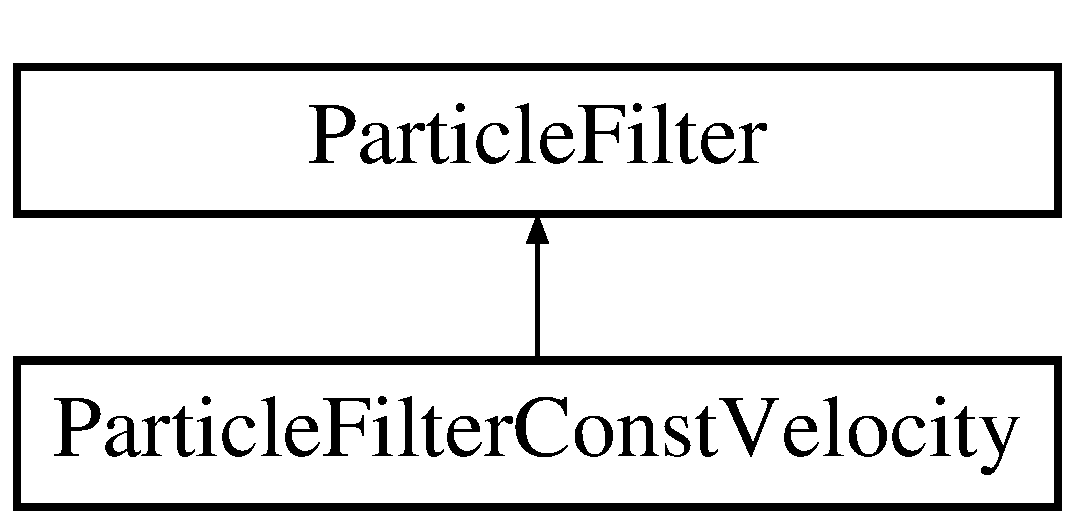
\includegraphics[height=2.000000cm]{classParticleFilterConstVelocity}
\end{center}
\end{figure}
\subsection*{Public Member Functions}
\begin{DoxyCompactItemize}
\item 
\hypertarget{classParticleFilterConstVelocity_a0ae711261a1d992e08de13dac7e2ea70}{}{\bfseries Particle\+Filter\+Const\+Velocity} (int n, float velocity\+Thre, float dist\+Weight)\label{classParticleFilterConstVelocity_a0ae711261a1d992e08de13dac7e2ea70}

\item 
\hypertarget{classParticleFilterConstVelocity_a57692c0a571ab54262e2762469b10b00}{}void {\bfseries Init\+Buffer} ()\label{classParticleFilterConstVelocity_a57692c0a571ab54262e2762469b10b00}

\item 
\hypertarget{classParticleFilterConstVelocity_a3407d048b97f8caebe1353d53f831547}{}void {\bfseries Init\+Target} (const \hyperlink{classRect}{Rect} \&target, const \hyperlink{classPoint2D}{Point2\+D} \&init\+Velocity)\label{classParticleFilterConstVelocity_a3407d048b97f8caebe1353d53f831547}

\item 
\hypertarget{classParticleFilterConstVelocity_a72868ab78e4c4f49ce756e986839f993}{}void {\bfseries Propagate} (const \hyperlink{classSize}{Size} \&img\+Size)\label{classParticleFilterConstVelocity_a72868ab78e4c4f49ce756e986839f993}

\item 
\hypertarget{classParticleFilterConstVelocity_a46aae8bac98e7f6e1f13ad99ec8a38cd}{}void {\bfseries Calculate\+Match\+Score} (const \hyperlink{classIntegralImage}{Integral\+Image} $\ast$int\+Image, const \hyperlink{classStrongClassifier}{Strong\+Classifier} $\ast$classifier, const \hyperlink{classPool}{Pool}$<$ \hyperlink{classRect}{Rect} $>$ \&dets, \hyperlink{classPool}{Pool}$<$ float $>$ \&match\+Array) const \label{classParticleFilterConstVelocity_a46aae8bac98e7f6e1f13ad99ec8a38cd}

\item 
\hypertarget{classParticleFilterConstVelocity_a91f6d8afede8039cd3ed08acbcb67b47}{}void {\bfseries Set\+Velocity\+Sigma} (float sigma)\label{classParticleFilterConstVelocity_a91f6d8afede8039cd3ed08acbcb67b47}

\end{DoxyCompactItemize}
\subsection*{Protected Member Functions}
\begin{DoxyCompactItemize}
\item 
\hypertarget{classParticleFilterConstVelocity_a219193c3bdc2ed042c5473257227c3fb}{}void {\bfseries Init\+Particles} ()\label{classParticleFilterConstVelocity_a219193c3bdc2ed042c5473257227c3fb}

\end{DoxyCompactItemize}
\subsection*{Protected Attributes}
\begin{DoxyCompactItemize}
\item 
\hypertarget{classParticleFilterConstVelocity_af83994fb61bff4a728acced41bdc8cb5}{}\hyperlink{classPoint2D}{Point2\+D} {\bfseries velocity}\label{classParticleFilterConstVelocity_af83994fb61bff4a728acced41bdc8cb5}

\item 
\hypertarget{classParticleFilterConstVelocity_a8e1644ddf56f1c1b20278ca70cdb62ff}{}const float {\bfseries velocity\+Thre}\label{classParticleFilterConstVelocity_a8e1644ddf56f1c1b20278ca70cdb62ff}

\item 
\hypertarget{classParticleFilterConstVelocity_a022c54f062dd30fb21c73945a888b99f}{}const float {\bfseries dist\+Weight}\label{classParticleFilterConstVelocity_a022c54f062dd30fb21c73945a888b99f}

\item 
\hypertarget{classParticleFilterConstVelocity_a4ebdf630669691c8d00fa1f94022921a}{}std\+::normal\+\_\+distribution$<$ float $>$ {\bfseries gaussian\+Velocity}\label{classParticleFilterConstVelocity_a4ebdf630669691c8d00fa1f94022921a}

\end{DoxyCompactItemize}


\subsection{Detailed Description}
\hyperlink{classParticleFilter}{Particle\+Filter} with constant velocity.

\begin{DoxyAuthor}{Author}
Zhengrong Wang. 
\end{DoxyAuthor}


The documentation for this class was generated from the following files\+:\begin{DoxyCompactItemize}
\item 
include/Particle\+Filter\+Const\+Velocity.\+h\item 
src/Particle\+Filter\+Const\+Velocity.\+cpp\end{DoxyCompactItemize}

\hypertarget{classParticleFilterTracker}{}\section{Particle\+Filter\+Tracker Class Reference}
\label{classParticleFilterTracker}\index{Particle\+Filter\+Tracker@{Particle\+Filter\+Tracker}}
Inheritance diagram for Particle\+Filter\+Tracker\+:\begin{figure}[H]
\begin{center}
\leavevmode
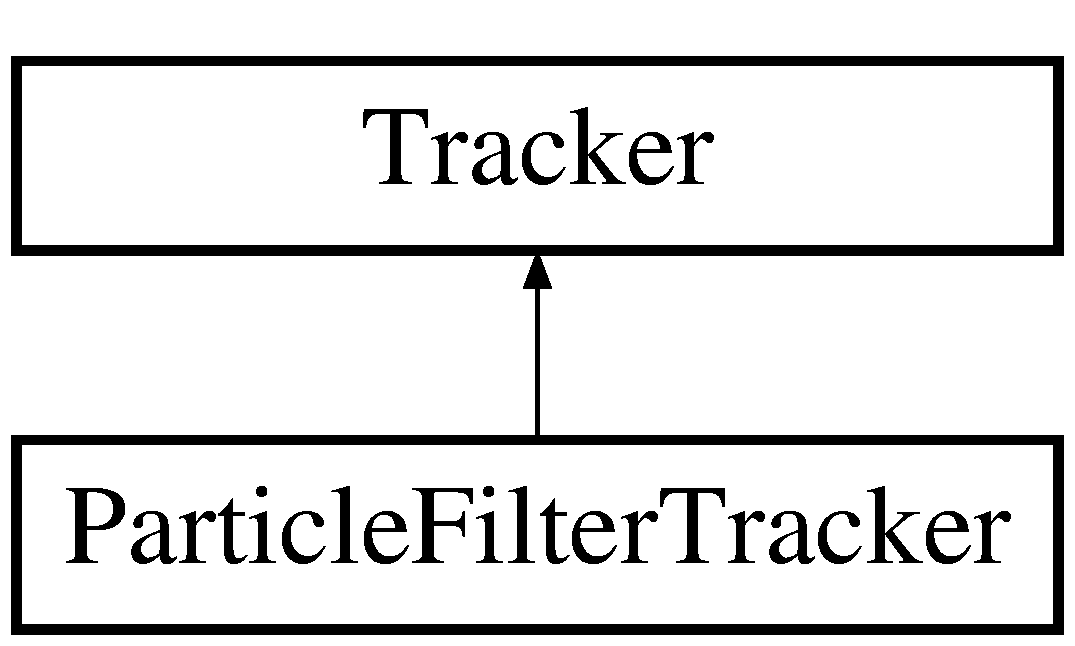
\includegraphics[height=2.000000cm]{classParticleFilterTracker}
\end{center}
\end{figure}
\subsection*{Public Member Functions}
\begin{DoxyCompactItemize}
\item 
\hypertarget{classParticleFilterTracker_ad210c144a99e19d077b4752f78998886}{}{\bfseries Particle\+Filter\+Tracker} (\hyperlink{classStrongClassifier}{Strong\+Classifier} $\ast$classifier, \hyperlink{classIntegralImage}{Integral\+Image} $\ast$int\+Image, \hyperlink{classParticleFilter}{Particle\+Filter} $\ast$particle\+Filter)\label{classParticleFilterTracker_ad210c144a99e19d077b4752f78998886}

\item 
\hypertarget{classParticleFilterTracker_ad19ecb5024b65756896dc53293ea4d56}{}virtual void {\bfseries Track} (cv\+::\+Video\+Capture \&in, cv\+::\+Video\+Writer \&out)\label{classParticleFilterTracker_ad19ecb5024b65756896dc53293ea4d56}

\end{DoxyCompactItemize}
\subsection*{Protected Attributes}
\begin{DoxyCompactItemize}
\item 
\hypertarget{classParticleFilterTracker_ad585da715e3f1711ea1c554ffd94e389}{}\hyperlink{classStrongClassifier}{Strong\+Classifier} $\ast$ {\bfseries classifier}\label{classParticleFilterTracker_ad585da715e3f1711ea1c554ffd94e389}

\item 
\hypertarget{classParticleFilterTracker_abd3719107a5a7594cd90eded262ff246}{}\hyperlink{classIntegralImage}{Integral\+Image} $\ast$ {\bfseries int\+Image}\label{classParticleFilterTracker_abd3719107a5a7594cd90eded262ff246}

\item 
\hypertarget{classParticleFilterTracker_aad6d152590d59bbd7cbd0515a14b3954}{}\hyperlink{classParticleFilter}{Particle\+Filter} $\ast$ {\bfseries particle\+Filter}\label{classParticleFilterTracker_aad6d152590d59bbd7cbd0515a14b3954}

\end{DoxyCompactItemize}


The documentation for this class was generated from the following files\+:\begin{DoxyCompactItemize}
\item 
include/Particle\+Filter\+Tracker.\+h\item 
src/Particle\+Filter\+Tracker.\+cpp\end{DoxyCompactItemize}

\hypertarget{classPoint2D}{}\section{Point2\+D Class Reference}
\label{classPoint2D}\index{Point2\+D@{Point2\+D}}
\subsection*{Public Member Functions}
\begin{DoxyCompactItemize}
\item 
\hypertarget{classPoint2D_ab6b269e58cadf99c3b290a43e04c9576}{}{\bfseries Point2\+D} (int r=0, int c=0)\label{classPoint2D_ab6b269e58cadf99c3b290a43e04c9576}

\item 
\hypertarget{classPoint2D_ab91688dc27a2072ab3efaf068c7a57e0}{}\hyperlink{classPoint2D}{Point2\+D} \& {\bfseries operator=} (const \hyperlink{classRect}{Rect} \&r)\label{classPoint2D_ab91688dc27a2072ab3efaf068c7a57e0}

\item 
\hypertarget{classPoint2D_a05def5ae8c585b81abacbbfab95ced7d}{}float {\bfseries Squared\+Distance} (const \hyperlink{classPoint2D}{Point2\+D} \&other) const \label{classPoint2D_a05def5ae8c585b81abacbbfab95ced7d}

\item 
\hypertarget{classPoint2D_a53134a6fffd5af2cc0e94267b1c50f4e}{}float {\bfseries Distance} (const \hyperlink{classPoint2D}{Point2\+D} \&other) const \label{classPoint2D_a53134a6fffd5af2cc0e94267b1c50f4e}

\end{DoxyCompactItemize}
\subsection*{Public Attributes}
\begin{DoxyCompactItemize}
\item 
\hypertarget{classPoint2D_ab2066342cc783a1ff0f0cf0e8357138a}{}int {\bfseries row}\label{classPoint2D_ab2066342cc783a1ff0f0cf0e8357138a}

\item 
\hypertarget{classPoint2D_af5f355c29cdbafa6e446208824a77b19}{}int {\bfseries col}\label{classPoint2D_af5f355c29cdbafa6e446208824a77b19}

\end{DoxyCompactItemize}


The documentation for this class was generated from the following files\+:\begin{DoxyCompactItemize}
\item 
include/Geometry.\+h\item 
src/Geometry.\+cpp\end{DoxyCompactItemize}

\hypertarget{classPool}{}\section{Pool$<$ T $>$ Class Template Reference}
\label{classPool}\index{Pool$<$ T $>$@{Pool$<$ T $>$}}


{\ttfamily \#include $<$Pool.\+h$>$}

\subsection*{Public Member Functions}
\begin{DoxyCompactItemize}
\item 
\hypertarget{classPool_ac4076ad218acab283dacc29e8e2cf855}{}T \& {\bfseries operator\mbox{[}$\,$\mbox{]}} (uint index)\label{classPool_ac4076ad218acab283dacc29e8e2cf855}

\item 
\hypertarget{classPool_acbec03f17980c373ecf27ed2db420d7b}{}void {\bfseries Push} (const T \&t)\label{classPool_acbec03f17980c373ecf27ed2db420d7b}

\item 
\hypertarget{classPool_aae8e8528b907d7339af05685ba49aa92}{}void {\bfseries clear} ()\label{classPool_aae8e8528b907d7339af05685ba49aa92}

\end{DoxyCompactItemize}
\subsection*{Public Attributes}
\begin{DoxyCompactItemize}
\item 
\hypertarget{classPool_a2c33796e829a9c6d536a85b7ad62d309}{}int {\bfseries size}\label{classPool_a2c33796e829a9c6d536a85b7ad62d309}

\item 
\hypertarget{classPool_a9a3a4597a8e96a97b2186f972104f196}{}std\+::vector$<$ T $>$ {\bfseries data}\label{classPool_a9a3a4597a8e96a97b2186f972104f196}

\end{DoxyCompactItemize}


\subsection{Detailed Description}
\subsubsection*{template$<$typename T$>$class Pool$<$ T $>$}

Use std\+::vector as the container, however it never shrinks. \begin{DoxyAuthor}{Author}
Zhengrong Wang. 
\end{DoxyAuthor}


The documentation for this class was generated from the following file\+:\begin{DoxyCompactItemize}
\item 
include/Pool.\+h\end{DoxyCompactItemize}

\hypertarget{structrect}{}\section{rect Struct Reference}
\label{structrect}\index{rect@{rect}}


{\ttfamily \#include $<$Image\+Detector.\+h$>$}

\subsection*{Public Member Functions}
\begin{DoxyCompactItemize}
\item 
\hypertarget{structrect_ac4d3220b8b456e1ba3a17ce1c3c8dd9e}{}{\bfseries rect} (int \+\_\+x1=0, int \+\_\+y1=0, int \+\_\+x2=0, int \+\_\+y2=0)\label{structrect_ac4d3220b8b456e1ba3a17ce1c3c8dd9e}

\end{DoxyCompactItemize}
\subsection*{Public Attributes}
\begin{DoxyCompactItemize}
\item 
\hypertarget{structrect_a69beca6e9401efeab8da0cd15e98b3e6}{}int {\bfseries x1}\label{structrect_a69beca6e9401efeab8da0cd15e98b3e6}

\item 
\hypertarget{structrect_adfb4f185d1c0793506fb29fd553d42b5}{}int {\bfseries y1}\label{structrect_adfb4f185d1c0793506fb29fd553d42b5}

\item 
\hypertarget{structrect_a282dd568f7f09097b0d04d14e8bcd65c}{}int {\bfseries x2}\label{structrect_a282dd568f7f09097b0d04d14e8bcd65c}

\item 
\hypertarget{structrect_a7bffd714159408a1597411ebf9b937d1}{}int {\bfseries y2}\label{structrect_a7bffd714159408a1597411ebf9b937d1}

\item 
\hypertarget{structrect_abef077625c66b02797d2263e824d82b7}{}int {\bfseries re}\label{structrect_abef077625c66b02797d2263e824d82b7}

\item 
\hypertarget{structrect_a717f683ace299d924821febb664eaef0}{}int {\bfseries count}\label{structrect_a717f683ace299d924821febb664eaef0}

\end{DoxyCompactItemize}


\subsection{Detailed Description}
There are basically two kinds of detectors. \hyperlink{classImageDetector}{Image\+Detector}\+: detects pedestrains in an image. \hyperlink{classVideoDetector}{Video\+Detector}\+: detects pedestrains in a video. 

The documentation for this struct was generated from the following file\+:\begin{DoxyCompactItemize}
\item 
include/Image\+Detector.\+h\end{DoxyCompactItemize}

\hypertarget{classRect}{}\section{Rect Class Reference}
\label{classRect}\index{Rect@{Rect}}
\subsection*{Public Member Functions}
\begin{DoxyCompactItemize}
\item 
\hypertarget{classRect_ad197c38803bb8538dd04e5a92b5e12e6}{}{\bfseries Rect} (int u=0, int l=0, int w=0, int h=0)\label{classRect_ad197c38803bb8538dd04e5a92b5e12e6}

\item 
\hypertarget{classRect_a7fbb8992edb8c3839c83045213d21631}{}\hyperlink{classRect}{Rect} {\bfseries operator+} (const \hyperlink{classPoint2D}{Point2\+D} \&offset) const \label{classRect_a7fbb8992edb8c3839c83045213d21631}

\item 
\hypertarget{classRect_a90d8491cab865d559ccb00fe88027714}{}bool {\bfseries Is\+Overlap} (const \hyperlink{classRect}{Rect} \&other) const \label{classRect_a90d8491cab865d559ccb00fe88027714}

\item 
bool \hyperlink{classRect_a3ab55f8bbc938075ff7a23fb95bfdd26}{Is\+In} (const \hyperlink{classRect}{Rect} \&other) const 
\item 
\hypertarget{classRect_afb25e86036b7faa93e86aee8ba24cd35}{}{\bfseries operator cv\+::\+Rect} () const \label{classRect_afb25e86036b7faa93e86aee8ba24cd35}

\item 
\hypertarget{classRect_a78ef656476b85aa5ba0f8dd70a6232d3}{}{\bfseries operator Size} () const \label{classRect_a78ef656476b85aa5ba0f8dd70a6232d3}

\end{DoxyCompactItemize}
\subsection*{Public Attributes}
\begin{DoxyCompactItemize}
\item 
\hypertarget{classRect_aaba0474a7052cee8cadd159c306e27bd}{}int {\bfseries upper}\label{classRect_aaba0474a7052cee8cadd159c306e27bd}

\item 
\hypertarget{classRect_ab0841a51d249d8560ddca36054fd1e57}{}int {\bfseries left}\label{classRect_ab0841a51d249d8560ddca36054fd1e57}

\item 
\hypertarget{classRect_ad79d7bf12771a81627a672452437011d}{}int {\bfseries height}\label{classRect_ad79d7bf12771a81627a672452437011d}

\item 
\hypertarget{classRect_a367714e71d566668addb140c7981b5bc}{}int {\bfseries width}\label{classRect_a367714e71d566668addb140c7981b5bc}

\end{DoxyCompactItemize}


\subsection{Member Function Documentation}
\hypertarget{classRect_a3ab55f8bbc938075ff7a23fb95bfdd26}{}\index{Rect@{Rect}!Is\+In@{Is\+In}}
\index{Is\+In@{Is\+In}!Rect@{Rect}}
\subsubsection[{Is\+In(const Rect \&other) const }]{\setlength{\rightskip}{0pt plus 5cm}bool Rect\+::\+Is\+In (
\begin{DoxyParamCaption}
\item[{const {\bf Rect} \&}]{other}
\end{DoxyParamCaption}
) const\hspace{0.3cm}{\ttfamily [inline]}}\label{classRect_a3ab55f8bbc938075ff7a23fb95bfdd26}
Is the other rectangle all inside this one. 

The documentation for this class was generated from the following files\+:\begin{DoxyCompactItemize}
\item 
include/Geometry.\+h\item 
src/Geometry.\+cpp\end{DoxyCompactItemize}

\hypertarget{classRGIFeature}{}\section{R\+G\+I\+Feature Class Reference}
\label{classRGIFeature}\index{R\+G\+I\+Feature@{R\+G\+I\+Feature}}
\subsection*{Public Member Functions}
\begin{DoxyCompactItemize}
\item 
\hypertarget{classRGIFeature_ad6aae4be82bd6f86d21675453983ff7d}{}{\bfseries R\+G\+I\+Feature} (const \hyperlink{classSize}{Size} \&patch\+Size)\label{classRGIFeature_ad6aae4be82bd6f86d21675453983ff7d}

\item 
\hypertarget{classRGIFeature_a82a0aa084cb027d6ea68a90460a633b7}{}void {\bfseries Get\+Initial\+Distribution} (\hyperlink{classEstimatedGaussianDistribution}{Estimated\+Gaussian\+Distribution}$<$ N\+U\+M\+\_\+\+R\+G\+I\+\_\+\+B\+I\+N\+S $>$ $\ast$distribution) const \label{classRGIFeature_a82a0aa084cb027d6ea68a90460a633b7}

\item 
\hypertarget{classRGIFeature_a603a11aa48dd81f4c7f867662587b30c}{}bool {\bfseries Extract} (const \hyperlink{classIntegralImage}{Integral\+Image} $\ast$int\+Image, const \hyperlink{classRect}{Rect} \&roi, \hyperlink{classFeature}{Feature} $\ast$feature)\label{classRGIFeature_a603a11aa48dd81f4c7f867662587b30c}

\end{DoxyCompactItemize}


The documentation for this class was generated from the following files\+:\begin{DoxyCompactItemize}
\item 
include/R\+G\+I\+Feature.\+h\item 
src/R\+G\+I\+Feature.\+cpp\end{DoxyCompactItemize}

\hypertarget{classRGIIntegralImage}{}\section{R\+G\+I\+Integral\+Image Class Reference}
\label{classRGIIntegralImage}\index{R\+G\+I\+Integral\+Image@{R\+G\+I\+Integral\+Image}}
Inheritance diagram for R\+G\+I\+Integral\+Image\+:\begin{figure}[H]
\begin{center}
\leavevmode
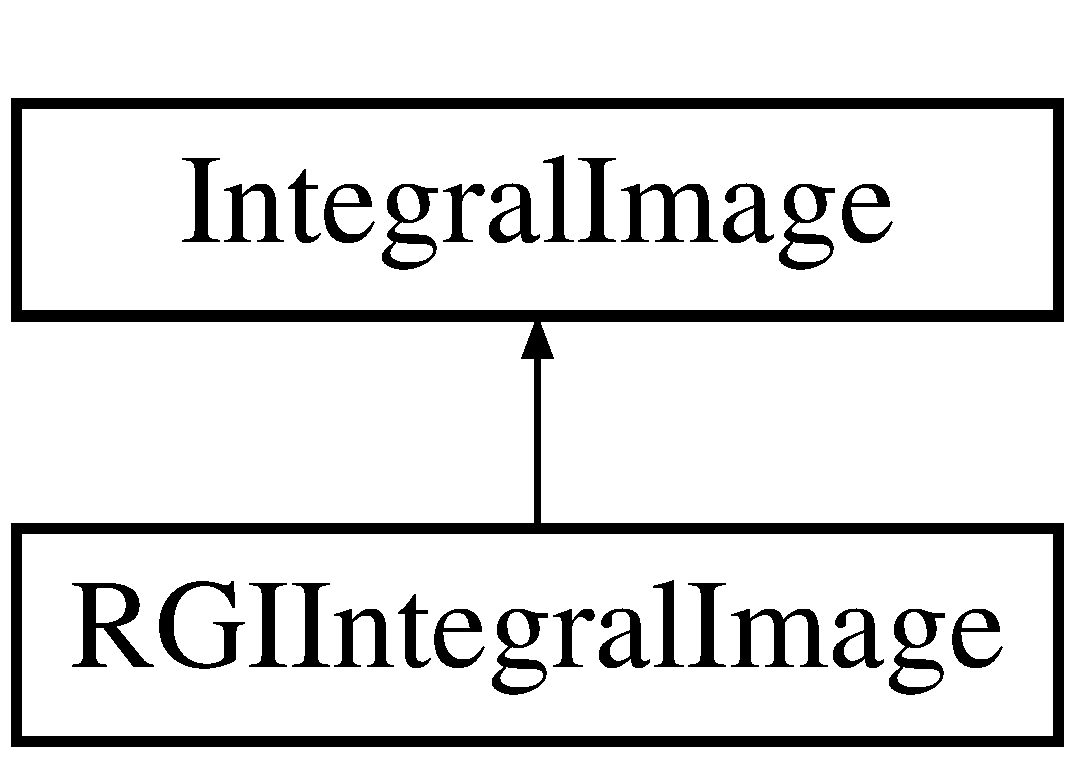
\includegraphics[height=2.000000cm]{classRGIIntegralImage}
\end{center}
\end{figure}
\subsection*{Public Member Functions}
\begin{DoxyCompactItemize}
\item 
\hyperlink{classRGIIntegralImage_ab1974df4946fd93d55ada1a09e91945e}{R\+G\+I\+Integral\+Image} (const cv\+::\+Mat \&img)
\item 
\hypertarget{classRGIIntegralImage_ac98031658bec86c125687fdaf91c8ecd}{}{\bfseries R\+G\+I\+Integral\+Image} (int w, int h)\label{classRGIIntegralImage_ac98031658bec86c125687fdaf91c8ecd}

\item 
\hypertarget{classRGIIntegralImage_a72924e4bd0b101b8b3a38202641b3ba3}{}void {\bfseries Calculate\+Int} (const cv\+::\+Mat \&img)\label{classRGIIntegralImage_a72924e4bd0b101b8b3a38202641b3ba3}

\item 
\hypertarget{classRGIIntegralImage_aad51158989b50545304e4db71144c49a}{}void {\bfseries Get\+Sum} (const \hyperlink{classRect}{Rect} \&roi, float $\ast$result) const \label{classRGIIntegralImage_aad51158989b50545304e4db71144c49a}

\end{DoxyCompactItemize}
\subsection*{Additional Inherited Members}


\subsection{Constructor \& Destructor Documentation}
\hypertarget{classRGIIntegralImage_ab1974df4946fd93d55ada1a09e91945e}{}\index{R\+G\+I\+Integral\+Image@{R\+G\+I\+Integral\+Image}!R\+G\+I\+Integral\+Image@{R\+G\+I\+Integral\+Image}}
\index{R\+G\+I\+Integral\+Image@{R\+G\+I\+Integral\+Image}!R\+G\+I\+Integral\+Image@{R\+G\+I\+Integral\+Image}}
\subsubsection[{R\+G\+I\+Integral\+Image(const cv\+::\+Mat \&img)}]{\setlength{\rightskip}{0pt plus 5cm}R\+G\+I\+Integral\+Image\+::\+R\+G\+I\+Integral\+Image (
\begin{DoxyParamCaption}
\item[{const cv\+::\+Mat \&}]{img}
\end{DoxyParamCaption}
)}\label{classRGIIntegralImage_ab1974df4946fd93d55ada1a09e91945e}

\begin{DoxyParams}{Parameters}
{\em img} & should be 8\+U\+C3, e.\+g. R\+G\+B image. \\
\hline
\end{DoxyParams}


The documentation for this class was generated from the following files\+:\begin{DoxyCompactItemize}
\item 
include/R\+G\+I\+Integral\+Image.\+h\item 
src/R\+G\+I\+Integral\+Image.\+cpp\end{DoxyCompactItemize}

\hypertarget{structrow__data}{}\section{row\+\_\+data Struct Reference}
\label{structrow__data}\index{row\+\_\+data@{row\+\_\+data}}
\subsection*{Public Attributes}
\begin{DoxyCompactItemize}
\item 
\hypertarget{structrow__data_ad8f2f35f7df63f710653639dfb6d4ad8}{}double {\bfseries row}\label{structrow__data_ad8f2f35f7df63f710653639dfb6d4ad8}

\item 
\hypertarget{structrow__data_ad9ca787aa08dfb3a1a38bc903068f2ad}{}int {\bfseries label}\label{structrow__data_ad9ca787aa08dfb3a1a38bc903068f2ad}

\end{DoxyCompactItemize}


The documentation for this struct was generated from the following file\+:\begin{DoxyCompactItemize}
\item 
include/kmeans.\+h\end{DoxyCompactItemize}

\hypertarget{classSingleSampler}{}\section{Single\+Sampler Class Reference}
\label{classSingleSampler}\index{Single\+Sampler@{Single\+Sampler}}


{\ttfamily \#include $<$Single\+Sampler.\+h$>$}

\subsection*{Public Member Functions}
\begin{DoxyCompactItemize}
\item 
\hypertarget{classSingleSampler_ac8afcdb74dfa26de9e686879eb2062fd}{}{\bfseries Single\+Sampler} (int num\+Pos, int num\+Neg)\label{classSingleSampler_ac8afcdb74dfa26de9e686879eb2062fd}

\item 
\hypertarget{classSingleSampler_aea28b8157e66fff3bf2d919638d6bf8f}{}int {\bfseries Get\+Num\+Pos} () const \label{classSingleSampler_aea28b8157e66fff3bf2d919638d6bf8f}

\item 
\hypertarget{classSingleSampler_a2c615500fb49179a6a7ab606e19d5438}{}int {\bfseries Get\+Num\+Neg} () const \label{classSingleSampler_a2c615500fb49179a6a7ab606e19d5438}

\item 
\hypertarget{classSingleSampler_a5cd8387d318cfa166763efa601c6a016}{}const \hyperlink{classRect}{Rect} \& {\bfseries Get\+Pos\+Sample} (int index) const \label{classSingleSampler_a5cd8387d318cfa166763efa601c6a016}

\item 
\hypertarget{classSingleSampler_a5b07ba58d23e251a745752185d474995}{}const \hyperlink{classRect}{Rect} \& {\bfseries Get\+Neg\+Sample} (int index) const \label{classSingleSampler_a5b07ba58d23e251a745752185d474995}

\item 
\hypertarget{classSingleSampler_a0211ef10f190b5b9e56a7103e8437b19}{}virtual void {\bfseries Sample} (const \hyperlink{classRect}{Rect} \&pos, const \hyperlink{classSize}{Size} \&img\+Size)\label{classSingleSampler_a0211ef10f190b5b9e56a7103e8437b19}

\item 
\hypertarget{classSingleSampler_a38a0df4f2d8d190708921df130c6fbb1}{}void {\bfseries Draw\+Samples} (cv\+::\+Mat \&img, const cv\+::\+Scalar \&pos\+Color, const cv\+::\+Scalar \&neg\+Color) const \label{classSingleSampler_a38a0df4f2d8d190708921df130c6fbb1}

\item 
void \hyperlink{classSingleSampler_a8be19d5fe2cba8f042835df152e2e4d4}{Draw\+Sample} (cv\+::\+Mat \&img, const cv\+::\+Scalar \&color, int index=0, int target=1) const 
\end{DoxyCompactItemize}
\subsection*{Protected Attributes}
\begin{DoxyCompactItemize}
\item 
\hypertarget{classSingleSampler_aae910dbaf3271e79601e9e4c786eaad1}{}int {\bfseries num\+Neg\+Samples}\label{classSingleSampler_aae910dbaf3271e79601e9e4c786eaad1}

\item 
\hypertarget{classSingleSampler_a9a624f9a0519802d38fa760578e43ce2}{}int {\bfseries num\+Pos\+Samples}\label{classSingleSampler_a9a624f9a0519802d38fa760578e43ce2}

\item 
\hypertarget{classSingleSampler_add879b72a8fb9bc537b2c73def6b4ab4}{}\hyperlink{classRect}{Rect} $\ast$ {\bfseries neg\+Samples}\label{classSingleSampler_add879b72a8fb9bc537b2c73def6b4ab4}

\item 
\hypertarget{classSingleSampler_a66244f71e586f614b1f505cfa74034bf}{}\hyperlink{classRect}{Rect} $\ast$ {\bfseries pos\+Samples}\label{classSingleSampler_a66244f71e586f614b1f505cfa74034bf}

\item 
\hypertarget{classSingleSampler_a584faf8d63d5985a64f7eb1f560b501c}{}int {\bfseries cur\+Pos\+Sample}\label{classSingleSampler_a584faf8d63d5985a64f7eb1f560b501c}

\item 
\hypertarget{classSingleSampler_a9ed280c3389a16c34a7e7ba97150d2c1}{}int {\bfseries cur\+Neg\+Sample}\label{classSingleSampler_a9ed280c3389a16c34a7e7ba97150d2c1}

\item 
\hypertarget{classSingleSampler_af5aa1a24a704f7b553b40c846d7425fd}{}std\+::normal\+\_\+distribution$<$ float $>$ {\bfseries gaussian\+Width}\label{classSingleSampler_af5aa1a24a704f7b553b40c846d7425fd}

\item 
\hypertarget{classSingleSampler_ae8dc991f539b05c59884da2107b2cedb}{}std\+::normal\+\_\+distribution$<$ float $>$ {\bfseries gaussian\+Height}\label{classSingleSampler_ae8dc991f539b05c59884da2107b2cedb}

\end{DoxyCompactItemize}
\subsection*{Static Protected Attributes}
\begin{DoxyCompactItemize}
\item 
\hypertarget{classSingleSampler_a54b9846441e263f759935b621a89cadc}{}static std\+::default\+\_\+random\+\_\+engine {\bfseries generator}\label{classSingleSampler_a54b9846441e263f759935b621a89cadc}

\end{DoxyCompactItemize}


\subsection{Detailed Description}
Sampler interface. This is used to sample neg and pos examples. Given a positive sample, it samples num\+Neg\+Samples negative samples around it. \begin{DoxyAuthor}{Author}
Zhengrong Wang, Hsienyu Meng. 
\end{DoxyAuthor}


\subsection{Member Function Documentation}
\hypertarget{classSingleSampler_a8be19d5fe2cba8f042835df152e2e4d4}{}\index{Single\+Sampler@{Single\+Sampler}!Draw\+Sample@{Draw\+Sample}}
\index{Draw\+Sample@{Draw\+Sample}!Single\+Sampler@{Single\+Sampler}}
\subsubsection[{Draw\+Sample(cv\+::\+Mat \&img, const cv\+::\+Scalar \&color, int index=0, int target=1) const }]{\setlength{\rightskip}{0pt plus 5cm}void Single\+Sampler\+::\+Draw\+Sample (
\begin{DoxyParamCaption}
\item[{cv\+::\+Mat \&}]{img, }
\item[{const cv\+::\+Scalar \&}]{color, }
\item[{int}]{index = {\ttfamily 0}, }
\item[{int}]{target = {\ttfamily 1}}
\end{DoxyParamCaption}
) const}\label{classSingleSampler_a8be19d5fe2cba8f042835df152e2e4d4}
Draw a specific sample.


\begin{DoxyParams}{Parameters}
{\em img} & the image to draw \\
\hline
{\em color} & color we will use \\
\hline
{\em index} & the index of the sample \\
\hline
{\em target} & positive or negative samples \\
\hline
\end{DoxyParams}


The documentation for this class was generated from the following files\+:\begin{DoxyCompactItemize}
\item 
include/Single\+Sampler.\+h\item 
src/Single\+Sampler.\+cpp\end{DoxyCompactItemize}

\hypertarget{classSingleTarget}{}\section{Single\+Target Class Reference}
\label{classSingleTarget}\index{Single\+Target@{Single\+Target}}


{\ttfamily \#include $<$Single\+Target.\+h$>$}

\subsection*{Public Member Functions}
\begin{DoxyCompactItemize}
\item 
\hyperlink{classSingleTarget_a0f9683df9354a8256f622db973130833}{Single\+Target} (const \hyperlink{structOptions}{Options} \&ops)
\item 
\hypertarget{classSingleTarget_afa791ad34c84b8a9d9d2e60398e5db2e}{}void {\bfseries Initialize\+Target} (const \hyperlink{classRect}{Rect} \&target, const \hyperlink{classPoint2D}{Point2\+D} \&init\+Velocity)\label{classSingleTarget_afa791ad34c84b8a9d9d2e60398e5db2e}

\item 
void \hyperlink{classSingleTarget_a2036d90f89d1a65966523c559aee3d38}{Propagate} (const \hyperlink{classSize}{Size} \&img\+Size)
\item 
void \hyperlink{classSingleTarget_a9ce84c111efa084c8bf9aa89736dffc8}{Observe} (const \hyperlink{classIntegralImage}{Integral\+Image} $\ast$int\+Image, const \hyperlink{classRect}{Rect} \&detection, float detection\+Weight)
\item 
void \hyperlink{classSingleTarget_a1e22348deeeae3e5d8d1c964df9c8fc8}{Observe} (const \hyperlink{classIntegralImage}{Integral\+Image} $\ast$int\+Image)
\item 
void \hyperlink{classSingleTarget_a5b2d2b9313f7d3bd8d96af68f840bff4}{Update} (const \hyperlink{classIntegralImage}{Integral\+Image} $\ast$int\+Image, const \hyperlink{classRect}{Rect} \&roi, int target, float importance=1.\+0f)
\item 
void \hyperlink{classSingleTarget_a450151cccff458e3603a34c99ccd4134}{Calculate\+Match\+Score} (const \hyperlink{classIntegralImage}{Integral\+Image} $\ast$int\+Image, const \hyperlink{classPool}{Pool}$<$ \hyperlink{classRect}{Rect} $>$ \&dets, \hyperlink{classPool}{Pool}$<$ float $>$ \&match\+Array) const 
\item 
void \hyperlink{classSingleTarget_aa620ca1f64fe972c8dc110e0a6012213}{Update\+Seq} (bool is\+Detected)
\item 
\hypertarget{classSingleTarget_a4b77b8dbe78d051ab5f190eef5b9a51a}{}void {\bfseries Resample\+With\+Best} ()\label{classSingleTarget_a4b77b8dbe78d051ab5f190eef5b9a51a}

\item 
\hypertarget{classSingleTarget_a8ba04565921bcbcce7a04c1c76daa4ca}{}void {\bfseries Resample\+With\+Confidence} ()\label{classSingleTarget_a8ba04565921bcbcce7a04c1c76daa4ca}

\end{DoxyCompactItemize}


\subsection{Detailed Description}
Parameters for an empty target.


\begin{DoxyParams}{Parameters}
{\em n\+Particles} & \# particles \\
\hline
{\em target} & the target region \\
\hline
{\em init\+Velocity} & the initial velocity \\
\hline
{\em num\+Selectors} & \# selectors in strong classifier \\
\hline
{\em num\+Weak\+Classifiers} & \# weak classifiers \\
\hline
{\em num\+Backups} & \# backup weak classifiers \\
\hline
{\em dist\+Weight} & distance weight for match score \\
\hline
{\em velocity\+Thre} & velocity threshold for match score \\
\hline
{\em velocity\+Sigma\+Const} & const number for velocity sigma \\
\hline
\end{DoxyParams}


\subsection{Constructor \& Destructor Documentation}
\hypertarget{classSingleTarget_a0f9683df9354a8256f622db973130833}{}\index{Single\+Target@{Single\+Target}!Single\+Target@{Single\+Target}}
\index{Single\+Target@{Single\+Target}!Single\+Target@{Single\+Target}}
\subsubsection[{Single\+Target(const Options \&ops)}]{\setlength{\rightskip}{0pt plus 5cm}Single\+Target\+::\+Single\+Target (
\begin{DoxyParamCaption}
\item[{const {\bf Options} \&}]{ops}
\end{DoxyParamCaption}
)}\label{classSingleTarget_a0f9683df9354a8256f622db973130833}
Construct an empty target. 

\subsection{Member Function Documentation}
\hypertarget{classSingleTarget_a450151cccff458e3603a34c99ccd4134}{}\index{Single\+Target@{Single\+Target}!Calculate\+Match\+Score@{Calculate\+Match\+Score}}
\index{Calculate\+Match\+Score@{Calculate\+Match\+Score}!Single\+Target@{Single\+Target}}
\subsubsection[{Calculate\+Match\+Score(const Integral\+Image $\ast$int\+Image, const Pool$<$ Rect $>$ \&dets, Pool$<$ float $>$ \&match\+Array) const }]{\setlength{\rightskip}{0pt plus 5cm}void Single\+Target\+::\+Calculate\+Match\+Score (
\begin{DoxyParamCaption}
\item[{const {\bf Integral\+Image} $\ast$}]{int\+Image, }
\item[{const {\bf Pool}$<$ {\bf Rect} $>$ \&}]{dets, }
\item[{{\bf Pool}$<$ float $>$ \&}]{match\+Array}
\end{DoxyParamCaption}
) const}\label{classSingleTarget_a450151cccff458e3603a34c99ccd4134}
Calculate the match score with all the detections.


\begin{DoxyParams}{Parameters}
{\em int\+Image} & in\+: integral image \\
\hline
{\em dets} & in\+: detections \\
\hline
{\em march\+Array} & out\+: the match score \\
\hline
\end{DoxyParams}
\hypertarget{classSingleTarget_a9ce84c111efa084c8bf9aa89736dffc8}{}\index{Single\+Target@{Single\+Target}!Observe@{Observe}}
\index{Observe@{Observe}!Single\+Target@{Single\+Target}}
\subsubsection[{Observe(const Integral\+Image $\ast$int\+Image, const Rect \&detection, float detection\+Weight)}]{\setlength{\rightskip}{0pt plus 5cm}void Single\+Target\+::\+Observe (
\begin{DoxyParamCaption}
\item[{const {\bf Integral\+Image} $\ast$}]{int\+Image, }
\item[{const {\bf Rect} \&}]{detection, }
\item[{float}]{detection\+Weight}
\end{DoxyParamCaption}
)\hspace{0.3cm}{\ttfamily [inline]}}\label{classSingleTarget_a9ce84c111efa084c8bf9aa89736dffc8}
Observe the particles. weight\+\_\+particle = detection\+Weight $\ast$ P(particle, detection) + (1.\+0f -\/ detection\+Weight) $\ast$ Conf(particle)


\begin{DoxyParams}{Parameters}
{\em detection} & The associate detection, if any. \\
\hline
{\em detection\+Weight} & weight for detection term \\
\hline
{\em classifier\+Weight} & weight for classifier term \\
\hline
\end{DoxyParams}
\hypertarget{classSingleTarget_a1e22348deeeae3e5d8d1c964df9c8fc8}{}\index{Single\+Target@{Single\+Target}!Observe@{Observe}}
\index{Observe@{Observe}!Single\+Target@{Single\+Target}}
\subsubsection[{Observe(const Integral\+Image $\ast$int\+Image)}]{\setlength{\rightskip}{0pt plus 5cm}void Single\+Target\+::\+Observe (
\begin{DoxyParamCaption}
\item[{const {\bf Integral\+Image} $\ast$}]{int\+Image}
\end{DoxyParamCaption}
)\hspace{0.3cm}{\ttfamily [inline]}}\label{classSingleTarget_a1e22348deeeae3e5d8d1c964df9c8fc8}
Observe the particles without matched detections. \hypertarget{classSingleTarget_a2036d90f89d1a65966523c559aee3d38}{}\index{Single\+Target@{Single\+Target}!Propagate@{Propagate}}
\index{Propagate@{Propagate}!Single\+Target@{Single\+Target}}
\subsubsection[{Propagate(const Size \&img\+Size)}]{\setlength{\rightskip}{0pt plus 5cm}void Single\+Target\+::\+Propagate (
\begin{DoxyParamCaption}
\item[{const {\bf Size} \&}]{img\+Size}
\end{DoxyParamCaption}
)}\label{classSingleTarget_a2036d90f89d1a65966523c559aee3d38}
Propagate the particles. It sets the sigma for velocity and then call \hyperlink{classParticleFilter_a166db9f33feabf14126df2de541a593d}{Particle\+Filter\+::\+Propagate}. \hypertarget{classSingleTarget_a5b2d2b9313f7d3bd8d96af68f840bff4}{}\index{Single\+Target@{Single\+Target}!Update@{Update}}
\index{Update@{Update}!Single\+Target@{Single\+Target}}
\subsubsection[{Update(const Integral\+Image $\ast$int\+Image, const Rect \&roi, int target, float importance=1.\+0f)}]{\setlength{\rightskip}{0pt plus 5cm}void Single\+Target\+::\+Update (
\begin{DoxyParamCaption}
\item[{const {\bf Integral\+Image} $\ast$}]{int\+Image, }
\item[{const {\bf Rect} \&}]{roi, }
\item[{int}]{target, }
\item[{float}]{importance = {\ttfamily 1.0f}}
\end{DoxyParamCaption}
)}\label{classSingleTarget_a5b2d2b9313f7d3bd8d96af68f840bff4}
Update the classifier. Only used when there are no overlapping detection and we are damn sure this is the correct one. \hypertarget{classSingleTarget_aa620ca1f64fe972c8dc110e0a6012213}{}\index{Single\+Target@{Single\+Target}!Update\+Seq@{Update\+Seq}}
\index{Update\+Seq@{Update\+Seq}!Single\+Target@{Single\+Target}}
\subsubsection[{Update\+Seq(bool is\+Detected)}]{\setlength{\rightskip}{0pt plus 5cm}void Single\+Target\+::\+Update\+Seq (
\begin{DoxyParamCaption}
\item[{bool}]{is\+Detected}
\end{DoxyParamCaption}
)\hspace{0.3cm}{\ttfamily [inline]}}\label{classSingleTarget_aa620ca1f64fe972c8dc110e0a6012213}
Update the detection sequence. 

The documentation for this class was generated from the following files\+:\begin{DoxyCompactItemize}
\item 
include/Single\+Target.\+h\item 
src/Single\+Target.\+cpp\end{DoxyCompactItemize}

\hypertarget{classSize}{}\section{Size Class Reference}
\label{classSize}\index{Size@{Size}}
\subsection*{Public Member Functions}
\begin{DoxyCompactItemize}
\item 
\hypertarget{classSize_a0ea0a7599bb78efd82b1a15d2bf99949}{}{\bfseries Size} (int w=0, int h=0)\label{classSize_a0ea0a7599bb78efd82b1a15d2bf99949}

\item 
\hypertarget{classSize_a1afcc84f430e6034f296f0b167f76d51}{}\hyperlink{classSize}{Size} {\bfseries operator=} (const \hyperlink{classRect}{Rect} \&r)\label{classSize_a1afcc84f430e6034f296f0b167f76d51}

\item 
\hypertarget{classSize_ac806d63f500f065ce5eddfaaf8b0bb07}{}\hyperlink{classSize}{Size} {\bfseries operator$\ast$} (float f)\label{classSize_ac806d63f500f065ce5eddfaaf8b0bb07}

\item 
\hypertarget{classSize_a11cb27cff6cc1767a76fec0e1f5dd4d2}{}bool {\bfseries operator==} (const \hyperlink{classSize}{Size} \&other) const \label{classSize_a11cb27cff6cc1767a76fec0e1f5dd4d2}

\end{DoxyCompactItemize}
\subsection*{Public Attributes}
\begin{DoxyCompactItemize}
\item 
\hypertarget{classSize_aa1f23158085de487cfd5434301c077a4}{}int {\bfseries width}\label{classSize_aa1f23158085de487cfd5434301c077a4}

\item 
\hypertarget{classSize_a4cdfe2d67b3f87b3f5d86bfafd5df036}{}int {\bfseries height}\label{classSize_a4cdfe2d67b3f87b3f5d86bfafd5df036}

\item 
\hypertarget{classSize_a9603965bb9c8fd9fc0ae651412b2a3e0}{}int {\bfseries area}\label{classSize_a9603965bb9c8fd9fc0ae651412b2a3e0}

\end{DoxyCompactItemize}


The documentation for this class was generated from the following files\+:\begin{DoxyCompactItemize}
\item 
include/Geometry.\+h\item 
src/Geometry.\+cpp\end{DoxyCompactItemize}

\hypertarget{classStrongClassifier}{}\section{Strong\+Classifier Class Reference}
\label{classStrongClassifier}\index{Strong\+Classifier@{Strong\+Classifier}}


{\ttfamily \#include $<$Strong\+Classifier.\+h$>$}

Inheritance diagram for Strong\+Classifier\+:\begin{figure}[H]
\begin{center}
\leavevmode
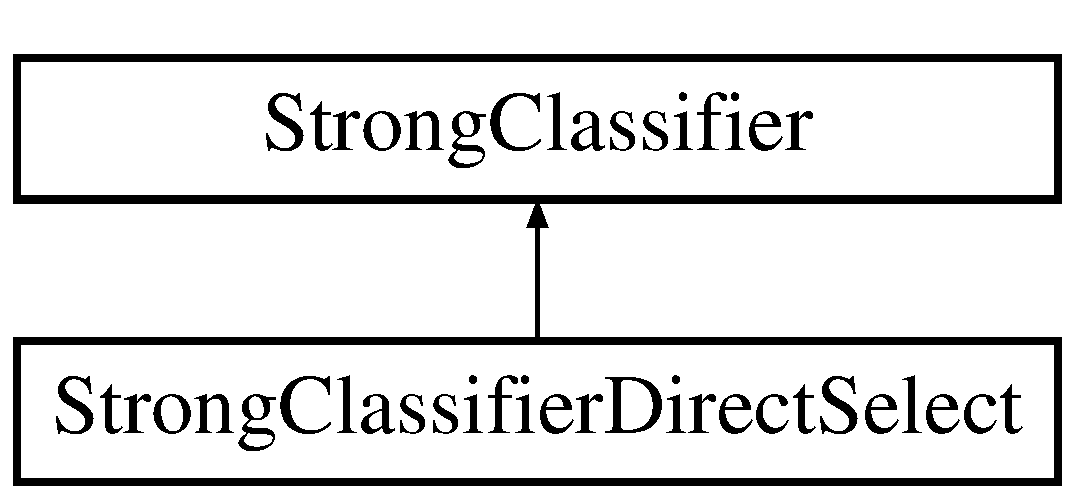
\includegraphics[height=2.000000cm]{classStrongClassifier}
\end{center}
\end{figure}
\subsection*{Public Member Functions}
\begin{DoxyCompactItemize}
\item 
\hypertarget{classStrongClassifier_a98f65a1c2088937ce66f08dc710b178a}{}{\bfseries Strong\+Classifier} (int num\+Selector, int num\+Weak\+Classifier, const \hyperlink{classSize}{Size} \&patch\+Size, bool use\+Feature\+Replace=false, int num\+Backup=0)\label{classStrongClassifier_a98f65a1c2088937ce66f08dc710b178a}

\item 
\hypertarget{classStrongClassifier_a7f2079d46afe7a49cef73a1d8b5fc61d}{}virtual float {\bfseries Evaluate} (const \hyperlink{classIntegralImage}{Integral\+Image} $\ast$int\+Image, const \hyperlink{classRect}{Rect} \&roi) const \label{classStrongClassifier_a7f2079d46afe7a49cef73a1d8b5fc61d}

\item 
\hypertarget{classStrongClassifier_ac6515ad2049961798844049c3ba1e2d6}{}virtual bool {\bfseries Update} (const \hyperlink{classIntegralImage}{Integral\+Image} $\ast$int\+Image, const \hyperlink{classRect}{Rect} \&roi, int target, float importance=1.\+0f)\label{classStrongClassifier_ac6515ad2049961798844049c3ba1e2d6}

\end{DoxyCompactItemize}
\subsection*{Protected Attributes}
\begin{DoxyCompactItemize}
\item 
\hypertarget{classStrongClassifier_ac28de5f3c7dd577833b322f5c2125545}{}int {\bfseries num\+Selector}\label{classStrongClassifier_ac28de5f3c7dd577833b322f5c2125545}

\item 
\hypertarget{classStrongClassifier_adb955a679fec4cc9dc30710381a27e11}{}int {\bfseries total\+Weak\+Classifiers}\label{classStrongClassifier_adb955a679fec4cc9dc30710381a27e11}

\item 
\hypertarget{classStrongClassifier_ad3bcc8911e2308b74f155c09883ac8f2}{}\hyperlink{classClassifierSelector}{Classifier\+Selector} $\ast$$\ast$ {\bfseries selectors}\label{classStrongClassifier_ad3bcc8911e2308b74f155c09883ac8f2}

\item 
\hypertarget{classStrongClassifier_a5f1728b5858ee6db12c796664218278a}{}\hyperlink{classSize}{Size} {\bfseries patch\+Size}\label{classStrongClassifier_a5f1728b5858ee6db12c796664218278a}

\item 
\hypertarget{classStrongClassifier_a57a7599a5b0e2c86e14441f313d0f934}{}float $\ast$ {\bfseries alpha}\label{classStrongClassifier_a57a7599a5b0e2c86e14441f313d0f934}

\item 
\hypertarget{classStrongClassifier_a1115a457d942f20ed7d63325192ff283}{}bool {\bfseries use\+Feature\+Replace}\label{classStrongClassifier_a1115a457d942f20ed7d63325192ff283}

\end{DoxyCompactItemize}


\subsection{Detailed Description}
Use Class\+Selector to build a strong classifier. \begin{DoxyAuthor}{Author}
Zhengrong Wang
\end{DoxyAuthor}
Notice\+: The feature extractor should be prepared (if there are any preprocess procedure), the caller of strong classifier should do that. 

The documentation for this class was generated from the following files\+:\begin{DoxyCompactItemize}
\item 
include/Strong\+Classifier.\+h\item 
src/Strong\+Classifier.\+cpp\end{DoxyCompactItemize}

\hypertarget{classStrongClassifierDirectSelect}{}\section{Strong\+Classifier\+Direct\+Select Class Reference}
\label{classStrongClassifierDirectSelect}\index{Strong\+Classifier\+Direct\+Select@{Strong\+Classifier\+Direct\+Select}}


{\ttfamily \#include $<$Strong\+Classifier\+Direct\+Select.\+h$>$}

Inheritance diagram for Strong\+Classifier\+Direct\+Select\+:\begin{figure}[H]
\begin{center}
\leavevmode
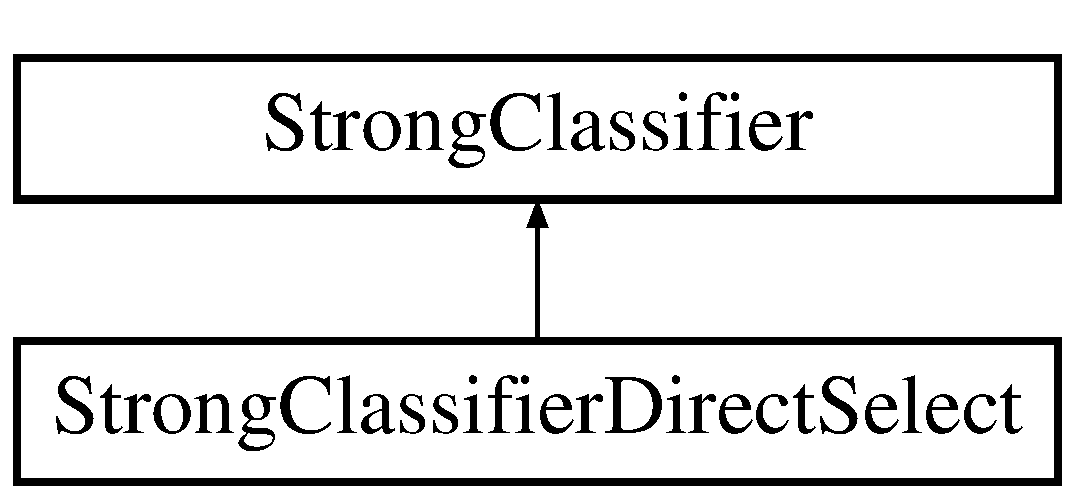
\includegraphics[height=2.000000cm]{classStrongClassifierDirectSelect}
\end{center}
\end{figure}
\subsection*{Public Member Functions}
\begin{DoxyCompactItemize}
\item 
\hypertarget{classStrongClassifierDirectSelect_a9e22d3f25ce43d6f2e3234d502b71df1}{}{\bfseries Strong\+Classifier\+Direct\+Select} (int num\+Selectors, int num\+Weak\+Classifiers, const \hyperlink{classSize}{Size} \&patch\+Size, int num\+Backups=0)\label{classStrongClassifierDirectSelect_a9e22d3f25ce43d6f2e3234d502b71df1}

\item 
virtual void \hyperlink{classStrongClassifierDirectSelect_a423d4e2df75252d92c9e24cb9c37b166}{Initialize} (const \hyperlink{classSize}{Size} \&patch\+Size)
\item 
\hypertarget{classStrongClassifierDirectSelect_a70f5944801a3023fb52e5f69028c76eb}{}virtual bool {\bfseries Update} (const \hyperlink{classIntegralImage}{Integral\+Image} $\ast$int\+Image, const \hyperlink{classRect}{Rect} \&roi, int target, float importance=1.\+0f)\label{classStrongClassifierDirectSelect_a70f5944801a3023fb52e5f69028c76eb}

\end{DoxyCompactItemize}
\subsection*{Additional Inherited Members}


\subsection{Detailed Description}
This strong classifier directly select the best weak classifier and replace the worst one. 

\subsection{Member Function Documentation}
\hypertarget{classStrongClassifierDirectSelect_a423d4e2df75252d92c9e24cb9c37b166}{}\index{Strong\+Classifier\+Direct\+Select@{Strong\+Classifier\+Direct\+Select}!Initialize@{Initialize}}
\index{Initialize@{Initialize}!Strong\+Classifier\+Direct\+Select@{Strong\+Classifier\+Direct\+Select}}
\subsubsection[{Initialize(const Size \&patch\+Size)}]{\setlength{\rightskip}{0pt plus 5cm}void Strong\+Classifier\+Direct\+Select\+::\+Initialize (
\begin{DoxyParamCaption}
\item[{const {\bf Size} \&}]{patch\+Size}
\end{DoxyParamCaption}
)\hspace{0.3cm}{\ttfamily [virtual]}}\label{classStrongClassifierDirectSelect_a423d4e2df75252d92c9e24cb9c37b166}
Initialize a new target for this strong classifier W\+I\+T\+H\+O\+U\+T training. 

Reimplemented from \hyperlink{classStrongClassifier_a4ed37fe7ac50781e4d6ee6271d47731c}{Strong\+Classifier}.



The documentation for this class was generated from the following files\+:\begin{DoxyCompactItemize}
\item 
include/Strong\+Classifier\+Direct\+Select.\+h\item 
src/Strong\+Classifier\+Direct\+Select.\+cpp\end{DoxyCompactItemize}

\hypertarget{classTargetFreeList}{}\section{Target\+Free\+List Class Reference}
\label{classTargetFreeList}\index{Target\+Free\+List@{Target\+Free\+List}}
\subsection*{Public Member Functions}
\begin{DoxyCompactItemize}
\item 
\hypertarget{classTargetFreeList_a28272588d353e55cf201ae0b37598ff8}{}{\bfseries Target\+Free\+List} (int capacity, int num\+Particles, int num\+Selectors, int num\+Weak\+Classifiers, int num\+Backups)\label{classTargetFreeList_a28272588d353e55cf201ae0b37598ff8}

\item 
void \hyperlink{classTargetFreeList_ad9fc512ed531b89b0c1c5d8ff85dd5f7}{Reset\+One\+Target} (int index)
\item 
\hypertarget{classTargetFreeList_a9e78fb14c928075a1eef8bd167f9a3b3}{}int {\bfseries Initialize\+Target} (const \hyperlink{classRect}{Rect} \&target, const \hyperlink{classPoint2D}{Point2\+D} \&init\+Velocity)\label{classTargetFreeList_a9e78fb14c928075a1eef8bd167f9a3b3}

\item 
\hypertarget{classTargetFreeList_a06f32787f7684d164a608ce901fc676b}{}void {\bfseries Propagate} (const \hyperlink{classSize}{Size} \&img\+Size)\label{classTargetFreeList_a06f32787f7684d164a608ce901fc676b}

\end{DoxyCompactItemize}
\subsection*{Public Attributes}
\begin{DoxyCompactItemize}
\item 
\hypertarget{classTargetFreeList_a372b8ad58b14cc943bbba0c5eaf13ab6}{}std\+::vector$<$ \hyperlink{structTargetFreeListNode}{Target\+Free\+List\+Node} $>$ {\bfseries list\+Nodes}\label{classTargetFreeList_a372b8ad58b14cc943bbba0c5eaf13ab6}

\item 
\hypertarget{classTargetFreeList_aae0b9a7f6b9a58348c22b89d3076fad7}{}const int {\bfseries capacity}\label{classTargetFreeList_aae0b9a7f6b9a58348c22b89d3076fad7}

\end{DoxyCompactItemize}


\subsection{Member Function Documentation}
\hypertarget{classTargetFreeList_ad9fc512ed531b89b0c1c5d8ff85dd5f7}{}\index{Target\+Free\+List@{Target\+Free\+List}!Reset\+One\+Target@{Reset\+One\+Target}}
\index{Reset\+One\+Target@{Reset\+One\+Target}!Target\+Free\+List@{Target\+Free\+List}}
\subsubsection[{Reset\+One\+Target(int index)}]{\setlength{\rightskip}{0pt plus 5cm}void Target\+Free\+List\+::\+Reset\+One\+Target (
\begin{DoxyParamCaption}
\item[{int}]{index}
\end{DoxyParamCaption}
)}\label{classTargetFreeList_ad9fc512ed531b89b0c1c5d8ff85dd5f7}
Reset one target. 

The documentation for this class was generated from the following files\+:\begin{DoxyCompactItemize}
\item 
include/Targets\+Free\+List.\+h\item 
src/Tareget\+Free\+List.\+cpp\end{DoxyCompactItemize}

\hypertarget{structTargetFreeListNode}{}\section{Target\+Free\+List\+Node Struct Reference}
\label{structTargetFreeListNode}\index{Target\+Free\+List\+Node@{Target\+Free\+List\+Node}}


{\ttfamily \#include $<$Targets\+Free\+List.\+h$>$}

\subsection*{Public Member Functions}
\begin{DoxyCompactItemize}
\item 
\hypertarget{structTargetFreeListNode_ae75b1f0cf1c490fd85dcf0e20f7c6e2c}{}{\bfseries Target\+Free\+List\+Node} (int num\+Particles, int num\+Selectors, int num\+Weak\+Classifiers, int num\+Backups)\label{structTargetFreeListNode_ae75b1f0cf1c490fd85dcf0e20f7c6e2c}

\end{DoxyCompactItemize}
\subsection*{Public Attributes}
\begin{DoxyCompactItemize}
\item 
\hypertarget{structTargetFreeListNode_a5c4a07cd700b62863f60b45cb6914b1c}{}\hyperlink{classSingleTarget}{Single\+Target} $\ast$ {\bfseries target}\label{structTargetFreeListNode_a5c4a07cd700b62863f60b45cb6914b1c}

\item 
\hypertarget{structTargetFreeListNode_aed70dee64b2cf879cafc5ad0a8d1025f}{}\hyperlink{structTargetFreeListNode}{Target\+Free\+List\+Node} $\ast$ {\bfseries next\+Free}\label{structTargetFreeListNode_aed70dee64b2cf879cafc5ad0a8d1025f}

\item 
\hypertarget{structTargetFreeListNode_a2100999b22ee0afe1ef11e8abc828f66}{}bool {\bfseries is\+Free}\label{structTargetFreeListNode_a2100999b22ee0afe1ef11e8abc828f66}

\end{DoxyCompactItemize}


\subsection{Detailed Description}
This is a container for muiltiple targets.

\begin{DoxyAuthor}{Author}
Zhengrong Wang 
\end{DoxyAuthor}


The documentation for this struct was generated from the following files\+:\begin{DoxyCompactItemize}
\item 
include/Targets\+Free\+List.\+h\item 
src/Tareget\+Free\+List.\+cpp\end{DoxyCompactItemize}

\hypertarget{classTracker}{}\section{Tracker Class Reference}
\label{classTracker}\index{Tracker@{Tracker}}


{\ttfamily \#include $<$Tracker.\+h$>$}

Inheritance diagram for Tracker\+:\begin{figure}[H]
\begin{center}
\leavevmode
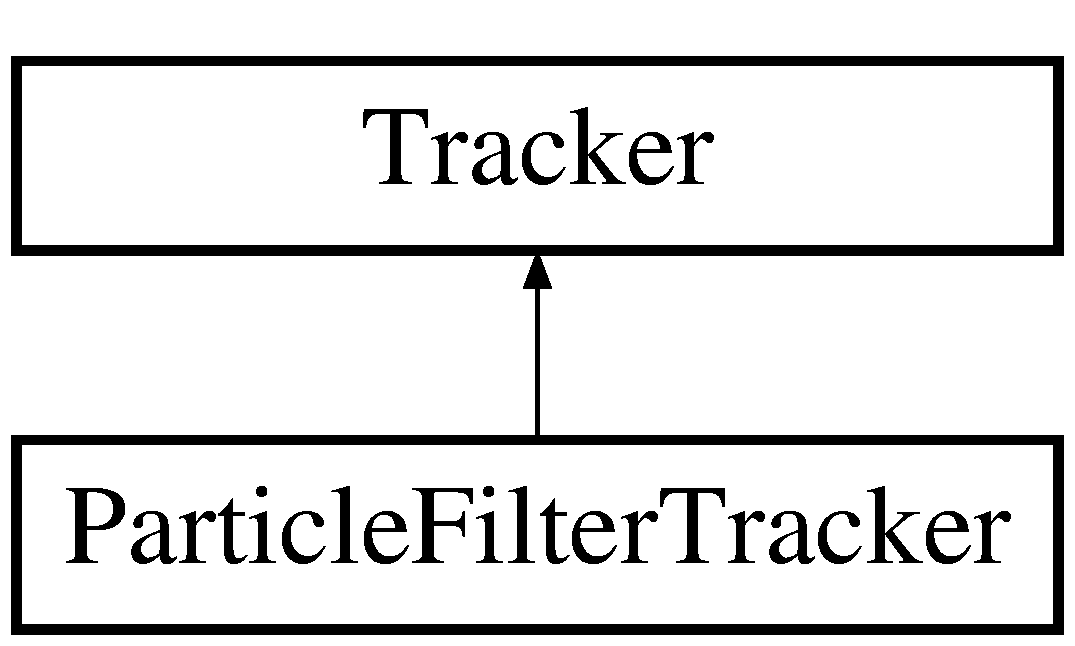
\includegraphics[height=2.000000cm]{classTracker}
\end{center}
\end{figure}
\subsection*{Public Member Functions}
\begin{DoxyCompactItemize}
\item 
\hypertarget{classTracker_a97a7566844820565a36af39560e7b31a}{}virtual void {\bfseries Track} (cv\+::\+Video\+Capture \&in, cv\+::\+Video\+Writer \&out)=0\label{classTracker_a97a7566844820565a36af39560e7b31a}

\end{DoxyCompactItemize}


\subsection{Detailed Description}
\begin{DoxyAuthor}{Author}
Zhengrong Wang. 
\end{DoxyAuthor}


The documentation for this class was generated from the following files\+:\begin{DoxyCompactItemize}
\item 
include/Tracker.\+h\item 
src/Tracker.\+cpp\end{DoxyCompactItemize}

\hypertarget{structTuple}{}\section{Tuple Struct Reference}
\label{structTuple}\index{Tuple@{Tuple}}
\subsection*{Public Attributes}
\begin{DoxyCompactItemize}
\item 
\hypertarget{structTuple_accba76a29fdaf7c297f5b7c1fe0ebd90}{}double {\bfseries attr1}\label{structTuple_accba76a29fdaf7c297f5b7c1fe0ebd90}

\item 
\hypertarget{structTuple_aa1e5aade1f4ed385cc5f9ee9a7ddf80f}{}double {\bfseries attr2}\label{structTuple_aa1e5aade1f4ed385cc5f9ee9a7ddf80f}

\item 
\hypertarget{structTuple_af6d01de2865eb6d35c25e27e36c8616f}{}int {\bfseries num\+\_\+elem}\label{structTuple_af6d01de2865eb6d35c25e27e36c8616f}

\item 
\hypertarget{structTuple_a972e1995023f51c64f972407a6650e1f}{}double $\ast$ {\bfseries data}\label{structTuple_a972e1995023f51c64f972407a6650e1f}

\end{DoxyCompactItemize}


The documentation for this struct was generated from the following file\+:\begin{DoxyCompactItemize}
\item 
include/kmeans.\+h\end{DoxyCompactItemize}

\hypertarget{classUnionFind}{}\section{Union\+Find Class Reference}
\label{classUnionFind}\index{Union\+Find@{Union\+Find}}


{\ttfamily \#include $<$Union\+Find.\+h$>$}

\subsection*{Public Member Functions}
\begin{DoxyCompactItemize}
\item 
\hypertarget{classUnionFind_a686b5bff420abaf11f11e20e692b50e0}{}{\bfseries Union\+Find} (int N)\label{classUnionFind_a686b5bff420abaf11f11e20e692b50e0}

\item 
int \hyperlink{classUnionFind_ab948169c25b587de74e50095120dca88}{Get\+Count} () const 
\item 
int \hyperlink{classUnionFind_a4cd75bd3849d69fbdb186250a3e20ac6}{Get\+Size} (int root)
\item 
int \hyperlink{classUnionFind_a4b831f0ca552a8ba0690c8b6c6012fa6}{Find} (int p) const 
\item 
bool \hyperlink{classUnionFind_a8e5ab36a1cafc1969340cd6102c88c37}{Connected} (int p, int q) const 
\item 
void \hyperlink{classUnionFind_aa999e333a6da859acb9261de757d42f7}{Union} (int p, int q)
\end{DoxyCompactItemize}


\subsection{Detailed Description}
A weighted union find with path compression. \begin{DoxyAuthor}{Author}
Zhengrong Wang 
\end{DoxyAuthor}


\subsection{Member Function Documentation}
\hypertarget{classUnionFind_a8e5ab36a1cafc1969340cd6102c88c37}{}\index{Union\+Find@{Union\+Find}!Connected@{Connected}}
\index{Connected@{Connected}!Union\+Find@{Union\+Find}}
\subsubsection[{Connected(int p, int q) const }]{\setlength{\rightskip}{0pt plus 5cm}bool Union\+Find\+::\+Connected (
\begin{DoxyParamCaption}
\item[{int}]{p, }
\item[{int}]{q}
\end{DoxyParamCaption}
) const\hspace{0.3cm}{\ttfamily [inline]}}\label{classUnionFind_a8e5ab36a1cafc1969340cd6102c88c37}
Are the two sites {\ttfamily p} and {\ttfamily q} in the same component? 
\begin{DoxyParams}{Parameters}
{\em p} & the integer representing one site \\
\hline
{\em q} & the integer representing the other site \\
\hline
\end{DoxyParams}
\begin{DoxyReturn}{Returns}
{\ttfamily true} if the two sites {\ttfamily p} and {\ttfamily q} are in the same component, and {\ttfamily false} otherwise 
\end{DoxyReturn}

\begin{DoxyExceptions}{Exceptions}
{\em java.\+lang.\+Index\+Out\+Of\+Bounds\+Exception} & unless both 0 $<$= p $<$ N and 0 $<$= q $<$ N \\
\hline
\end{DoxyExceptions}
\hypertarget{classUnionFind_a4b831f0ca552a8ba0690c8b6c6012fa6}{}\index{Union\+Find@{Union\+Find}!Find@{Find}}
\index{Find@{Find}!Union\+Find@{Union\+Find}}
\subsubsection[{Find(int p) const }]{\setlength{\rightskip}{0pt plus 5cm}int Union\+Find\+::\+Find (
\begin{DoxyParamCaption}
\item[{int}]{p}
\end{DoxyParamCaption}
) const}\label{classUnionFind_a4b831f0ca552a8ba0690c8b6c6012fa6}
Returns the component identifier for the component containing site {\ttfamily p}. 
\begin{DoxyParams}{Parameters}
{\em p} & the integer representing one site \\
\hline
\end{DoxyParams}
\begin{DoxyReturn}{Returns}
the component identifier for the component containing site {\ttfamily p} 
\end{DoxyReturn}

\begin{DoxyExceptions}{Exceptions}
{\em java.\+lang.\+Index\+Out\+Of\+Bounds\+Exception} & unless 0 $<$= p $<$ N \\
\hline
\end{DoxyExceptions}
\hypertarget{classUnionFind_ab948169c25b587de74e50095120dca88}{}\index{Union\+Find@{Union\+Find}!Get\+Count@{Get\+Count}}
\index{Get\+Count@{Get\+Count}!Union\+Find@{Union\+Find}}
\subsubsection[{Get\+Count() const }]{\setlength{\rightskip}{0pt plus 5cm}int Union\+Find\+::\+Get\+Count (
\begin{DoxyParamCaption}
{}
\end{DoxyParamCaption}
) const\hspace{0.3cm}{\ttfamily [inline]}}\label{classUnionFind_ab948169c25b587de74e50095120dca88}
Returns the number of components. \begin{DoxyReturn}{Returns}
the number of components (between 1 and N) 
\end{DoxyReturn}
\hypertarget{classUnionFind_a4cd75bd3849d69fbdb186250a3e20ac6}{}\index{Union\+Find@{Union\+Find}!Get\+Size@{Get\+Size}}
\index{Get\+Size@{Get\+Size}!Union\+Find@{Union\+Find}}
\subsubsection[{Get\+Size(int root)}]{\setlength{\rightskip}{0pt plus 5cm}int Union\+Find\+::\+Get\+Size (
\begin{DoxyParamCaption}
\item[{int}]{root}
\end{DoxyParamCaption}
)\hspace{0.3cm}{\ttfamily [inline]}}\label{classUnionFind_a4cd75bd3849d69fbdb186250a3e20ac6}
Returns the size of this components. \begin{DoxyReturn}{Returns}
the size of this components (between 1 and N) 
\end{DoxyReturn}
\hypertarget{classUnionFind_aa999e333a6da859acb9261de757d42f7}{}\index{Union\+Find@{Union\+Find}!Union@{Union}}
\index{Union@{Union}!Union\+Find@{Union\+Find}}
\subsubsection[{Union(int p, int q)}]{\setlength{\rightskip}{0pt plus 5cm}void Union\+Find\+::\+Union (
\begin{DoxyParamCaption}
\item[{int}]{p, }
\item[{int}]{q}
\end{DoxyParamCaption}
)}\label{classUnionFind_aa999e333a6da859acb9261de757d42f7}
Merges the component containing site{\ttfamily p} with the component containing site {\ttfamily q}. 
\begin{DoxyParams}{Parameters}
{\em p} & the integer representing one site \\
\hline
{\em q} & the integer representing the other site \\
\hline
\end{DoxyParams}

\begin{DoxyExceptions}{Exceptions}
{\em java.\+lang.\+Index\+Out\+Of\+Bounds\+Exception} & unless both 0 $<$= p $<$ N and 0 $<$= q $<$ N \\
\hline
\end{DoxyExceptions}


The documentation for this class was generated from the following files\+:\begin{DoxyCompactItemize}
\item 
include/Union\+Find.\+h\item 
src/Union\+Find.\+cpp\end{DoxyCompactItemize}

\hypertarget{classVideoDetector}{}\section{Video\+Detector Class Reference}
\label{classVideoDetector}\index{Video\+Detector@{Video\+Detector}}
\subsection*{Public Member Functions}
\begin{DoxyCompactItemize}
\item 
\hypertarget{classVideoDetector_ad8e95ff376d5efa37de2baea11da7757}{}{\bfseries Video\+Detector} (\hyperlink{classImageDetector}{Image\+Detector} $\ast$id, const \hyperlink{structOptions}{Options} \&opt)\label{classVideoDetector_ad8e95ff376d5efa37de2baea11da7757}

\item 
\hypertarget{classVideoDetector_a70bdba6b4f4afc31612ff822927c456d}{}void {\bfseries Detect} (cv\+::\+Video\+Capture \&in, cv\+::\+Video\+Writer \&out, const cv\+::\+Mat \&bkg=default\+Background)\label{classVideoDetector_a70bdba6b4f4afc31612ff822927c456d}

\end{DoxyCompactItemize}
\subsection*{Protected Attributes}
\begin{DoxyCompactItemize}
\item 
\hypertarget{classVideoDetector_aeae5949c4446a47bffcfebc7c1d9cc6e}{}\hyperlink{classImageDetector}{Image\+Detector} $\ast$ {\bfseries img\+Detector}\label{classVideoDetector_aeae5949c4446a47bffcfebc7c1d9cc6e}

\end{DoxyCompactItemize}


The documentation for this class was generated from the following files\+:\begin{DoxyCompactItemize}
\item 
include/Video\+Detector.\+h\item 
src/Video\+Detector.\+cpp\end{DoxyCompactItemize}

\hypertarget{classWeakClassifier}{}\section{Weak\+Classifier Class Reference}
\label{classWeakClassifier}\index{Weak\+Classifier@{Weak\+Classifier}}


{\ttfamily \#include $<$Weak\+Classifier.\+h$>$}

Inheritance diagram for Weak\+Classifier\+:\begin{figure}[H]
\begin{center}
\leavevmode
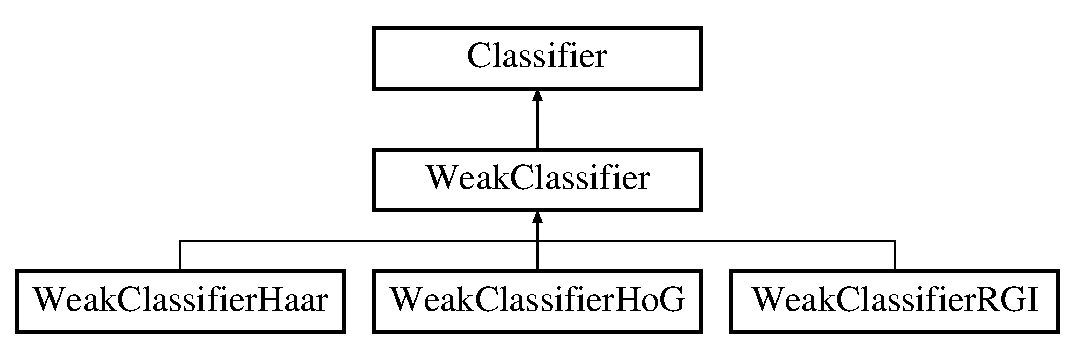
\includegraphics[height=3.000000cm]{classWeakClassifier}
\end{center}
\end{figure}
\subsection*{Public Member Functions}
\begin{DoxyCompactItemize}
\item 
virtual bool \hyperlink{classWeakClassifier_ad4c967e2f0d186a841722f8fea9dbd9c}{Update} (const \hyperlink{classIntegralImage}{Integral\+Image} $\ast$int\+Image, const \hyperlink{classRect}{Rect} \&roi, int target)
\item 
virtual void \hyperlink{classWeakClassifier_a9e62b318d87b30965646bdc94662c01d}{Initialize} (const \hyperlink{classSize}{Size} \&patch\+Size)
\item 
virtual float \hyperlink{classWeakClassifier_a083dddaa52fe399386f07a20f231ec49}{Evaluate} (const \hyperlink{classIntegralImage}{Integral\+Image} $\ast$int\+Image, const \hyperlink{classRect}{Rect} \&roi)
\end{DoxyCompactItemize}


\subsection{Detailed Description}
This is an interface. \begin{DoxyAuthor}{Author}
Zhengrong Wang. 
\end{DoxyAuthor}


\subsection{Member Function Documentation}
\hypertarget{classWeakClassifier_a083dddaa52fe399386f07a20f231ec49}{}\index{Weak\+Classifier@{Weak\+Classifier}!Evaluate@{Evaluate}}
\index{Evaluate@{Evaluate}!Weak\+Classifier@{Weak\+Classifier}}
\subsubsection[{Evaluate(const Integral\+Image $\ast$int\+Image, const Rect \&roi)}]{\setlength{\rightskip}{0pt plus 5cm}float Weak\+Classifier\+::\+Evaluate (
\begin{DoxyParamCaption}
\item[{const {\bf Integral\+Image} $\ast$}]{int\+Image, }
\item[{const {\bf Rect} \&}]{roi}
\end{DoxyParamCaption}
)\hspace{0.3cm}{\ttfamily [virtual]}}\label{classWeakClassifier_a083dddaa52fe399386f07a20f231ec49}
\begin{DoxyReturn}{Returns}
\mbox{[}0.\+0, 1.\+0\mbox{]} 
\end{DoxyReturn}


Reimplemented in \hyperlink{classWeakClassifierHaar_a5880dbf4a75a29e61e32903faef1dae6}{Weak\+Classifier\+Haar}, and \hyperlink{classWeakClassifierRGI_aaff18f2962e93ad64eb7b4c6e127b91c}{Weak\+Classifier\+R\+G\+I}.

\hypertarget{classWeakClassifier_a9e62b318d87b30965646bdc94662c01d}{}\index{Weak\+Classifier@{Weak\+Classifier}!Initialize@{Initialize}}
\index{Initialize@{Initialize}!Weak\+Classifier@{Weak\+Classifier}}
\subsubsection[{Initialize(const Size \&patch\+Size)}]{\setlength{\rightskip}{0pt plus 5cm}void Weak\+Classifier\+::\+Initialize (
\begin{DoxyParamCaption}
\item[{const {\bf Size} \&}]{patch\+Size}
\end{DoxyParamCaption}
)\hspace{0.3cm}{\ttfamily [virtual]}}\label{classWeakClassifier_a9e62b318d87b30965646bdc94662c01d}
Initialize the weak classifier. 

Reimplemented in \hyperlink{classWeakClassifierHaar_ac5e1a9ff691bd0dcf9174af88cc9dc1f}{Weak\+Classifier\+Haar}, and \hyperlink{classWeakClassifierRGI_af3d14f1749fa8543ac6f3e52af2cf607}{Weak\+Classifier\+R\+G\+I}.

\hypertarget{classWeakClassifier_ad4c967e2f0d186a841722f8fea9dbd9c}{}\index{Weak\+Classifier@{Weak\+Classifier}!Update@{Update}}
\index{Update@{Update}!Weak\+Classifier@{Weak\+Classifier}}
\subsubsection[{Update(const Integral\+Image $\ast$int\+Image, const Rect \&roi, int target)}]{\setlength{\rightskip}{0pt plus 5cm}bool Weak\+Classifier\+::\+Update (
\begin{DoxyParamCaption}
\item[{const {\bf Integral\+Image} $\ast$}]{int\+Image, }
\item[{const {\bf Rect} \&}]{roi, }
\item[{int}]{target}
\end{DoxyParamCaption}
)\hspace{0.3cm}{\ttfamily [virtual]}}\label{classWeakClassifier_ad4c967e2f0d186a841722f8fea9dbd9c}
Update this weak classifer. Return true if after update, this weak classifer still can not classify this sample correctly. 

Reimplemented in \hyperlink{classWeakClassifierHaar_aa8dc6734dc435c246d9605aceea2c9a7}{Weak\+Classifier\+Haar}, and \hyperlink{classWeakClassifierRGI_ab4719f5dcf7acf6e79beb4d246addaa5}{Weak\+Classifier\+R\+G\+I}.



The documentation for this class was generated from the following files\+:\begin{DoxyCompactItemize}
\item 
include/Weak\+Classifier.\+h\item 
src/Weak\+Classifier.\+cpp\end{DoxyCompactItemize}

\hypertarget{classWeakClassifierHaar}{}\section{Weak\+Classifier\+Haar Class Reference}
\label{classWeakClassifierHaar}\index{Weak\+Classifier\+Haar@{Weak\+Classifier\+Haar}}


{\ttfamily \#include $<$Weak\+Classifier\+Haar.\+h$>$}

Inheritance diagram for Weak\+Classifier\+Haar\+:\begin{figure}[H]
\begin{center}
\leavevmode
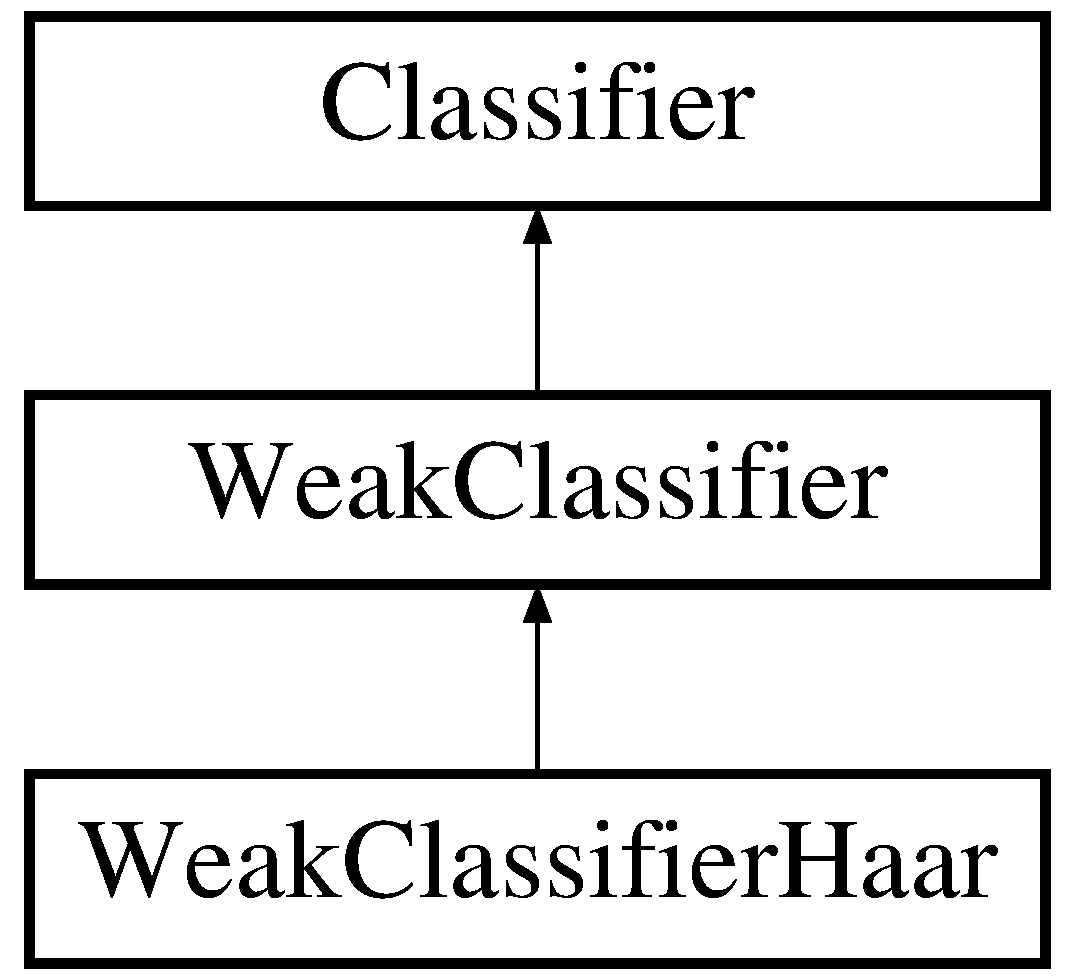
\includegraphics[height=3.000000cm]{classWeakClassifierHaar}
\end{center}
\end{figure}
\subsection*{Public Member Functions}
\begin{DoxyCompactItemize}
\item 
\hypertarget{classWeakClassifierHaar_a5897c0e554cb8e3dd0cb001bb76a3c93}{}{\bfseries Weak\+Classifier\+Haar} (const \hyperlink{classSize}{Size} \&patch\+Size)\label{classWeakClassifierHaar_a5897c0e554cb8e3dd0cb001bb76a3c93}

\item 
bool \hyperlink{classWeakClassifierHaar_aa8dc6734dc435c246d9605aceea2c9a7}{Update} (const \hyperlink{classIntegralImage}{Integral\+Image} $\ast$int\+Image, const \hyperlink{classRect}{Rect} \&roi, int target)
\item 
\hypertarget{classWeakClassifierHaar_a2b7ad8b6691f6739ebe75c5301fa252b}{}int {\bfseries Classify} (const \hyperlink{classIntegralImage}{Integral\+Image} $\ast$int\+Image, const \hyperlink{classRect}{Rect} \&roi, float scale=1.\+0f)\label{classWeakClassifierHaar_a2b7ad8b6691f6739ebe75c5301fa252b}

\item 
float \hyperlink{classWeakClassifierHaar_a5880dbf4a75a29e61e32903faef1dae6}{Evaluate} (const \hyperlink{classIntegralImage}{Integral\+Image} $\ast$int\+Image, const \hyperlink{classRect}{Rect} \&roi)
\item 
\hypertarget{classWeakClassifierHaar_ac577e6b2c75eb48bc93068966c522f3f}{}void {\bfseries Reset\+Pos\+Dist} ()\label{classWeakClassifierHaar_ac577e6b2c75eb48bc93068966c522f3f}

\end{DoxyCompactItemize}


\subsection{Detailed Description}
Using Haar \hyperlink{classFeature}{Feature} to construct a weak classifier. Also estimate the positive and negative cluster with Kalman filter. \begin{DoxyAuthor}{Author}
Zhengrong Wang. 
\end{DoxyAuthor}


\subsection{Member Function Documentation}
\hypertarget{classWeakClassifierHaar_a5880dbf4a75a29e61e32903faef1dae6}{}\index{Weak\+Classifier\+Haar@{Weak\+Classifier\+Haar}!Evaluate@{Evaluate}}
\index{Evaluate@{Evaluate}!Weak\+Classifier\+Haar@{Weak\+Classifier\+Haar}}
\subsubsection[{Evaluate(const Integral\+Image $\ast$int\+Image, const Rect \&roi)}]{\setlength{\rightskip}{0pt plus 5cm}float Weak\+Classifier\+Haar\+::\+Evaluate (
\begin{DoxyParamCaption}
\item[{const {\bf Integral\+Image} $\ast$}]{int\+Image, }
\item[{const {\bf Rect} \&}]{roi}
\end{DoxyParamCaption}
)\hspace{0.3cm}{\ttfamily [virtual]}}\label{classWeakClassifierHaar_a5880dbf4a75a29e61e32903faef1dae6}
\begin{DoxyReturn}{Returns}
\mbox{[}0.\+0, 1.\+0\mbox{]} 
\end{DoxyReturn}


Reimplemented from \hyperlink{classWeakClassifier_a083dddaa52fe399386f07a20f231ec49}{Weak\+Classifier}.

\hypertarget{classWeakClassifierHaar_aa8dc6734dc435c246d9605aceea2c9a7}{}\index{Weak\+Classifier\+Haar@{Weak\+Classifier\+Haar}!Update@{Update}}
\index{Update@{Update}!Weak\+Classifier\+Haar@{Weak\+Classifier\+Haar}}
\subsubsection[{Update(const Integral\+Image $\ast$int\+Image, const Rect \&roi, int target)}]{\setlength{\rightskip}{0pt plus 5cm}bool Weak\+Classifier\+Haar\+::\+Update (
\begin{DoxyParamCaption}
\item[{const {\bf Integral\+Image} $\ast$}]{int\+Image, }
\item[{const {\bf Rect} \&}]{roi, }
\item[{int}]{target}
\end{DoxyParamCaption}
)\hspace{0.3cm}{\ttfamily [virtual]}}\label{classWeakClassifierHaar_aa8dc6734dc435c246d9605aceea2c9a7}
Update this weak classifer. Return true if after update, this weak classifer still can not classify this sample correctly. 

Reimplemented from \hyperlink{classWeakClassifier_ad4c967e2f0d186a841722f8fea9dbd9c}{Weak\+Classifier}.



The documentation for this class was generated from the following files\+:\begin{DoxyCompactItemize}
\item 
include/Weak\+Classifier\+Haar.\+h\item 
src/Weak\+Classifier\+Haar.\+cpp\end{DoxyCompactItemize}

\hypertarget{classWeakClassifierHoG}{}\section{Weak\+Classifier\+Ho\+G Class Reference}
\label{classWeakClassifierHoG}\index{Weak\+Classifier\+Ho\+G@{Weak\+Classifier\+Ho\+G}}


{\ttfamily \#include $<$Weak\+Classifier\+Ho\+G.\+h$>$}

Inheritance diagram for Weak\+Classifier\+Ho\+G\+:\begin{figure}[H]
\begin{center}
\leavevmode
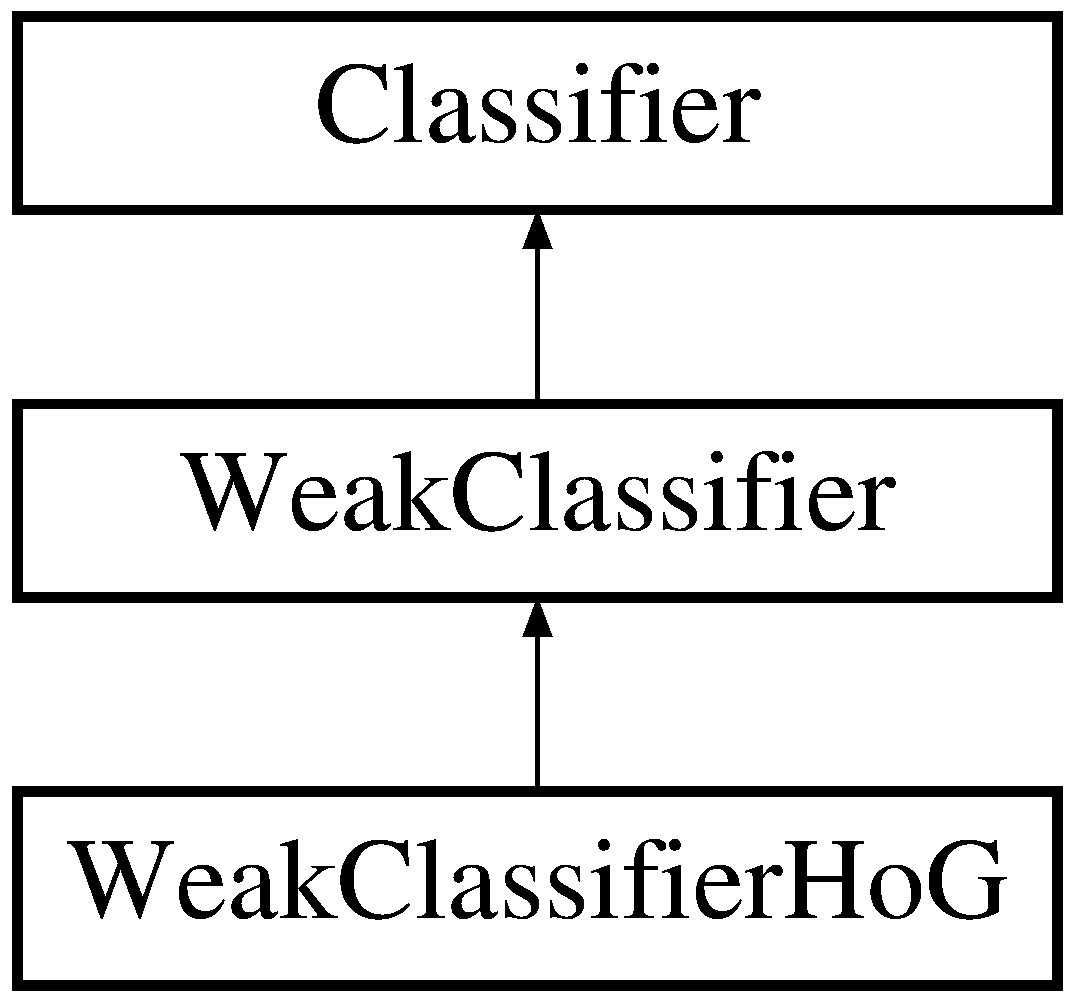
\includegraphics[height=3.000000cm]{classWeakClassifierHoG}
\end{center}
\end{figure}
\subsection*{Public Member Functions}
\begin{DoxyCompactItemize}
\item 
\hyperlink{classWeakClassifierHoG_a1355cfb6af523b56b52ff27b88eb066c}{Weak\+Classifier\+Ho\+G} (const \hyperlink{classFeature}{Feature} \&reference, float min, float max, int offset\+W, int offset\+H, int w, int h, float $\ast$histogram)
\item 
float \hyperlink{classWeakClassifierHoG_aef5482b7842e91410c9186c242ee0d6b}{Evaluate} (const \hyperlink{classIntegralImage}{Integral\+Image} $\ast$int\+Image, const \hyperlink{classRect}{Rect} \&roi, float scale=1.\+0f)
\item 
float \hyperlink{classWeakClassifierHoG_a5b0ecb768ced4b91d1bb0ddf214f4ac6}{Evaluate\+Thre} (const \hyperlink{classIntegralImage}{Integral\+Image} $\ast$int\+Image, const \hyperlink{classRect}{Rect} \&roi, float scale=1.\+0f)
\end{DoxyCompactItemize}


\subsection{Detailed Description}
Given a roi in an image, finds the Ho\+G in some subregion and project it to get some value. \begin{DoxyAuthor}{Author}
\+: Zhengrong Wang. 
\end{DoxyAuthor}


\subsection{Constructor \& Destructor Documentation}
\hypertarget{classWeakClassifierHoG_a1355cfb6af523b56b52ff27b88eb066c}{}\index{Weak\+Classifier\+Ho\+G@{Weak\+Classifier\+Ho\+G}!Weak\+Classifier\+Ho\+G@{Weak\+Classifier\+Ho\+G}}
\index{Weak\+Classifier\+Ho\+G@{Weak\+Classifier\+Ho\+G}!Weak\+Classifier\+Ho\+G@{Weak\+Classifier\+Ho\+G}}
\subsubsection[{Weak\+Classifier\+Ho\+G(const Feature \&reference, float min, float max, int offset\+W, int offset\+H, int w, int h, float $\ast$histogram)}]{\setlength{\rightskip}{0pt plus 5cm}Weak\+Classifier\+Ho\+G\+::\+Weak\+Classifier\+Ho\+G (
\begin{DoxyParamCaption}
\item[{const {\bf Feature} \&}]{reference, }
\item[{float}]{min, }
\item[{float}]{max, }
\item[{int}]{offset\+W, }
\item[{int}]{offset\+H, }
\item[{int}]{w, }
\item[{int}]{h, }
\item[{float $\ast$}]{histogram}
\end{DoxyParamCaption}
)}\label{classWeakClassifierHoG_a1355cfb6af523b56b52ff27b88eb066c}
Construct a weak classifier. 
\begin{DoxyParams}{Parameters}
{\em reference} & the reference for this weak classifier. \\
\hline
{\em min,max} & used to find the histogram.  histogram\+: histogram. \\
\hline
{\em others} & for the \hyperlink{classHoGFeature}{Ho\+G\+Feature}. \\
\hline
\end{DoxyParams}


\subsection{Member Function Documentation}
\hypertarget{classWeakClassifierHoG_aef5482b7842e91410c9186c242ee0d6b}{}\index{Weak\+Classifier\+Ho\+G@{Weak\+Classifier\+Ho\+G}!Evaluate@{Evaluate}}
\index{Evaluate@{Evaluate}!Weak\+Classifier\+Ho\+G@{Weak\+Classifier\+Ho\+G}}
\subsubsection[{Evaluate(const Integral\+Image $\ast$int\+Image, const Rect \&roi, float scale=1.\+0f)}]{\setlength{\rightskip}{0pt plus 5cm}float Weak\+Classifier\+Ho\+G\+::\+Evaluate (
\begin{DoxyParamCaption}
\item[{const {\bf Integral\+Image} $\ast$}]{int\+Image, }
\item[{const {\bf Rect} \&}]{roi, }
\item[{float}]{scale = {\ttfamily 1.0f}}
\end{DoxyParamCaption}
)\hspace{0.3cm}{\ttfamily [virtual]}}\label{classWeakClassifierHoG_aef5482b7842e91410c9186c242ee0d6b}
Return the dot product between the reference and result. 

Reimplemented from \hyperlink{classClassifier}{Classifier}.

\hypertarget{classWeakClassifierHoG_a5b0ecb768ced4b91d1bb0ddf214f4ac6}{}\index{Weak\+Classifier\+Ho\+G@{Weak\+Classifier\+Ho\+G}!Evaluate\+Thre@{Evaluate\+Thre}}
\index{Evaluate\+Thre@{Evaluate\+Thre}!Weak\+Classifier\+Ho\+G@{Weak\+Classifier\+Ho\+G}}
\subsubsection[{Evaluate\+Thre(const Integral\+Image $\ast$int\+Image, const Rect \&roi, float scale=1.\+0f)}]{\setlength{\rightskip}{0pt plus 5cm}float Weak\+Classifier\+Ho\+G\+::\+Evaluate\+Thre (
\begin{DoxyParamCaption}
\item[{const {\bf Integral\+Image} $\ast$}]{int\+Image, }
\item[{const {\bf Rect} \&}]{roi, }
\item[{float}]{scale = {\ttfamily 1.0f}}
\end{DoxyParamCaption}
)}\label{classWeakClassifierHoG_a5b0ecb768ced4b91d1bb0ddf214f4ac6}
Return the increament in threshold. Used in Ada\+Boosting classifier. 

The documentation for this class was generated from the following files\+:\begin{DoxyCompactItemize}
\item 
include/Weak\+Classifier\+Ho\+G.\+h\item 
src/Weak\+Classifier\+Ho\+G.\+cpp\end{DoxyCompactItemize}

\hypertarget{classWeakClassifierRGI}{}\section{Weak\+Classifier\+R\+G\+I Class Reference}
\label{classWeakClassifierRGI}\index{Weak\+Classifier\+R\+G\+I@{Weak\+Classifier\+R\+G\+I}}


{\ttfamily \#include $<$Weak\+Classifier\+R\+G\+I.\+h$>$}

Inheritance diagram for Weak\+Classifier\+R\+G\+I\+:\begin{figure}[H]
\begin{center}
\leavevmode
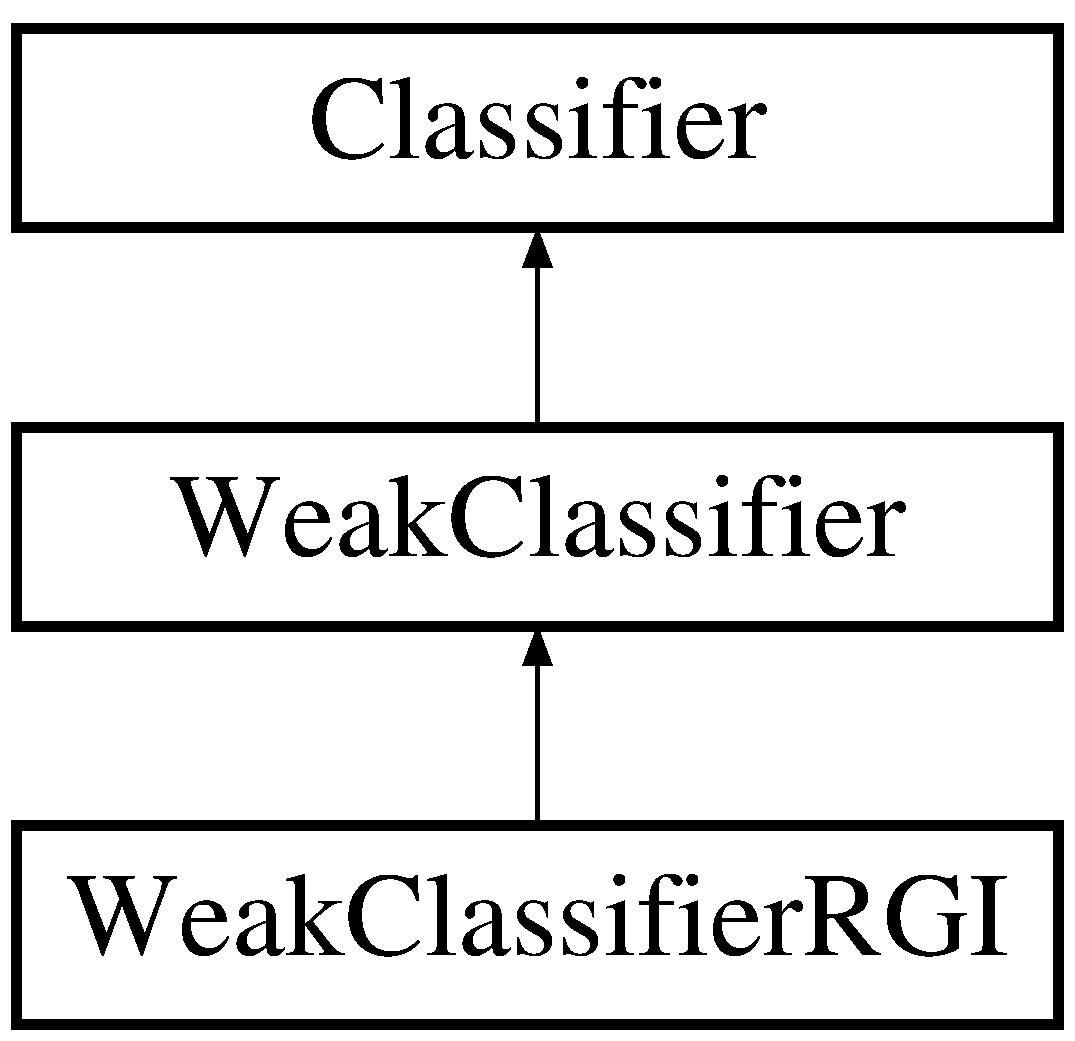
\includegraphics[height=3.000000cm]{classWeakClassifierRGI}
\end{center}
\end{figure}
\subsection*{Public Member Functions}
\begin{DoxyCompactItemize}
\item 
\hypertarget{classWeakClassifierRGI_abbd6a27d77c3f38bcf2dce39d7571cf7}{}{\bfseries Weak\+Classifier\+R\+G\+I} (const \hyperlink{classSize}{Size} \&patch\+Size)\label{classWeakClassifierRGI_abbd6a27d77c3f38bcf2dce39d7571cf7}

\item 
virtual bool \hyperlink{classWeakClassifierRGI_ab4719f5dcf7acf6e79beb4d246addaa5}{Update} (const \hyperlink{classIntegralImage}{Integral\+Image} $\ast$int\+Image, const \hyperlink{classRect}{Rect} \&roi, int target)
\item 
\hypertarget{classWeakClassifierRGI_a026ab7a9f1c19ced68746121aacd6374}{}virtual int {\bfseries Classify} (const \hyperlink{classIntegralImage}{Integral\+Image} $\ast$int\+Image, const \hyperlink{classRect}{Rect} \&roi, float scale=1.\+0f)\label{classWeakClassifierRGI_a026ab7a9f1c19ced68746121aacd6374}

\item 
virtual float \hyperlink{classWeakClassifierRGI_aaff18f2962e93ad64eb7b4c6e127b91c}{Evaluate} (const \hyperlink{classIntegralImage}{Integral\+Image} $\ast$int\+Image, const \hyperlink{classRect}{Rect} \&roi)
\item 
virtual void \hyperlink{classWeakClassifierRGI_af3d14f1749fa8543ac6f3e52af2cf607}{Initialize} (const \hyperlink{classSize}{Size} \&patch\+Size)
\item 
\hypertarget{classWeakClassifierRGI_aa48904ae41002320da3e5563aaf1ca60}{}void {\bfseries Reset\+Pos\+Dist} ()\label{classWeakClassifierRGI_aa48904ae41002320da3e5563aaf1ca60}

\end{DoxyCompactItemize}


\subsection{Detailed Description}
Using R\+G\+I feature to construct a weak classifier. \begin{DoxyAuthor}{Author}
Zhengrong Wang 
\end{DoxyAuthor}


\subsection{Member Function Documentation}
\hypertarget{classWeakClassifierRGI_aaff18f2962e93ad64eb7b4c6e127b91c}{}\index{Weak\+Classifier\+R\+G\+I@{Weak\+Classifier\+R\+G\+I}!Evaluate@{Evaluate}}
\index{Evaluate@{Evaluate}!Weak\+Classifier\+R\+G\+I@{Weak\+Classifier\+R\+G\+I}}
\subsubsection[{Evaluate(const Integral\+Image $\ast$int\+Image, const Rect \&roi)}]{\setlength{\rightskip}{0pt plus 5cm}float Weak\+Classifier\+R\+G\+I\+::\+Evaluate (
\begin{DoxyParamCaption}
\item[{const {\bf Integral\+Image} $\ast$}]{int\+Image, }
\item[{const {\bf Rect} \&}]{roi}
\end{DoxyParamCaption}
)\hspace{0.3cm}{\ttfamily [virtual]}}\label{classWeakClassifierRGI_aaff18f2962e93ad64eb7b4c6e127b91c}
\begin{DoxyReturn}{Returns}
\mbox{[}0.\+0, 1.\+0\mbox{]} 
\end{DoxyReturn}


Reimplemented from \hyperlink{classWeakClassifier_a083dddaa52fe399386f07a20f231ec49}{Weak\+Classifier}.

\hypertarget{classWeakClassifierRGI_af3d14f1749fa8543ac6f3e52af2cf607}{}\index{Weak\+Classifier\+R\+G\+I@{Weak\+Classifier\+R\+G\+I}!Initialize@{Initialize}}
\index{Initialize@{Initialize}!Weak\+Classifier\+R\+G\+I@{Weak\+Classifier\+R\+G\+I}}
\subsubsection[{Initialize(const Size \&patch\+Size)}]{\setlength{\rightskip}{0pt plus 5cm}void Weak\+Classifier\+R\+G\+I\+::\+Initialize (
\begin{DoxyParamCaption}
\item[{const {\bf Size} \&}]{patch\+Size}
\end{DoxyParamCaption}
)\hspace{0.3cm}{\ttfamily [virtual]}}\label{classWeakClassifierRGI_af3d14f1749fa8543ac6f3e52af2cf607}
Initialize the weak classifier. 

Reimplemented from \hyperlink{classWeakClassifier_a9e62b318d87b30965646bdc94662c01d}{Weak\+Classifier}.

\hypertarget{classWeakClassifierRGI_ab4719f5dcf7acf6e79beb4d246addaa5}{}\index{Weak\+Classifier\+R\+G\+I@{Weak\+Classifier\+R\+G\+I}!Update@{Update}}
\index{Update@{Update}!Weak\+Classifier\+R\+G\+I@{Weak\+Classifier\+R\+G\+I}}
\subsubsection[{Update(const Integral\+Image $\ast$int\+Image, const Rect \&roi, int target)}]{\setlength{\rightskip}{0pt plus 5cm}bool Weak\+Classifier\+R\+G\+I\+::\+Update (
\begin{DoxyParamCaption}
\item[{const {\bf Integral\+Image} $\ast$}]{int\+Image, }
\item[{const {\bf Rect} \&}]{roi, }
\item[{int}]{target}
\end{DoxyParamCaption}
)\hspace{0.3cm}{\ttfamily [virtual]}}\label{classWeakClassifierRGI_ab4719f5dcf7acf6e79beb4d246addaa5}
Update this weak classifer. Return true if after update, this weak classifer still can not classify this sample correctly. 

Reimplemented from \hyperlink{classWeakClassifier_ad4c967e2f0d186a841722f8fea9dbd9c}{Weak\+Classifier}.



The documentation for this class was generated from the following files\+:\begin{DoxyCompactItemize}
\item 
include/Weak\+Classifier\+R\+G\+I.\+h\item 
src/Weak\+Classifier\+R\+G\+I.\+cpp\end{DoxyCompactItemize}

%--- End generated contents ---

% Index
\backmatter
\newpage
\phantomsection
\clearemptydoublepage
\addcontentsline{toc}{chapter}{Index}
\printindex

\end{document}
